\documentclass[12pt]{gatechthesis}

\renewcommand{\baselinestretch}{1.3}

%external commands
\newcommand{\todo}[1]{\noindent{\color{red}{\bf \fbox{TODO}}{\it#1}}}
\newcommand\epulsar{\textbf{ePulsar }}
\newcommand\oneedge{\textbf{OneEdge}}
\newcommand\onefog{\oneedge}
\newcommand{\UDC}{$\mu$DC\xspace}



%packages
\usepackage{comment}

\usepackage{textcomp}
\usepackage{subcaption}
\usepackage{listings}
\usepackage{xcolor}

\colorlet{punct}{red!60!black}
\definecolor{background}{HTML}{EEEEEE}
\definecolor{delim}{RGB}{20,105,176}
\colorlet{numb}{magenta!60!black}
\lstdefinelanguage{json}{
    basicstyle=\normalfont\ttfamily,
    %numbers=left,
    numberstyle=\scriptsize,
    stepnumber=1,
    numbersep=8pt,
    showstringspaces=false,
    breaklines=true,
    frame=lines,
    backgroundcolor=\color{background},
    literate=
     *{0}{{{\color{numb}0}}}{1}
      {1}{{{\color{numb}1}}}{1}
      {2}{{{\color{numb}2}}}{1}
      {3}{{{\color{numb}3}}}{1}
      {4}{{{\color{numb}4}}}{1}
      {5}{{{\color{numb}5}}}{1}
      {6}{{{\color{numb}6}}}{1}
      {7}{{{\color{numb}7}}}{1}
      {8}{{{\color{numb}8}}}{1}
      {9}{{{\color{numb}9}}}{1}
      {:}{{{\color{punct}{:}}}}{1}
      {,}{{{\color{punct}{,}}}}{1}
      {\{}{{{\color{delim}{\{}}}}{1}
      {\}}{{{\color{delim}{\}}}}}{1}
      {[}{{{\color{delim}{[}}}}{1}
      {]}{{{\color{delim}{]}}}}{1},
}

\usepackage{amsmath}
\usepackage{algorithm}
\usepackage[normalem]{ulem}
\usepackage{verbatim}
\usepackage[noend]{algpseudocode}
\usepackage{minted}
\usepackage[capitalise]{cleveref}
\usepackage{hyperref}
% preamble

\title{Mechanisms for compute and data orchestration for geo-distributed situation-awareness applications on edge infrastructure}
\author{Harshit Gupta}
\approvaldate{December 6, 2021}
\school{School of Computer Science}
\department{College of Computing}
\bibliography{references}

% document body
\begin{document}

\makeTitlePage{December}{2021}
%
% In \begin{approvalPage}{N}, the parameter N is the number of members in the committee. If this is less than 4, the layout of the page is single-column rather than two-column, so change the value accordingly.

\begin{approvalPage}{5}

% Add people in the following format:
% \committeeMember{Member Name}{Member Department/Position}{Member Affiliation}

\committeeMember{Professor Umakishore Ramachandran, Advisor}{School of Computer Science}{Georgia Institute of
Technology}
\committeeMember{Professor Ada Gavrilovska}{School of Computer Science}{Georgia Institute of Technology}
\committeeMember{Professor Alexandros Daglis}{School of Computer Science}{Georgia Institute of Technology}
\committeeMember{Professor Ahmed Saeed}{School of Computer Science}{Georgia Institute of Technology}
\committeeMember{Dr. Abhigyan Sharma}{Meta}
\\ % <- add space for alignment, if necessary

\end{approvalPage}
%\makeEpigraph{I'm not super. Any talents I have, I worked for -- it seems a long time since I thought of myself as a hero.}{Oliver Queen}
%\makeDedication{For my wife Laura}

\begin{frontmatter}
    %
\begin{acknowledgments}


\end{acknowledgments}

    \makeTOC
    \makeListOfTables
    \makeListOfFigures
    \newcommand{\newdefinedabbreviation}[3]{
    \newglossaryentry{#1}
    {
      type=\acronymtype, 
      name={#2},
      description={#3},
      first={#3 (#2)},
      plural={{#2}s},
      descriptionplural={{#3}s},
      firstplural={{#3}s ({#2}s)}
    }
}

\newcommand{\newdefinedabbreviationwithplural}[4]{
    \newglossaryentry{#1}
    {
      type=\acronymtype, 
      name={#2},
      description={#3},
      first={#3 (#2)},
      plural={{#2}s},
      descriptionplural={#4},
      firstplural={#4 ({#2}s)}
    }
}

\newdefinedabbreviation{dc}{DC}{datacenter}
\newdefinedabbreviation{dfg}{DFG}{dataflow graph}
\newdefinedabbreviation{slo}{SLO}{service-level objective}
\newdefinedabbreviation{sla}{SLA}{service-level agreement}
\newdefinedabbreviation{iot}{IoT}{internet of things}
\newdefinedabbreviation{wan}{WAN}{wide-area network}
\newdefinedabbreviation{qos}{QoS}{quality-of-service}
\newdefinedabbreviation{vm}{VM}{Virtual Machine}
\newdefinedabbreviation{hud}{HUD}{Heads-up Display}
\newdefinedabbreviation{uav}{UAV}{Unmanned Aerial Vehicle}
\newdefinedabbreviation{ptz}{PTZ}{Pan-Tilt-Zoom}
\newdefinedabbreviation{lidar}{LiDAR}{Light Detection and Ranging}
\newdefinedabbreviation{cdf}{CDF}{Cumulative Distribution Function}
\newdefinedabbreviation{rnis}{RNIS}{Radio Network Information Service}
\newdefinedabbreviation{rtt}{RTT}{Round Trip Time}
\newdefinedabbreviationwithplural{aoi}{AoI}{Area of Interest}{Areas of Interest}
%\newdefinedabbreviation{aoi}{AoI}{Area of Interest}
\makeListOfAcronyms
%\newdefinedabbreviation{udc}{{\textmu}DC}{micro-datacenter}
%\newdefinedabbreviation{ar}{AR}{augmented reality}
%\newdefinedabbreviation{e2e}{E2E}{end-to-end}

%\newdefinedabbreviation{api}{API}{application programming interface}
%\newdefinedabbreviation{rrp}{RRP}{resource requirement profile}
%\newdefinedabbreviation{2pc}{2PC}{two-phase commit}
%\newdefinedabbreviation{mcf}{MCF}{mean conflict fraction}
%\newdefinedabbreviation{rtt}{RTT}{round-trip time}

%\printglossaries


    \begin{summary}
Situation-awareness applications require low-latency response and impose significant network bandwidth requirements, and hence benefit from geo-distributed Edge infrastructure. These applications rely on several platform services, such as Kubernetes, Apache Cassandra and Pulsar, for managing their compute and data components. These platform services are responsible for scheduling compute components and placing data across the geo-distributed Edge infrastructure, which has strong implications on the applications’ response time. Hosting situation-awareness applications on Edge infrastructure poses novel requirements on the platform services. Firstly, the processing logic of these applications is closely tied to the physical environment that it is interacting with. Hence, the access pattern to compute and data exhibits strong spatial affinity. Secondly, the network topology of Edge infrastructure is heterogeneous, wherein communication latency forms a significant portion of the end-to-end response time of the application. Finally, clients of situation-awareness applications are inherently mobile, which necessitates continuous adaptation of compute and data placement decisions to ensure latency requirements are satisfied while adhering to spatial affinity requirements.

The control planes of off-the-shelf platform services do not have the necessary primitives to incorporate spatial affinity and network topology awareness into the compute and data orchestration policies. They also do not perform fine-grained end-to-end monitoring of application response times to detect and adapt to performance degradations due to client mobility. This dissertation presents three mechanisms that inform the compute/data placement policies for platform services, so that application performance requirements can be met.
\begin{itemize}
\item Distributed spatial context management for system entities - including clients and data/compute components to ensure spatial affinity constraints are satisfied.
\item Topology awareness through scalable network proximity estimation among clients and Edge sites.
\item Distributed platform for fine-grained monitoring and aggregation of per-application metrics that provides end-to-end insights into application performance.
\end{itemize}
The thesis of our work is that such mechanisms are essential for meeting the quality of service guarantees for situation-awareness applications on geo-distributed infrastructures. We demonstrate by construction the efficacy and scalability of the proposed mechanisms for building dynamic compute and data orchestration policies by incorporating them in the control planes of three different platform services. Specifically, we incorporate these mechanisms into a topic-based publish-subscribe system (ePulsar), an application orchestration platform (OneEdge), and a key-value store (FogStore). We conduct extensive performance evaluation of these enhanced platform services to showcase how the new mechanisms aid in dynamically adapting the compute/data orchestration decisions to satisfy performance requirements of applications.
\end{summary}
\end{frontmatter}

\begin{thesisbody}
    \chapter{Introduction}
\label{sec:intro}

Situation-awareness applications sense the physical environment, extract actionable information from it, and perform action based on the extracted information. They perform critical tasks such as navigation control for unmanned aerial vehicles (UAVs), autonomous vehicle control, Pan-Tilt-Zoom (PTZ) tuning for connected cameras, where response time of the application as perceived by the end-client (UAV or connected camera) is crucial for ensuring correct functionality. Hence, instances of such applications need to be deployed in close network proximity from end-clients instead of Cloud datacenters to ensure that network traversal through the wide-area network (WAN) does not adversely impact response time. Edge computing has gained prominence as a computing paradigm that utilizes computational and storage resources at the edge of the network, thereby allowing application instances to be deployed across a continuum of resources ranging from access networks to datacenters \cite{ramachandran2021case}. Utilizing Edge infrastructure for hosting situation-awareness applications would allow them to achieve predictable and low response times.
\par Managing situation-awareness applications requires deployment and scaling of application instances based on client demand, necessitating the use of an application orchestrator such as Kubernetes. These applications possess a number of communicating entities which exchange information that is integral to their functionality, naturally lending itself to using a publish-subscribe system, such as Apache Pulsar, to enable efficient communication. These applications also need to store state that is used to guide their future actions. They need access to a database, such as Apache Cassandra, to store and query application state. Access to these platform services is in the critical path of the application logic of our target applications. Hence, the platform service instances need to be deployed on Edge resources to avoid high communication overhead when accessing them. Situation-awareness applications require that access to platform services does not introduce significant overhead that would affect response time. Furthermore, these applications  have a strong dependence on spatial location for mapping end-devices to application instance, defining communication patterns, etc. 

\section{Problem Statement}

Although the data-plane of contemporary platform services offer intuitive semantics and high performance, their control-plane is designed and optimized for operation in datacenters. Edge infrastructure has a unique set of challenges that are not present in the Cloud computing space.
\begin{itemize}
    \item Firstly, the network topology of Edge infrastructure is highly heterogeneous, with high variability in network latency between Edge sites   unlike datacenters, where nodes are connected together by a fast and low-latency interconnect. Hence, network latency between clients and platform service nodes, and between platform service nodes is assumed to be negligible in cloud-based platform service deployments. Using such network-latency-agnostic control-plane policies in platform services deployed at the Edge would result in high overheads due to network latency in the critical path of applications.
    \item Secondly, contemporary platform services do not consider client location as a first-class factor for making control-plane decisions. Therefore, it becomes the application developer's burden to ensure that client-to-application mapping and communication between system components is done in a location-aware manner.
    \item Finally, client mobility creates significant dynamism in the input workload. The network connectivity of clients changes as a result of mobility, which frequently results in the current mapping of client to application instance unsuitable for meeting low response time requirements. A change in client location would require the client interact with a different set of clients or access state corresponding to the new spatial area it is in. Furthermore, client mobility also results in the occurrence of skews in workload distribution which could create performance hotspots in specific platform service nodes. To cater to these dynamisms, the platform services need to monitor all latency overheads and make reconfiguration decisions in the case of violation of response time requirements.
\end{itemize}


\section{Thesis Statement}
In order to solve the challenges faced when designing control-plane policies for Edge-based platform services, this dissertation proposes three mechanisms that provide relevant information to the control plane of a platform service, such that it can take actions and continuously satisfy client's performance requirements.
\begin{itemize}
\item Mechanism for specifying the spatial affinity of system entities (compute/data), which guides their placement over the infrastructure and clients' data access. 
\item Mapping geo-location to network proximity in order to perform network-latency-aware compute/data placement. A decentralized peer-to-peer network coordinate protocols is used to estimate network proximity.
\item End-to-end monitoring of application instances for detecting the specific performance bottleneck and triggering the right reconfiguration action. The proposed monitoring subsystem incorporates application-specific metrics aggregation and alert generation policies. 
\end{itemize}

The proposed mechanisms are fundamental building blocks for the control-plane of platform services that operate on a geo-distributed infrastructure. We can design the architecture of these mechanisms to operate on a geo-distributed Edge infrastructure in a way that delivers high efficiency and scalability while creating low resource overhead. These mechanisms can be utilized by the control plane of multiple platform services to perform compute and data management so as to serve the performance requirements of geo-distributed situation-awareness applications. 

\section{Contributions}
This dissertation describes the interface offered by each of the three proposed mechanisms and how they provide crucial information for control-plane policy decision making. It presents a design space exploration of each of the mechanisms, evaluating each design choice in terms of efficacy, efficiency and scalability. The applicability of the proposed mechanisms is then demonstrated by using them to build control-plane policies for three edge-centric platform services and evaluating the observed performance of typical situation awareness applications. These platform services are described as follows.
\begin{itemize}
\item An application orchestration platform, \oneedge{}, that performs application placement using response time requirements and network proximity information. It also performs location-aware client to application instance mapping for those applications that possess spatial affinity. Continuous monitoring of client location and observed response time with custom policies detects violations of application requirements and triggers migration of client to a different application instance. 
\item A topic-based publish-subscribe system, \textbf{ePulsar}, that performs topic (data) placement among brokers on edge sites based on network proximity information to satisfy end-to-end message delivery latency requirements. Topic migration is triggered when monitoring subsystem detects violation of end-to-end message delivery latency.
\item A key-value store, \textbf{FogStore}, that meets a developer-specified tradeoff between latency, consistency and fault tolerance. Developers specify the spatio-temporal context of data items using which FogStore determines optimal data placement and consistency level for clients. FogStore is able to provide consistent access with low latency by exploiting the spatial-locality in data access patterns of applications. 
\end{itemize}

\section{Roadmap}
The remainder of this document is structured as follows. Chapter 2 discusses the target application space, i.e., situation-awareness applications, including their general characteristics, specific examples and the requirements they pose on the platform services. The chapter also covers how these requirements can only be fulfilled by the introduction of new mechanisms into the control-plane of platform services. Next, Chapter 3 describes these mechanisms concretely, including the abstractions that they expose to control-plane policies, and results from a set of experimental evaluations that quantify the possible improvement in control-plane decisions if these mechanisms are used. Chapter 4 presents a design-space exploration of each of the mechanisms, wherein it quantitatively compares multiple designs for each mechanism in terms of efficiency and scalability. Chapters 5, 6 and 7 demonstrate the use of the proposed mechanisms in the control-plane policies of \textbf{ePulsar}, \oneedge{} and \textbf{FogStore} respectively, as mentioned above. Chapter 8 presents the related work and their connection with this dissertation. Chapter 9 discusses the ideas and lessons learned by carrying out the research presented in this dissertation. Finally, Chapter 10 concludes the dissertation and presents directions for future research.
    \chapter{Situation-Awareness Applications}
\label{sec:apps}

\begin{comment}
- general
- specific exemplars in this dissertation
- application model
- functional requirements for implementing them
- platform services that would aid the functional realization of such apps
- Timing consideration for situation awareness apps
    * why cloud-based implementation falls short
    * motivate the need to move closer to the edge of the network
    * motivate the need for new mechanisms in geo-distributed edge
\end{comment}
The proliferation of high-fidelity sensors such as cameras, LiDAR, etc. and the increasing access to sophisticated data analysis and machine learning models has enabled the emergence of novel situation-awareness applications. These applications interact with the physical environment by sensing and extracting relevant information from it. Examples of such applications are collaborative sensing for autonomous driving - that fuses the data perceived by sensors on multiple cars to improve driving, collaborative pan-tilt-zoom tuning for a distributed camera network for tracking multiple targets simultaneously, etc. These applications form the target use-cases of this dissertation's research. This chapter discusses the characteristics of these applications, the platform services that typical implementations of such applications would rely on, and the specific requirements that they impose on these platform services.
\section{General Characteristics}
\label{sec:app_characteristics}
Situation-awareness applications possess common characteristics which are highlighted in the following.
\begin{itemize}
\item \textbf{Sense-process-actuate control loop. }  The applications of interest in this dissertation possess a sense-process-actuate control loop, wherein, applications sense the physical environment (e.g., through cameras or LiDAR sensors), extract information from the sensed data (e.g., the presence of a suspicious vehicle in a camera's view), and perform actions in response to events in the environment (e.g., moving the camera to better capture the target). This control loop functions at machine-perception speeds and does not involve human intervention in the critical path.
\item \textbf{Interaction with physical world in proximity. } Since the input data to target applications is sourced from sensors that measure the environment within their range, the application clients interact with events and objects (e.g., other clients) in their immediate physical vicinity. For example, autonomous cars are interested in objects in their immediate physical vicinity to make maneuvering decisions and avoid collisions. Therefore the scope of an application's spatial context is limited to its immediate physical vicinity, with its size depending on the range of the sensors and the nature of the application. For instance, a collaborative perception application that aims at augmenting the perception of a car's local onboard sensors interacts with a smaller subset of the physical environment around it compared to a large-scale application such as distributed camera networks. This property defines which application entities interact with a given entity.
\item \textbf{Inter-client collaboration}. Multiple clients of the same application, such as autonomous cars, are expected to be operating in the same physical space. Clients that are in proximity to each other (and hence interacting with an overlapping subset of the environment) benefit from sharing data among each other. Inter-client data sharing is necessary for the correct functionality of the application, such as in the case of collaborative PTZ tuning of cameras. It is also useful for improving each client's perception of the environment by augmenting the sensing range of each client and alleviating occlusion, such as in the collaborative sensing for autonomous driving application. As described earlier, the set of clients that a given client interacts with depends on the nature of the application, with some applications having a large and some having a small set of coordinating clients.
\item \textbf{Client mobility.} Client devices in our target applications (e.g., drones, vehicles, etc.) are, by their very nature, mobile which leads to the environment that they are interacting with dynamic. This generates multiple types of dynamism in the system. Firstly, the workload characteristics vary over time, wherein the compute and network cost of processing a given client's sensor data changes temporally. An example of such a dynamism is when a vehicle running an obstacle detection application client moves from a rarely populated part of the city to a densely populated one, and the number of objects-of-interest in its sensor input increases substantially, which increases the compute and network bandwidth requirements of processing and communicating data. Secondly, mobility changes the set of clients that a given client would coordinate with, as well as the set of data items that a client's processing would be dependent on. For instance, in a collaborative perception application for driving assistance, the set of vehicles that a given vehicle collaborates with keeps changing continuously.

\item \textbf{Temporal variation in workload.} Given that the target applications sense the physical environment, the workload served depends on the amount of activity (e.g., number of cars in view of camera) in the sensing range of the client. However, in a typical environment (e.g., an urban area) the amount of activity varies temporally and spatially. Hence, both static and mobile clients would sense different levels of activity over time, and generate variable levels of workload. This type of variation is distinct from the one discussed earlier (caused by client mobility), because this specific variation is present in the environment regardless of whether clients are static or mobile.
\end{itemize}
\section{Specific Examples Used}
We now present concrete examples of situation-awareness applications that posses the characteristics discussed in \cref{sec:app_characteristics}. For each application, we first discuss the high-level objectives, and then present a candidate architecture along with the interactions of various components of the application. 
\subsection{Cooperative Sensing for Autonomous Driving}
Autonomous driving vehicles are reliant on local on-board sensors such as LiDAR and stereo cameras for detecting objects on and around the street such as a pedestrian crossing the street, etc. Unexpected events such as a jaywalking pedestrian or a vehicle jumping a red light warrant an immediate response in terms of braking or lane change. However, due to the inherent complexity of driving contexts in busy streets, it is possible that either the sensors are occluded by other objects in their field of view (\cref{fig:pedestrian}), or the sensing range of individual vehicles is not enough to capture the event (\cref{fig:redlight}) \cite{fusioneye}. To better cope with the above scenarios, the fusion of sensed data from multiple nearby vehicles along with road-side infrastructure (such as CCTV cameras) can alleviate the issues of limited sensing range and occlusion. For instance, as shown in \cref{fig:pedestrian} and \cref{fig:redlight}, the sensor data from nearby vehicles and CCTV cameras are used to augment the local sensors on-board each vehicle. This allows each vehicle to gain a wider view of the current traffic situation and become aware of the traffic event earlier.
\begin{figure*}[t!]
    \centering
    \begin{subfigure}[t]{0.45\textwidth}
        \centering
        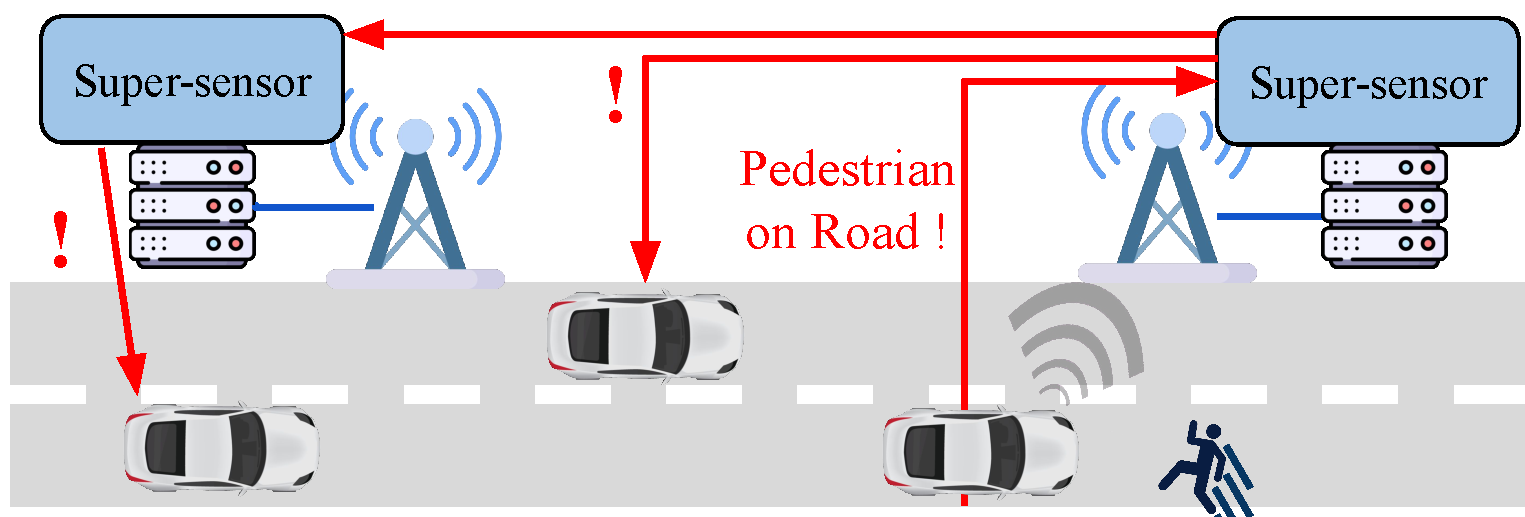
\includegraphics[width=\textwidth]{figures/apps/pedestrian}
        \caption{Detection of occluded pedestrians.}
        \label{fig:pedestrian}
    \end{subfigure}%
    ~ 
    \begin{subfigure}[t]{0.45\textwidth}
        \centering
        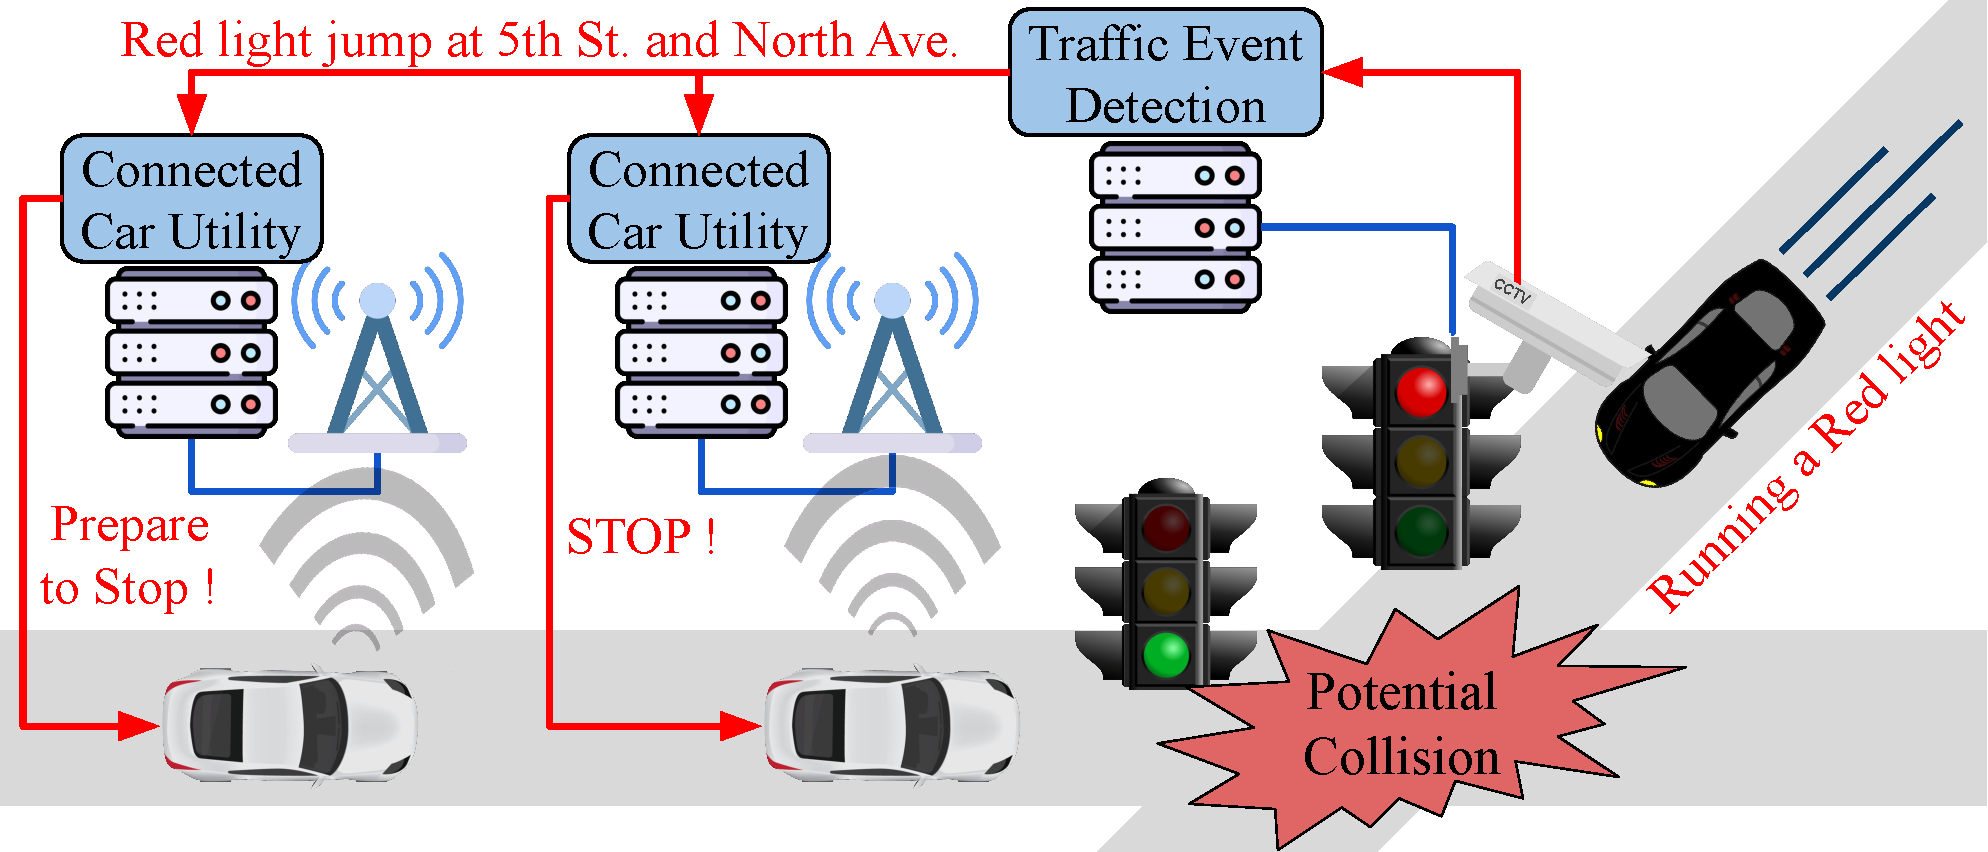
\includegraphics[width=\textwidth]{figures/apps/redlight}
        \caption{Notification of a rogue vehicle jumping a red light.}
        \label{fig:redlight}
    \end{subfigure}
    \caption{Use-cases of cooperative sensing for Autonomous driving.\todo{Add figure showing the application components as well}}
\end{figure*}
\par The fundamental components of the collaborative perception application and their functionality has been discussed and evaluated thoroughly by previous work\cite{fcooper, fusioneye, avr}. We base the application design presented here on the F-Cooper \cite{fcooper} work done by Chen et al. Each vehicle is associated with a per-vehicle application component that processes raw sensor data perceived by local on-board sensors of that vehicle and extracts features about detected objects and their location with respect to the global coordinate space.  The per-vehicle components corresponding to the set of physically close-by vehicles send streams of detected features to a fusion component. The fusion component performs feature matching among the objects reported by each per-vehicle component and de-duplicates  multiple views of the same object. Through this de-duplication process, the fusion component merges the views of multiple close-by vehicles.  Each vehicle is only interested in fused data corresponding to an area within roughly 600 meters from the vehicle's current location\cite{talkycars}. Thus a subset of the fused view is then sent back to each per-vehicle component, which relays it back to the vehicle - either to be displayed through a Heads-up Display (HUD) or for making navigation decision (in the case of autonomous vehicles).
\par The compute requirements of the fusion component is non-trivial \cite{fusioneye}, which necessitates multiple instances of the sensor fusion component serving vehicles distributed throughout a city. Boehme et al. \cite{talkycars} propose such a distributed architecture of the collaborative perception application, wherein the geographical space that the application serves is partitioned into several "regions" and all vehicles present in a specific region are served by the same fusion component. The division of a geographical space (e.g., a city) into regions is done so as to ensure uniform load distribution across the fusion components, however, that is out of the scope of this thesis.\footnote{Such a division can be done by taking into account historical levels of vehicular activity across space and ensuring that each region manager serves roughly uniform number of vehicles.} In addition to the per-vehicle object features from the vehicles present in its region, each fusion component also receives fused data from geographically neighboring regions. The data from neighboring regions allows the fusion component to serve vehicles that are close to the periphery of its region, since the 600 meter \textit{area-of-interest} of those vehicles might extend beyond the region's area. 

\par The collaborative perception application continuously ingests data perceived about the physical environment in proximity to the vehicle client, processes it and returns the result back to the client at machine-perception speed. The response-time of this sense-process-actuate control loop needs to be very small so that the driver or autonomous driving agent can react to obstacles etc. in real-time. The application involves collaboration between multiple clients, which are necessarily located in physical proximity to one another. It also requires coordination between fusion components that serve neighboring regions. This is because the area-of-interest of multiple clients which are close to each other overlap. Vehicles are inherently mobile, which creates dynamism in the compute and network requirements of the application, as well as the set of clients that are served by a given fusion component. 

\subsection{Collaborative Navigation Control in UAV Swarm}
The limited range of cameras on an individual Unmanned Aerial Vehicle (UAV) makes it cumbersome to perform large-scale jobs such as traffic monitoring or search and rescue. However, given the low cost of UAVs and the availability of communication infrastructure, using a swarm of UAVs for this purpose makes the job much easier. Swarms of UAVs have been proposed to be used for road traffic monitoring \cite{huang2021decentralized}, search and rescue \cite{scherer2015autonomous} and surveillance \cite{meng2015skystitch}. The drones that are a part of the swarm need to navigate together in order to perform a task. For instance, in the case of road traffic monitoring, drones need to coordinate among themselves so that cover the entirety of the road segment they are monitoring, while also avoiding collisions with obstacles such as poles or bridges, and other drones. In the following discussion, we will take up the use-case of road traffic monitoring to describe the application. However, the concepts generalize to other use-cases of this application.

\begin{figure}[h]
\centering
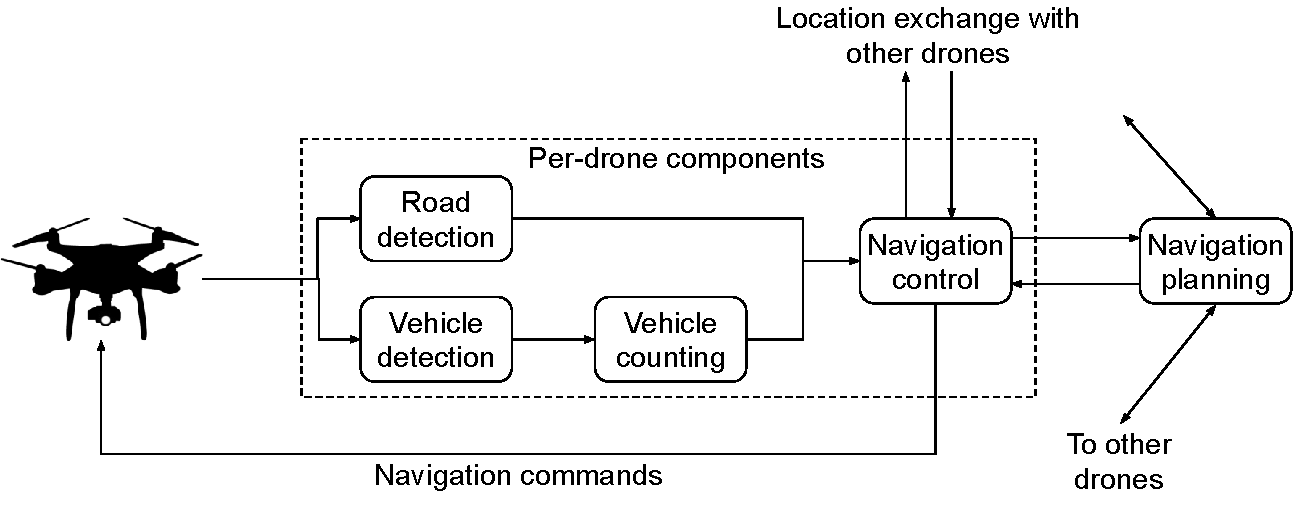
\includegraphics[width=0.75\columnwidth]{figures/apps/collab_drone_navigation}
\label{fig:collab_drone_navig}
\caption{Schematic of the Collaborative UAV Navigation application.}
\end{figure}

\par Each drone is associated with a per-drone application component, which processes the sensor data from the drone's onboard sensors. The per-drone component extracts relevant information from the sensor stream, such as vehicle counts. The extracted information is communicated to the navigating planning component, which determines whether the drone should remain in the current region of the road segment, or start monitoring another region. Drones also communicate among themselves by sharing location updates and information about detected obstacles so that they can perform fine-grained navigation control.

\par The collaborative navigation control application for drone swarms contains a real-time sense-process-actuate control loop, which continuously ingests sensor data about the physical environment. It involves coordination with other nearby drones along with having constant mobility of the clients (which are drones themselves in this case).


\subsection{Collaborative PTZ Tuning in a Distributed Camera Network}
Smart cities are seeing CCTV cameras installed at a large number of locations to record and analyze unexpected events such as accidents, crimes, etc. However, surveillance using CCTV cameras is largely done after an incident has occurred and the static deployment of cameras makes it difficult to fully capture the target objects. Contemporary cameras are often equipped with Pan-Tilt-Zoom tuning capabilities which allow them to better track target objects. Furthermore, due to the high density of cameras, they can also work collaboratively in tracking multiple target objects \cite{matsuyama2002real}.
\begin{figure}[h]
\centering
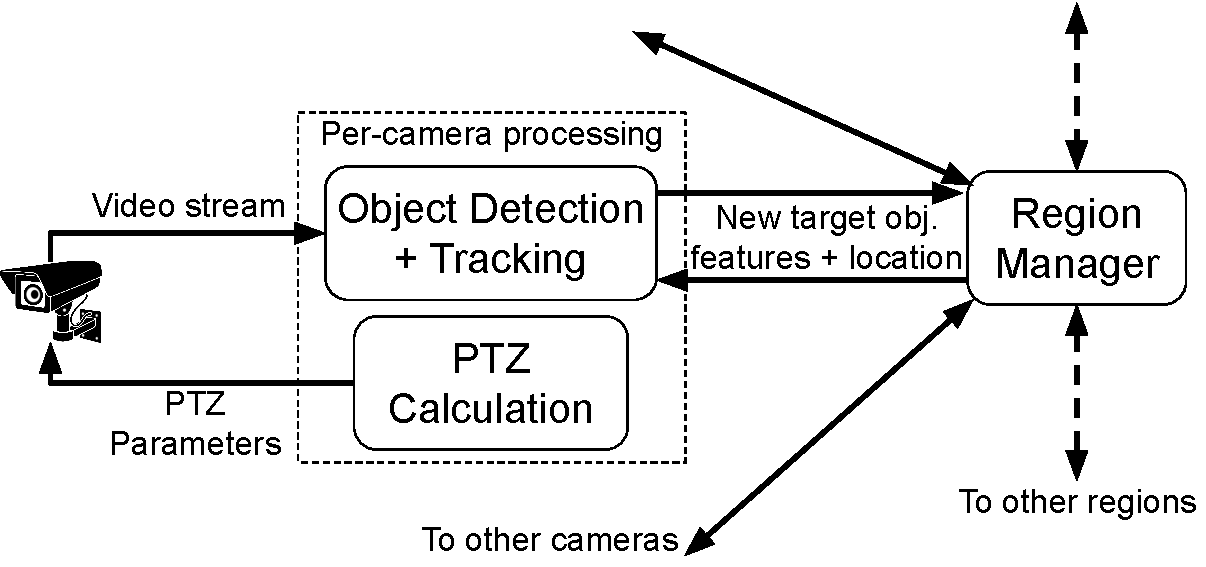
\includegraphics[width=0.75\columnwidth]{figures/apps/multi_cam_ptz}
\label{fig:multi_cam_ptz_app}
\caption{Schematic of Collaborative PTZ Tuning application for a Distributed Camera Network.}
\end{figure}
\par In order to achieve this vision, the cooperative vision application groups cameras into multiple regions and splits the application logic between a per-camera component and a per-region Region Manager (see \cref{fig:multi_cam_ptz_app}). The per-camera processing component performs object detection and tracking and informs the region manager about the features of newly detected target objects and the current location of tracked target objects. It continuously tracks target objects by adjusting the PTZ parameters. The Region Manager consumes the current location of each target object and determines the assignment of camera to target object. In case a target object is about to leave the given region, the region manager informs the neighboring region(s) of the impending arrival of the target object.
\par The collaborative PTZ tuning application requires the processing of incoming video streams in real-time to determine PTZ tuning actions. It also experiences temporal fluctuations in workload depending on the density of vehicles in each camera's field of view, which varies significantly during the day. Furthermore, multiple region-level components coordinate among each other to perform vehicle tracking over large geographical areas.

\section{Application Model}
Having described the exemplar situation-awareness applications, we now abstract out the details of each application and try to model this class of applications. We characterize the applications in terms of their compute architecture, communication patterns, storage behavior and their functionality being tied to spatial context. We discuss each of these concepts in this section.

\subsection{Computation}
\label{sec:app_model_compute}
The compute model of our target applications comprise of two main components.
\begin{itemize}
\item \textbf{Per-client component} for client-specific computation. This component is responsible for processing information generated by each client (e.g., an autonomous car or UAV) and providing input to higher layers of the application. The per-client component is specific to each application client and maintains the client's state.
\item \textbf{Region-level component} for combining information extracted from each client. Each region-level component is assigned a number of clients based on their geographical location. A given region-level component hosts  coordination and collaboration tasks between all the clients mapped to it. In the event that coordination between two clients belonging to two different regions is required, their two corresponding region-level components communicate between each other and share information.
\end{itemize}
%The compute requirements of the per-client component depends on the amount of activity perceived by the given client. Similarly, the compute requirements of a region-level component depends on the number of per-client components mapped to a it, and the workload generated by them. 
\subsection{Communication}
\label{sec:app_model_comm}
Communication among application entities in our target applications follow two primary patterns.
\begin{itemize}
\item Communication between the per-client component and region-level component. Clients share data with the corresponding region-level component for inter-client coordination and data-sharing within the region. Clients receive region-level information extracted from multiple clients. For example, in the collaborative PTZ tuning application, the per-camera component shares the current position of target objects currently assigned to it with the region manager, while receiving the locations of newly assigned target objects for it to track.
\item Area-of-Interest (AoI) based communication from a region-level component to per-client instances or other region-level components. A particular data-item is expected to be received by an application component if the data-item represents an object or event that falls within the receiver's AoI. This communication pattern can manifest itself in three ways: (1) region-level component to per-client component, as in the cooperative sensing application for autonomous driving, wherein a given vehicle receives the fused worldview not only from the region manager of the current region, but also from regions that overlap with the vehicle's area-of-interest. (2) across clients which fall in each other's AoI, as in the collaborative collision avoidance module of the UAV swarm application, which requires that UAVs share their current location among each other so that they can be aware of other UAVs in their vicinity. (3) communication between region-level components for sharing information at the region level. For instance, in the collaborative PTZ tuning application, region managers share details about a target object that is about to leave one region toward to other.
\end{itemize}
\subsection{Storage}
Applications generate state about application execution and information sensed from the environment, which needs to be persisted to enable future queries. Examples of such state include the assignment of target objects to PTZ cameras, semi-permanent road closures or traffic incidents in the collaborative driving application, etc. Such state if often tagged with the geo-location of the entity that it is describing, which is useful for executing range queries on geographical area. Data items in application's state are often read/updated by multiple entities. Applications expect a diverse set of  consistency guarantees on data access based on their application logic and reliance on most recent version of data.

\subsection{Spatial Affinity}
Since the target applications interact with the physical environment, actions taken by the application logic are often dependent on events and information from the immediate physical proximity. Hence, both computation and communication patterns of the target applications exhibit spatial affinity. Spatial affinity is defined by the Area-of-Interest of application clients and components, which represents the spatial area wherein other entities that the given entity directly interacts with are present. For instance, in the collaborative driving application, the area-of-interest of a car contains all other objects in vicinity of the car whose position information is needed in real-time to avoid potential collisions. Spatial affinity plays an important role in all facets of the application.
\begin{itemize}
\item \textbf{Computation. }Clients in physical proximity to each other are likely within each other's area-of-interest, and hence are grouped together and served by the same region-level application component. 
\item \textbf{Communication. } Communication patterns of the target applications is guided by spatial affinity of clients. Each client communicates with other clients and region-managers that fall within or overlap with the given client's area-of-interest. 
\item \textbf{Storage. }The state maintained and accessed by a application component pertains to objects and events in the subset of the physical environment that the application interacts with, and hence in physical proximity.
\end{itemize}

\section{Functional Requirements}
The target applications present a set of functional requirements on the underlying infrastructure. 
\begin{itemize}
\item \textbf{Low latency requirement. } The sense-process-actuate control loop of situation-awareness applications needs to be processed with end-to-end latency under the application's predefined threshold. This requirement ensures that the clients are able to respond in real-time to changes in the physical environment.
\item \textbf{Dynamic reconfiguration due to mobility. } Clients are continuously mobile, leading to changes in the network routes between the client devices and application components, which can result in a violation of the end-to-end latency threshold. Hence, the placement of application components needs to be adapted based on client's mobility to meet the latency requirements of the application. In addition to latency-driven reconfiguration, the mapping of per-client to region-level components needs to be reconfigured based on the current location of clients, so that inter-client coordination and data-sharing is done only between clients that are in geographical proximity of each other.
\item \textbf{Dynamic reconfiguration due to changing workload.} The workload experienced by application components (both per-client and region-level components) varies over time due to changing environmental conditions (e.g., changing number of cars detected by drones). This results in under- and over-utilization of allocated resources. Given the scarcity of edge resources and the need to continuously satisfy end-to-end latency requirements, the allocation needs to be updated so that performance requirements can be met without under-utilization of edge resources.
\end{itemize}
\section{Platform Services needed and Functional Requirements}
The aforementioned target applications can be implemented using a combination of platform services. Platform services provide the necessary systems support with powerful semantics for the applications, so that the developers can focus on the core application logic.

\subsection{Compute Orchestration}
The target applications comprise of multiple distributed components, each with a specific functionality. These application components require appropriate resource allocation to cater to their specific computational requirements such that a low sense-process-actuate control-loop latency can be ensured. Furthermore, for the application's correctness, per-client components should be mapped to the right region-level component based on client's current location. This problem is further complicated by the mobility of clients. Client mobility necessitates the dynamic reassignment of per-client components to region-level components because the set of clients present in a given region keeps changing over time. Furthermore, the spatial distribution of clients varies with time, and therefore the workload at each application component. This necessitates dynamic updates to the resource allocation of application components to avoid under-utilization or over-utilization of resources. 
\par Compute orchestration platform service handles all the above issues without requiring the developer's intervention. Given the latency and spatial affinity requirements of applications, the platform service will automatically deploy and reconfigure the resource allocation and connectivity of application components. Detecting the need for a reconfiguration entails continuously monitoring the end-to-end latency of the application's sense-process-actuate control-loop and mobility of clients and checking if a violation of latency or spatial affinity occurred. Once a violation is detected, the application orchestrator reconfigures the application instance, either by updating resource allocation in the case of over or under-utilization, or by updating the client-to-application component mapping in the case of spatial affinity violation.

\begin{comment}
To ensure correct functionality of sense-process-actuate control loop, applications need to be deployed on edge sites to ensure that the end-to-end compute latency constraints imposed by the applications are satisfied. End-to-end latency refers to the total time taken to process a data item by all the application components from the time when it is generated by a client. End-to-end latency is not just a function of compute latency at each application component, but also the network latency between components - which in incurred to communicate the processing result of an upstream component to the downstream component. Hence, in addition to the amount of resources allocated to each application component on edge sites, the selection of the edge sites for hosting application components and network latencies between them  affects end-to-end latency. Furthermore, to serve the spatial affinity requirements of applications, per-client components need to be mapped to the right region-level component, so that data sharing can be done effectively. 
\par Clients are continuously mobile, which affects network latency between the client and the per-client application component, thereby affecting the end-to-end latency of the application. Moreover, mobile clients tend to frequently change the geographical regions that they belong to, which makes data sharing through their current region-level component ineffective. Hence, the placement of application components and the mapping of per-client component to region-level component needs to be dynamically updated to ensure continuous latency and spatial affinity satisfaction. Doing so also relies on monitoring the location of clients and experienced network latencies between clients and application components and detecting violations.
\par Dynamically managing application components of a large number of clients over a heterogeneous edge infrastructure is challenging for application developers. Hence, compute orchestration is a key platform service that reduces the burden of application developers by making sure that the application-specific requirements of latency and spatial affinity are satisfied. 
\end{comment}
\subsection{Publish-Subscribe Communication}
The communication patterns in the target situation-awareness applications ranges from one-to-many (region-level component to per-client component), many-to-one (per-client component to region-level component) and many-to-many patterns (among clients). Furthermore, given the continuous mobility of clients and the dependence of communication pattern on spatial affinity, the set of entities communicating with a given client changes over time. Implementing the communication subsystem for a given application would require maintaining a dynamically updated list of receivers for each data sender, ensuring reliable message delivery to all receivers, etc., which are challenging for application developers.
\par Publish-subscribe is a useful communication model, which uses the abstraction of "topics" to define interaction between entities. Special nodes called "brokers" host topics and perform message transfer from producers to consumers of each topic. The use of intermediary broker nodes allows the producers and consumers to be decoupled from each other. Data producers can send messages to a topic without waiting for it to be received by consumers, and consumers are notified asynchronously for each message. Publish-subscribe systems also maintain a persistent log of messages for each topic, which allows them to ensure strong data-delivery semantics, such as atleast-once delivery of messages to each consumer.

\subsection{Key-Value Storage}
The processing logic of our target applications depend on their state, hence it should be stored in a way that facilitates easy and efficient access. Key-value stores offer a convenient data model, wherein each data-item can be referenced using a unique key for reading and writing. Typically, key-value stores maintain multiple replicas of each data-item to ensure tolerance from failures. The network connectivity of data replicas and the number of replicas chosen for performing a read or write operation determines the operation latency and the consistency. Supporting a diverse set of applications with different latency and consistency guarantees requires that replica selection takes into account both the requirements of the application as well as the infrastructure topology.

\section{Timing considerations for situation-awareness applications}
\subsection{Why cloud-based solutions fall short?}
A number of platform services offering compute orchestration (e.g., Kubernetes), publish-subscribe communication (e.g., Apache Pulsar) and key-value storage (Apache Cassandra) are available for the cloud computing ecosystem. These services are widely used since they provide strong data-plane semantics (such as Cassandra's tunable consistency levels and Pulsar's at-least-once message delivery guarantee). In addition to useful semantics, the data-plane of these systems have been tuned for providing high throughput and low latency. 
\par However, relying on cloud-based solutions necessitates communicating with a remote datacenter location through the wide area network (WAN), and sending all of the data from client's sensors to the datacenter. Traversal through the WAN incurs high and unpredictable communication latency, and the large volume of high-fidelity sensor data (e.g., stereo cameras, LiDAR, etc.) causes high backhaul bandwidth consumption. 

\subsection{Need to move to the network edge}
Edge computing \cite{edge} presents a viable deployment alternative for the aforementioned platform services. The presence of computation and storage resources in proximity to the clients makes it possible reduce the network latency between the clients and application components. Edge infrastructure is a continuum of geo-distributed \emph{sites} hosted by multiple providers, such as telecommunication network providers, co-location providers (e.g., Vapor IO \cite{}), etc. An edge site typically comprises of a rack of server-grade machines, equipped with storage and networking infrastructure. Edge infrastructure has a wide geographical coverage in order to provide low-latency access to a large number of users. The wide geographical coverage coupled with heterogeneous connectivity results in non-trivial communication latencies between edge sites.  
\subsection{New mechanisms are needed at the edge}
The cloud-based platform services don't offer the same performance when deployed as-is on edge infrastructure because their control-plane policies are not optimized for an edge setting. These systems have been designed for operating in a datacenter setting, wherein machines are connected to each other via a high-throughput low-latency network. Clients, compute and data entities are co-located in the same datacenter, making the network latencies between these components negligible as compared to the compute and data access latencies. Hence, in these systems, the key to ensuring bounded end-to-end latency is uniform load balancing that prevents the formation of workload hotspots and therefore latency inflation. Using such systems as-is in an edge computing environment would result in the placement of compute and data entities on edge sites in a way that is agnostic of network latencies between edge sites - making the satisfaction of end-to-end latency requirements difficult. Furthermore, cloud-based platform services don't monitor observed end-to-end latencies to detect a violation and trigger reconfiguration.
\par In order to better serve the target applications, we need to introduce new edge-specific mechanisms into the control-plane of the platform services. Doing so will allow them to operate effectively in an edge setting and meet the requirements of applications.
    \chapter{Necessary Mechanisms for Geo-Distributed Operation of Platform Services}
\begin{comment}
How to realize platform services at the edge?
    - describe core mechanisms needed
    - discuss how these mechanisms will enable efficient implementation of the aforementioned platform services in geo-distributed edge infrastructure
    - discuss the conceptual relationship of these mechanisms to the state-of-the-art in the cloud and other related research works
\end{comment}

\section{Introduction}
The challenges imposed by the peculiar characteristics of a geo-distributed Edge infrastructure and situation-awareness applications on the control-plane design for platform services necessitate the introduction of novel mechanisms to address them. We propose three key mechanisms in this dissertation to address these challenges - Dynamic Spatial Context Management, Network Proximity Estimation and End-to-End Application Monitoring. 
\par The Dynamic Spatial Context Management mechanism allows the control-plane of platform services to maintain a frequently updated view of the spatial context of system entities such as application instances, data-items and end-clients. This spatial context information is used to make control-plane policy decisions, such as mapping a client to an application instance, determining the set of clients that need to share data for inter-client coordination, etc. The objectives of these control-plane policies is to ensure that the spatial affinity requirement of an application is fulfilled. \todo{Introduce spatial affinity requirement in previous chapter and point to it.} 
\par While the Dynamic Spatial Context Management mechanism is used to establish logical connectivity between system entities based on spatial proximity, it is not responsible for mapping those system entities on to the physical infrastructure - a problem that requires knowledge of infrastructure topology heterogeneity and latency requirements of applications to be kept in mind. The Network Proximity Estimation mechanism allows control-plane policies to estimate the network latency between physical nodes in the infrastructure which can be used for the placement of system entities such that applications' requirements are satisfied. 
\par Finally, the continuous execution of applications requires the control-planes of platform services to monitor the end-to-end latency experienced by each application instance, which includes queuing and computation delays as well as communication delays between different entities. The End-to-End Monitoring mechanisms allows the control-plane policies to obtain an aggregated view of the various component latencies making up the end-to-end observed latency so that the policies can detect a violation of the application's requirements. The end-to-end view of observed latencies also enable a root-cause analysis to identify the source of the performance violation and trigger the appropriate reconfiguration action to alleviate it. 
\par In this chapter, we will discuss the three mechanisms proposed in this dissertation in detail. We first present the infrastructure and workload scenario that has been considered to motivate the problems solved by these mechanisms and to design the experimental settings. Then, for each mechanism, we will first describe the objective of the mechanism, enumerate examples of control-plane policies that will benefit from it, present the abstractions exposed to the control-plane policies, and why previous approaches at attaining this objective are not sufficient. Finally, we demonstrate the use of these abstractions for building useful control-plane policies that can support the efficient operation of platform services on a realistic Edge infrastructure against a workload of situation-awareness applications. 

\subsection{Infrastructure Topology and Client Workload considered}
\label{sec:nep_infra_topology}
\par To make the case for the mechanisms proposed in this dissertation, we utilize the dataset released by a previous work \cite{xu2021cloud}. The dataset characterizes the Edge cloud service of Alibaba Cloud, both at the infrastructure and workload level. At the infrastructure level, it provides detailed information about the number of edge sites in each city and the network provider who owns them, the number and size of physical machines in each edge site and the network round-trip time between sites. At the workload level, the dataset contains information about the number and size of VMs hosted by each physical machine and the CPU utilization of each VM. For this evaluation, we focus on the city of Shanghai. We simulate client activity (including mobility) in the city of Shanghai, and thus to determine the network connectivity between a client and Edge site, it is important to know which cell towers are served by a given Edge site, or in other words, the geographical coverage of each Edge site. To estimate the coverage of each Edge site, the precise geographical location of Edge sites and their connectivity with cell towers is needed. However, the dataset only provides a city-level granularity of Edge site locations. Hence, to estimate their precise geo-location, we gather the locations of cell towers owned by the different network providers from CellMapper \cite{cellmapper}, perform k-means clustering on them and obtain the likely location of the edge sites. The number of k-means clusters for each network provider's cell tower clustering is made equal to the number of Edge sites owned by that provider in Shanghai (from the dataset). Upon obtaining the locations of Edge sites using clustering, we need to assign resource capacity to each site. For this we again use the Alibaba Edge Node Service dataset, which contains information about the resource capacity of each Edge site. To map the resource capacity from the dataset to an Edge site location extracted via clustering, we assigns the most resource-rich site's resources capacity in the dataset to the Edge site location that has the maximum number of cell towers in its cluster, and so on. \cref{fig:shanghai_infra} illustrates the infrastructure topology, with the locations of cell towers and Edge sites marked. In addition to Edge site within Shanghai with fine-grained locations, the physical infrastructure considered also consists of Edge sites in other cities of China. Each Edge site outside Shanghai is significantly farther away from any client considered in the workload (compared to sites within Shanghai), and therefore its precise location is set to be the center of the city that it is located in.

\begin{figure}
\centering
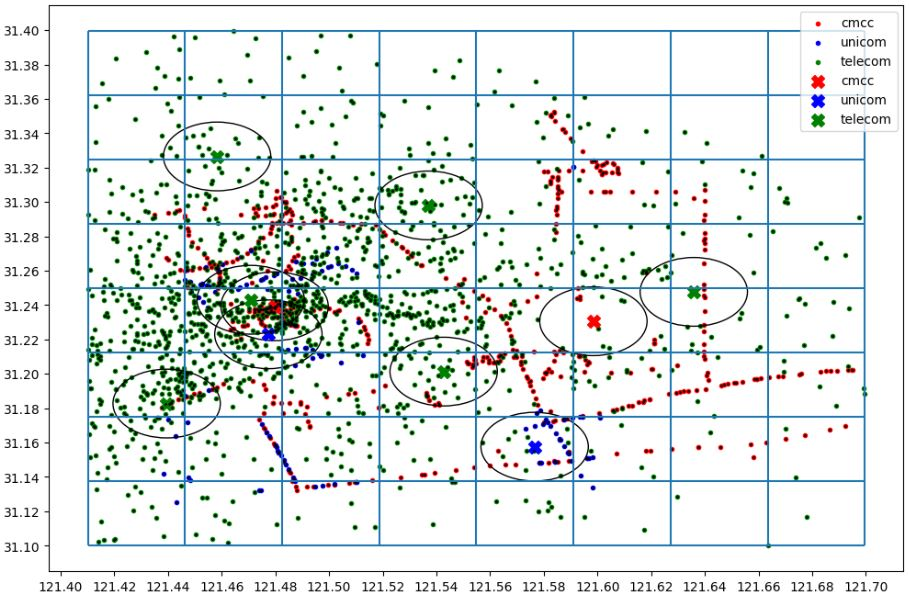
\includegraphics[width=0.5\textwidth]{figures/mechanisms/shanghai_infrastructure.JPG}
\caption{Edge infrastructure of the city of Shanghai which is under consideration in this chapter. The crosses denote Edge site locations, while the dots denote cell towers. \todo{Add lat-lng to the axes labels. Update the legend to be more meaningful.}}
\label{fig:shanghai_infra}
\end{figure}

\section{Dynamic Spatial Management Mechanism}
\label{sec:spatial_ctx_mgmt}

Situation-awareness applications, e.g., collaborative autonomous driving and UAV swarm navigation, interact with the physical environment, by sensing environment data and performing actions on it. Typically, there are many clients of the same application operating in a common geographical space. In such a setting, a client's processing logic can benefit by incorporating information extracted from other clients' sensed data. For a given client, the set of other clients that it needs to coordinate with depends on the location of clients, the size of their sensor range and the area of interest of the given client. The area of interest (AoI) of a client is defined as the geographical region about which it is interested in receiving information. The sensing range of a client depends on the sensor hardware used, e.g., LiDAR or camera. The size of the Area-of-Interest depends on the nature of the application. For instance, since vehicles in a city are not expected to move at speeds higher than , say, 25 miles per hour (in urban cities in USA), the size of AoI of vehicular clients for the collaborative perception application is bounded \todo{Add number from TalkyCars paper}. There exists only a finite region around a given vehicle that would contain any interesting event for the vehicle.
\begin{figure}
\centering
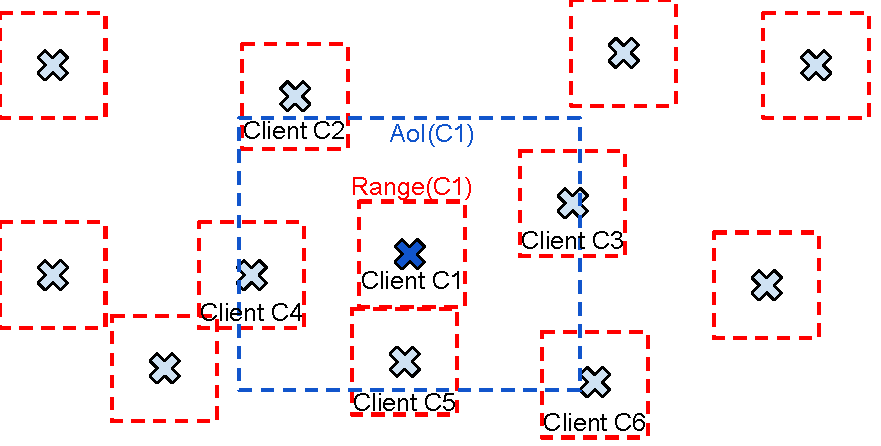
\includegraphics[width=0.75\textwidth]{figures/mechanisms/spatial_ctx_mgmt/aoi_range.pdf}
\caption{An exemplary spatial distribution of situation-awareness application clients overlaid on two-dimensional space. The sensing range of clients is shown as a red dashed rectangle around the client's location. The Area-of-Interest of client C1 is shown.}
\label{fig:aoi_range}
\end{figure}
\cref{fig:aoi_range} shows a typical arrangement of clients in geographical space with the sensing range of each client marked in red and the AoI of one of the clients C1 marked in blue. Each client senses data from the environment within its range and the application instance serving it generates actionable information from the sensed data. Client C1's application instance is interested in receiving all actionable information about the subset of environment within its AoI's bounding-box. Hence, C1's application instance needs to interact with all other application instances that are serving those clients whose range bounding-box overlaps with the AoI bounding-box of C1. 

\begin{figure}
\centering
\begin{subfigure}{0.45\textwidth}
  \centering
  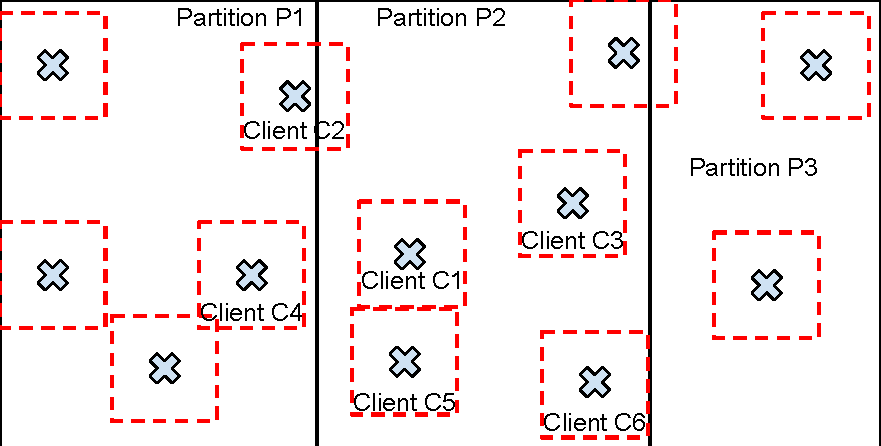
\includegraphics[width=\linewidth]{figures/mechanisms/spatial_ctx_mgmt/aoi_range_partition.pdf}
  \label{fig:aoi_range_partition}
  \caption{The partitioning of geographical space. Each partition is to be managed by a distinct application component. The important point to note is that each partition is not self-sufficient, but rather relies on information from other partitions as well. This is because the AoI of clients inside a given partition overlaps with the range of clients in other partitions.}
\end{subfigure}%
~~~
\begin{subfigure}{0.45\textwidth}
  \centering
  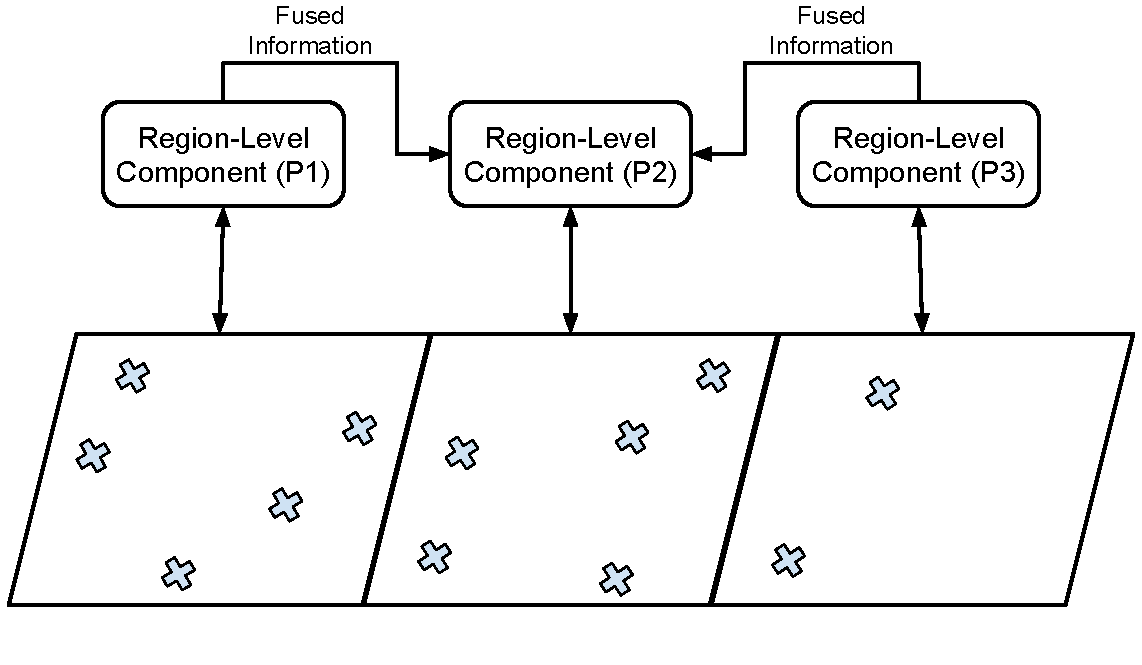
\includegraphics[width=\linewidth]{figures/mechanisms/spatial_ctx_mgmt/aoi_range_partition_mapping.pdf}
  \caption{Clients in each spatial partition are mapped to a unique region-level component that is responsible for fusing the information extracted from each individual client.}
  \label{fig:aoi_range_partition_mapping}
\end{subfigure}
\caption{Illustration of partitioning of geographical space to support large-scale deployment of situation-awareness applications that require coordination among clients.}
\label{fig:spatial_partitioning}
\end{figure}

An intuitive way of modeling these applications was discussed in \cref{sec:app_model_compute}, wherein a region-level component is responsible for fusing the information extracted from multiple clients to realize inter-client coordination. However, in a large-scale geo-distributed deployment of such applications, a single region-level component would be insufficient to serve all the clients - because of scalability limitations of the fusion application component, resource constraints on the Edge site hosting it, or both \cite{talkycars}. Hence, to support a large number of clients, multiple instances of region-level component are maintained as shown in \cref{fig:spatial_partitioning}, with each instance serving a distinct partition of the entire geographical area. All clients within a given spatial partition should be served by the same region-level instance, thus enabling inter-client coordination among all clients within that partition. Due to the inherent mobility of clients and the fact that the spatial partitioning is not necessarily aligned with the range of each client, a client's AoI can overlap with another client's range that is located in a different partition. For example, in \cref{fig:aoi_range_partition} client C1's AoI overlaps with the range of client C4, however C1 and C4 belong to partitions P2 and P2 respectively. To make sure that information from client C4 is taken into account while processing the sensor data of client C1, the region-level component instance serving client C1 receives a stream of fused information from the instance serving client C4, as shown in \cref{fig:aoi_range_partition_mapping}. 

\par For situation-awareness applications that require inter-client coordination \todo{Check if introduced in previous chapter}, mapping clients to region-level component instances needs to be done by taking into account the spatial context of clients (denoted by their location) and that of the region-level instances (denoted by spatial partition they are meant to serve). Information sharing between region-level instances is also dictated by the spatial context of the different instances and the range and AoI of clients served by those instances, as shown in \cref{fig:spatial_data_sharing}. 

\begin{figure}
\centering
\begin{subfigure}{0.4\textwidth}
  \centering
  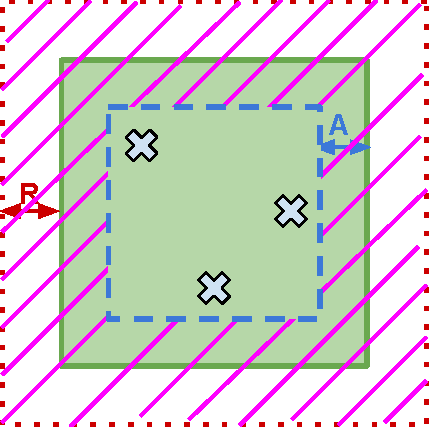
\includegraphics[width=\linewidth]{figures/mechanisms/spatial_ctx_mgmt/out_data.pdf}
  \label{fig:spatial_ctx_out_data}
  \caption{An illustration of the information generated by a given region-level component instance that needs to be shared with other instances.}
\end{subfigure}%
~~~
\begin{subfigure}{0.4\textwidth}
  \centering
  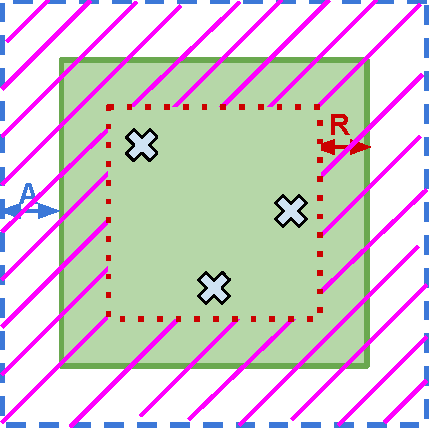
\includegraphics[width=\linewidth]{figures/mechanisms/spatial_ctx_mgmt/in_data.pdf}
  \caption{An illustration of the information needed by a region-level application component from other application instances. }
  \label{fig:spatial_ctx_in_data}
\end{subfigure}
\caption{The shaded regions in both images show the data which needs to be shared with other region-level instances (\cref{fig:spatial_ctx_out_data}) and which needs to be received from other instances (\cref{fig:spatial_ctx_in_data}). The $R$ denotes the size of sensing range, while $A$ represents the size of AoI of each client. \todo{Need to say that the shaded area represents area for all possible client locations within the partition. It is not specific to a certain client location.}}
\label{fig:spatial_data_sharing}
\end{figure}
Thus, to ensure that each client is served by an application instance specific to its spatial context and that application instances are able to share relevant data among each other, it is imperative to treat the spatial context of clients, application components and data-items as first-class attributes. 
\par The main challenge in doing so is to handle continuous client mobility, which results in the AoI and spatial context of each client to change continuously. Hence, a static mapping of clients to application instances would result in frequent violation of spatial affinity \todo{What is a violation should be mentioned before}. Furthermore, given the continuous mobility of clients and the limited resource capacity of edge resources, workload skews are much more common - caused due to a large number of clients accumulating in a particular partition, e.g., in the event of a surge in vehicular traffic in a city's downtown area due to a concert. Such spatial workload skews would necessitate the monitoring and remapping of geographical regions to applications instances and data-items, so that the skews can be minimized and performance hotspots can be avoided.

\subsection{Control-plane actions that need this mechanism}
The are two main actions taken by the control-planes of platform services which require spatial context information of clients and compute and data components.
\par \noindent \textbf{Dynamic Client-Application Mapping. } Situation-awareness applications require that a client be connected to a region-level application component instance that is assigned to the spatial area within which the client is currently located. A metric that quantifies the goodness of this mapping is Spatial Alignment, which measures how many of the expected clients that should have been mapped to an application component are actually mapped. The metric for spatial area $A$ is quantified in \cref{eq:spatial_alignment}.
\begin{equation}
SA \left( A \right) = \dfrac{\text{max. clients in }A\text{ served by the same app instance}}{\text{number of clients in }A}
\label{eq:spatial_alignment}
\end{equation}
The control-plane policy for client-application mapping would ideally ensure the spatial alignment metric for all spatial areas is 1.0, meaning that all clients that are currently located in a given spatial area A are connected to the same application instance.

\par \noindent \textbf{Area-of-Interest Queries. } Clients and application components need to query data-items whose spatial context overlaps with the querying entity's AoI. This query is served by the control-plane which evaluates the spatial context overlap with querying entity's AoI and returns a list of satisfying data-items. We use a metric called AoI Satisfaction Rate to quantify the goodness of the query, as shown in \cref{eq:aoi_sat_rate}.
\begin{equation}
\text{AoI Satisfaction Rate} = \dfrac{|\{ e: e \text{ is returned by query  and } e \in AoI \}|}{|\{ e: e \in AoI \}|}
\label{eq:aoi_sat_rate}
\end{equation}
Ideally the control-plane policy for evaluating these queries should be able to achieve an AoI Satisfaction Rate of 1.0.


\subsection{Limitations of previous work in implementing policies}
Contemporary Edge computing solutions do not allow coordination among application components that are deployed across multiple Edge sites \cite{gabriel, azure_iot_edge}. Hence, a client $c$ that is mapped to an Edge site $E$ can only coordinate with other clients that are also mapped to the site $E$. Similarly, $c$ can only discover other system entities that are connected to the site $E$. We consider 2 high-level approaches in which clients have been mapped to Edge sites in previous work - mapping clients to the geographically closest site (GeoDist) (as in \cite{lahderanta2021edge}) and to the site with smallest RTT from the client (RTT) (as in \cite{foglets}). In the following evaluations, we show how both these approaches are deficient in satisfying the spatial alignment requirement of client-to-application mapping as well as serving Area-of-Interest based queries.

\begin{figure}
\centering
\begin{subfigure}{0.45\textwidth}
  \centering
  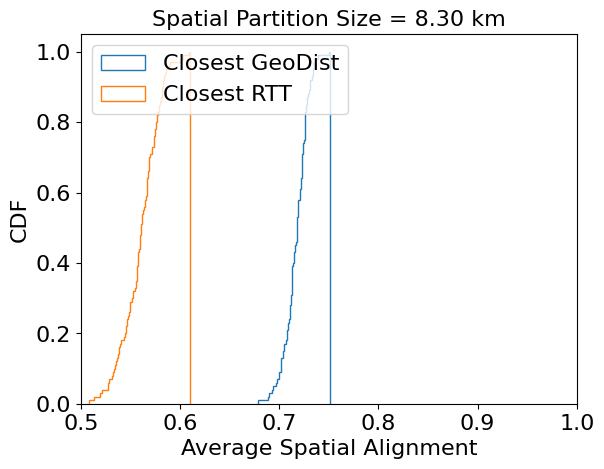
\includegraphics[width=\linewidth]{figures/mechanisms/spatial_ctx_mgmt/spatial_alignment_randomized_4_rows.png}
  \caption{}
\end{subfigure}%
\begin{subfigure}{0.45\textwidth}
  \centering
  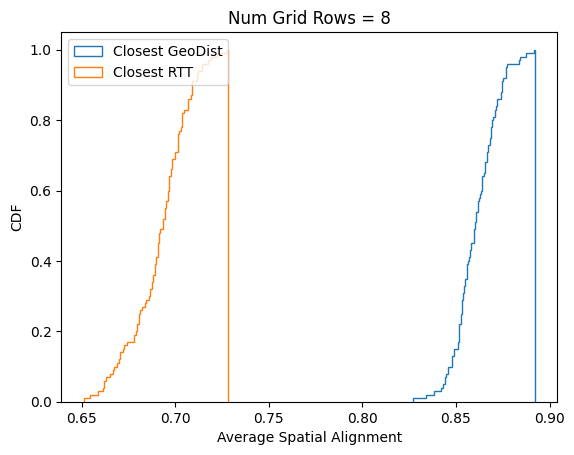
\includegraphics[width=\linewidth]{figures/mechanisms/spatial_ctx_mgmt/spatial_alignment_randomized_8_rows.png}
  \caption{}
\end{subfigure}\par\medskip
\begin{subfigure}{0.45\textwidth}
  \centering
  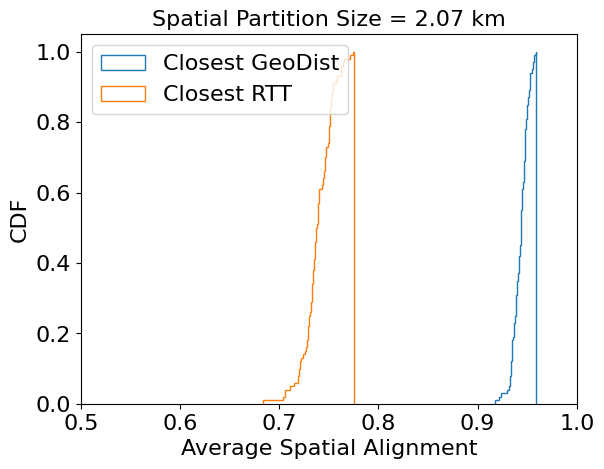
\includegraphics[width=\linewidth]{figures/mechanisms/spatial_ctx_mgmt/spatial_alignment_randomized_16_rows.png}
  \caption{}
\end{subfigure}%
\begin{subfigure}{0.45\textwidth}
  \centering
  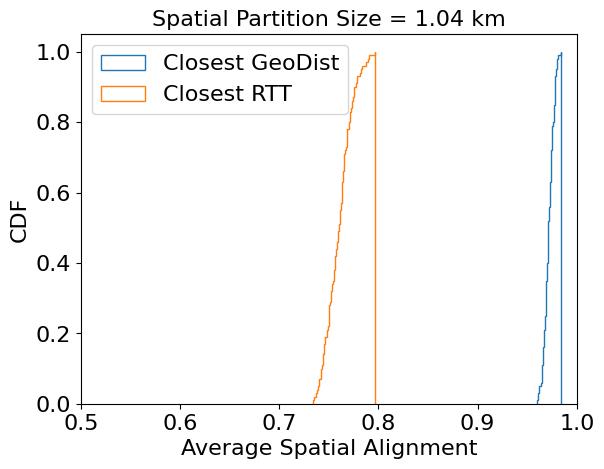
\includegraphics[width=\linewidth]{figures/mechanisms/spatial_ctx_mgmt/spatial_alignment_randomized_32_rows.png}
  \caption{}
\end{subfigure}
\caption{Distribution of Average Spatial Alignment observed for different sizes of spatial partitioning. Closest RTT based mapping of clients to Edge sites results in worse spatial alignment compared to Closest Geo Distance based mapping. \todo{Change the control knob from Num Grid Rows to Size of Spatial Partition (m)}}
\label{fig:spatial_alignment_eval}
\end{figure}

\par \noindent \textbf{Spatial Alignment Evaluation. }To evaluate the above client-to-application mapping baseline heuristics in terms of spatial alignment, we first consider the area of the city under evaluation and divide it into a number of spatial partitions, within which we ideally expect clients to be grouped and served by the same application instance (thereby creating a perfect spatial alignment). The size of spatial partitions is varied in the experiment to represent a diverse set of applications. We create 1000 clients (with equal number of clients in each network provider) and place each one of them at a cell tower location. The placement of clients at cell tower locations is justified by the fact that the spatial distribution of cell towers follows that of client activity. This client placement is randomized and the experiment is repeated 100 times. For each experiment run, we compute the average spatial alignment over all spatial partitions in the scenario. \cref{fig:spatial_alignment_eval} shows the distribution of the average spatial alignment that results from mapping clients to application instances using greedy heuristics that aim at minimizing geographical distance and network RTT between the client and Edge site. The metric shown is average spatial alignment, which is the average of the spatial alignment of all the spatial areas. Although the baseline policy GeoDist, which selects the geographically closest Edge site, is able to attain a high enough average spatial alignment, but doesn't attain the perfect 1.0 value because not all clients in a given spatial partition always have the same Edge site to be the closest. Furthermore, the Closest RTT approach offers even worse spatial alignment because in a given spatial partition, clients belonging to two different network providers are bound to be mapped to different sites. 

\begin{figure}
\centering
\begin{subfigure}{0.3\textwidth}
  \centering
  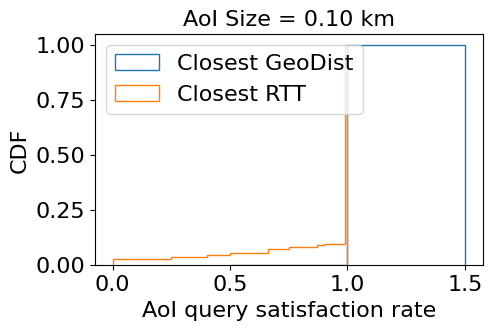
\includegraphics[width=\linewidth]{figures/mechanisms/spatial_ctx_mgmt/aoi_satisfaction_rate_cdf_AOI_0.100_km.png}
  \caption{}
\end{subfigure}%
\begin{subfigure}{0.3\textwidth}
  \centering
  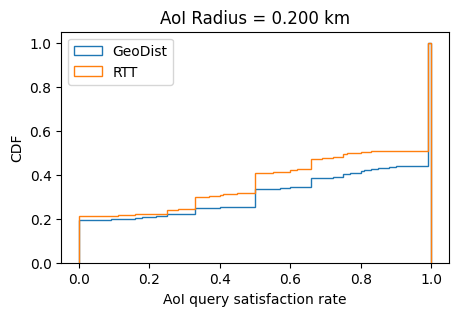
\includegraphics[width=\linewidth]{figures/mechanisms/spatial_ctx_mgmt/aoi_satisfaction_rate_cdf_AOI_0.200_km.png}
  \caption{}
\end{subfigure}
\begin{subfigure}{0.3\textwidth}
  \centering
  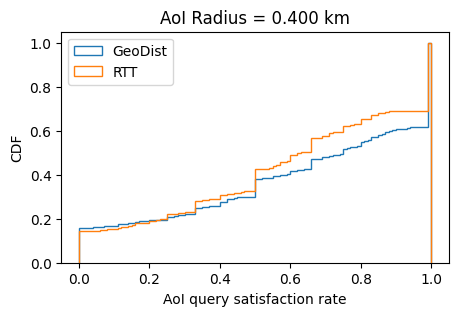
\includegraphics[width=\linewidth]{figures/mechanisms/spatial_ctx_mgmt/aoi_satisfaction_rate_cdf_AOI_0.400_km.png}
  \caption{}
\end{subfigure}
%\par\medskip
\begin{subfigure}{0.333\textwidth}
  \centering
  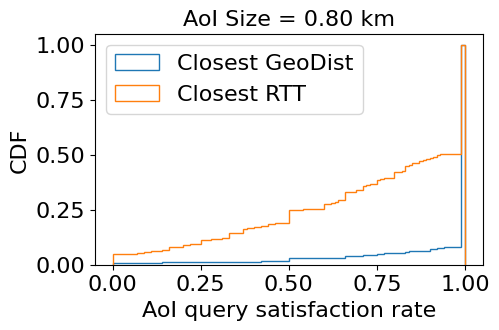
\includegraphics[width=\linewidth]{figures/mechanisms/spatial_ctx_mgmt/aoi_satisfaction_rate_cdf_AOI_0.800_km.png}
  \caption{}
\end{subfigure}%
\begin{subfigure}{0.333\textwidth}
  \centering
  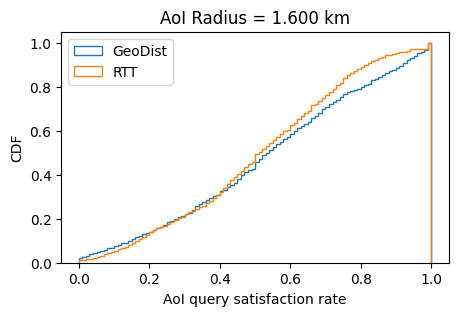
\includegraphics[width=\linewidth]{figures/mechanisms/spatial_ctx_mgmt/aoi_satisfaction_rate_cdf_AOI_1.600_km.png}
  \caption{}
\end{subfigure}%
\begin{subfigure}{0.333\textwidth}
  \centering
  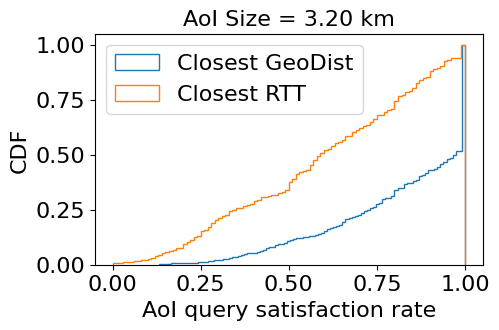
\includegraphics[width=\linewidth]{figures/mechanisms/spatial_ctx_mgmt/aoi_satisfaction_rate_cdf_AOI_3.200_km.png}
  \caption{}
\end{subfigure}
\caption{AoI Satisfaction Rate \todo{Expand this caption. Make AoI a rectangular box and not a circle with radius}}
\label{fig:aoi_satisfaction_rate_eval}
\end{figure}

\par \noindent \textbf{AoI Satisfaction Evaluation.} Next, \cref{fig:aoi_satisfaction_rate_eval} shows the distribution of AoI query satisfaction rate offered by the Closest GeoDist and Closest RTT baseline policies for retrieving the system entities with spatial context overlapping with the AoI of the querying client. For this evaluation, we create one client at every cell tower location, and each client submits an AoI query to find which other clients are in its AoI. Depending on the client-Edge-site mapping, a variable number of AoI members are returned, which is compared with the actual set of clients within the AoI to compute the query satisfaction rate. The size of AoI query is varied to represent a diverse set of applications and their satisfaction rate distributions are shown. Both client-to-application mapping approaches perform poorly and fall significantly short of the expected AoI Query Satisfaction Rate of 1.

\subsection{Interface exposed to the control-plane}
The Dynamic Spatial Context Management mechanism is utilized by both the centralized control-plane compute/data placement policy of platform services as well as the client library of the platform service running on the client application. The centralized control policy interacts with this mechanism to maintain the spatial context of the system entities (data and compute) while the client library uses this mechanism to keep track of the spatial context of clients. Both these types of spatial contexts are useful in determining which compute/data entities a given client would need to access. 
\par We divide the geographical space into rectangular regions called \textit{Tiles}, which are of arbitrary size. \todo{Why tiles? Need a reference or explanation about why tile is enough.} An example partitioning is shown in \cref{fig:aoi_range_partition}.\todo{Fix this cref} Each Tile has a unique Tile ID, which can be used to directly reference the Tile. Each tile contains a number of entities, such as clients or data-items. In the following list, we enumerate the various functions that the mechanism exposes to the control-plane for accessing and updating this partitioning.
\begin{itemize}
\item \textbf{GetTileID}. This function takes a location as input and returns the ID of the Tile inside which that location falls.
\item \textbf{GetTileCoverage}. This function takes the ID of a tile as input and returns the bounding box which represents the spatial area covered by the tile.
\item \textbf{UpdateEntityLocation}. Update the location of an entity. In addition, if the new location of the entity is in a different tile than its previous location, this function would move the entity from previous tile to the new tile. 
\item \textbf{GetIntersectingTiles}. This function takes in a bounding box and returns the set of tiles that intersect with it. This function is useful for range queries.
\item \textbf{SplitTile}. This function call is used to split a tile into two. The split is carried out in a way to ensure that the number of entities in the two resultant tiles is (almost) equal. This function is used to handle load.
\item \textbf{MergeTiles}. This function allows the control-plane to trigger a merging of two adjacent tiles.
\end{itemize}

\subsection{Demonstration of using the mechanism for implementing a control-plane policy}
We now demonstrate how the proposed mechanism and the associated API are useful in implementing control-plane policies for platform services. For this mechanism, we use an application orchestrator as the driving example. \cref{algo:deploy_req} shows the pseudocode of the control-plane policy for finding a suitable application instance for mapping a client based on its geographical location and the spatial contexts of various region-level application instances. The control-plane maintains a mapping $APPS$ between an application instance and the Tile which represents the geographical area served by the application instance. The policy first determines the Tile in which the client is currently located. If the client's tile already has an application instance associated with it, it returns connection information about that instance. Otherwise it deploys a new application instance for the client's tile, maps the application instance to the tile and returns its information to the client. The policy also adds the client to the tile to update the occupancy information, which can be used to detect overload and trigger re-partitioning.
\begin{algorithm}
\caption{Handling Deploy Request from Client}
\begin{algorithmic}
\Require client $c$
\Require client's location $loc$
\State $t \gets GetTileID \left( loc \right)$
\If{$APPS \left[ t \right] exists$}
    \State $A \gets APPS \left[ t \right]$
\Else
    \State Deploy app component $A$ for tile $t$
    \State $APPS  \left[ t \right] \gets A$
\EndIf
\State $UpdateEntityLocation \left(t, c \right)$
\State $SendConnectionInfo \left(c, A \right)$ \Comment{Send info to client for connecting to app component}
\end{algorithmic}
\label{algo:deploy_req}
\end{algorithm}

\cref{algo:handle_overloaded} describes the control-plane policy for handling an overloaded region-level component due to workload skew. This policy is triggered by the control-plane when it identifies that a given application instance is overloaded by the compute requirement of serving all the clients that are currently present in the tile its is serving. Hence, the tile needs to be split and workload divided among two application instances. The policy takes as input the tile associated with the overloaded application instance. The policy uses the \textit{SplitTile} function to create two new tiles. It reuses the application instance for the old tile for one of the new ones, and deploys another instance for the second new tile. Each client that belonged to the old tile is now a part of one of the two new tiles. The policy sends the connectivity information of the new application instances to the respective clients. Although not shown, the \textit{MergeTiles} functionality provided by the mechanism can be similarly used to merge two tiles together if the two application instances serving these two tiles are sufficiently underutilized.
\begin{algorithm}
\caption{Handling an Overloaded Tile}
\begin{algorithmic}
\Require overloaded tile $t$
\State $t1, t2 \gets SplitTile \left( t \right)$
\State $APPS \left[ t1 \right] \gets APPS \left[ t \right]$
\State Deploy app component $A$ for tile $t$
\State $APPS  \left[ t2 \right] \gets A$
\For{client $c \in GetEntities \left( t1 \right)$}
    \State $SendConnectionInfo \left(c, APPS \left[ t1 \right] \right)$
\EndFor
\For{client $c \in GetEntities \left( t2 \right)$}
    \State $SendConnectionInfo \left(c, APPS \left[ t2 \right] \right)$
\EndFor
\end{algorithmic}
\label{algo:handle_overloaded}
\end{algorithm}

\section{Network Proximity Estimation}
The performance perceived by applications when using platform services heavily depends on the mapping of compute and data components on to the underlying physical infrastructure \cite{sarkar2016theoretical,amarasinghe2018data,naas2017ifogstor,liu2019mobility}. In a densely geo-distributed and heterogeneous infrastructure such as the Edge, the network latency between a client and Edge site varies significantly depending on which edge site the client is communicating with. Similarly, the network latency between edge sites is also highly heterogeneous.
Hence the choice of Edge Sites chosen to host compute or data components of an application instance has a significant effect on the perceived end-to-end latency of the application, be it the sense-process-actuate control-loop's latency or the latency of accessing data from other clients for inter-client coordination. Therefore, placement policies in the control-plane of platform services need to be aware of the topology of the underlying infrastructure to make their placement decisions. For instance, in the case of the collaborative perception application, the placement of application components should be such that the end-to-end processing latency is bounded under the application's  threshold. Similarly, in the case of the drone swarm coordination application, the publish-subscribe topic should be placed on a suitable broker node to ensure that the end-to-end message delivery latency is bounded under the application's threshold.  
\par Therefore, the platform services require a mechanism that enables their control-plane to estimate the network latency between the end-clients and Edge Sites as well as across Edge Sites. Such a mechanism would be able to estimate the network latency between a pair of entities quickly and with low overhead, making it suitable to be used as a part of the placement policies of these platforms which evaluate a number of Edge Sites as candidates for compute or data placement. Given the dynamic nature of the Edge infrastructure and client mobility, the network proximity estimation should also be able to adapt to dynamic changes in network latency between system entities.

\subsection{Control-plane policies that need this mechanism}
Network proximity estimation is useful by control-plane policies that map logical system entities, such as application instances or publish-subscribe topics, to physical nodes in a way that the end-to-end latency requirements of applications are met. Previous work in this space \cite{amarasinghe2018data,naas2017ifogstor,liu2019mobility} relies on inter-node communication latency estimates for making these decisions. However does not go into detail about how these estimates are obtained, assuming instead that they are readily available for use by the policy. For the application orchestrator platform service, where typical situation-awareness applications  consist of a pipeline of multiple components \cite{ananthanarayanan2017real,das2018edgebench}, the end-to-end latency is the sum of the processing latency at each application component and the communication latency between each upstream-downstream pair of components. Similarly, in the case of a publish-subscribe system, the end-to-end messaging latency for a given topic is the sum of the communication latency from the publisher clients to the broker, the processing latency on the broker and the communication latency from the broker to the subscriber clients. In the above two systems, estimating the processing latency of application components and publish-subscribe broker can be done using previous works in the cloud computing realm as well \cite{khare2018scalable}. However, estimating the communication latency between a pair of nodes requires the proposed mechanism. Hence, the application placement policy for the orchestrator and topic placement policy for publish-subscribe system can benefit from the proposed mechanism. 

\subsection{Limitations of previous work in proximity-aware compute/data placement}
Control-plane policies for ensuring that compute and data entities accessed by a given set of clients is placed in their proximity have been one of the main directions of previous research in edge computing. The use of geographical distance as a proxy for network latency has been commonly used, given the simplicity of the scheduling logic once the geolocations of system entities (e.g., clients and edge sites) are known. Sarkar and Misra \cite{sarkar2016theoretical} propose the transformation of geographical distance between client and candidate edge site into the network latency between them using a linear transformation $rtt\left(ms\right) = dist \left(km\right) * 0.02 + 5$ \cite{qureshi2010power}. Other works don't rely on the use of such a transformation, but rather perform greedy placement on the geographically closest site to ensure low-latency access to the data or compute entity \cite{lahderanta2021edge}. Geographical location has also been used in a more coarse-grained manner, in which the placement of compute/data entities is specified to be within a large location, e.g., within a city \cite{vilaccageolocate}. The selection of the specific edge site is done on the basis of a 2nd order policy logic that aims to ensure even load distribution among the various edge sites in that particular geographical area.
\par The above approaches fail to work in realistic edge settings because they assume that geographical proximity is correlated with network proximity, which is not true because of lack of uniformity in the way in which different network providers are peered with each other. Two systems entities (a client and an edge site, or two edge sites) in close physical proximity might have to communicate through extended routing paths because of the peering between the network providers serving the two entities. In \cref{fig:geodist_vs_rtt}, we present the variation of network round-trip time between an edge site located in Shanghai to other edge sites throughout China. It shows that although network latencies are loosely correlated with geographical distance, there is a significant amount of variance, which will result in control-policies choosing an incorrect edge site for compute/data placement. In \cref{fig:same_city_diff_prov}, we specifically measure the network round-trip times between sites that are located in the same city, but are present in different network providers. The high round-trip times are reason to assume that the high variation in \cref{fig:geodist_vs_rtt} is due to the expensive peering between different network providers hosting edge sites. 
\begin{figure*}[t!]
    \centering
    \begin{subfigure}[t]{0.45\textwidth}
        \centering
        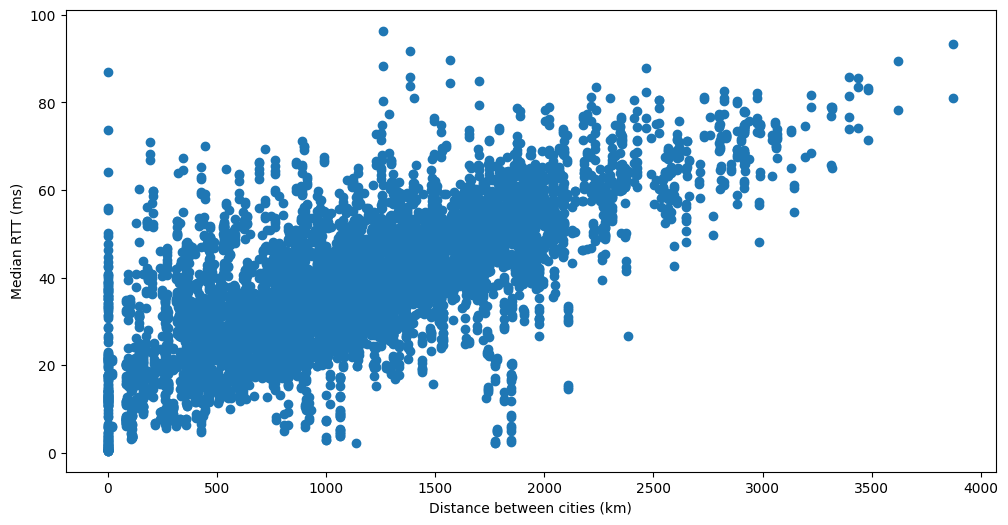
\includegraphics[width=\textwidth]{figures/mechanisms/nw_proximity/shortest-rtt-vs-dist.png}
        \caption{Variation of network RTT with geographical distance between Edge Sites.}
        \label{fig:geodist_vs_rtt}
    \end{subfigure}%
    ~ 
    \begin{subfigure}[t]{0.45\textwidth}
        \centering
        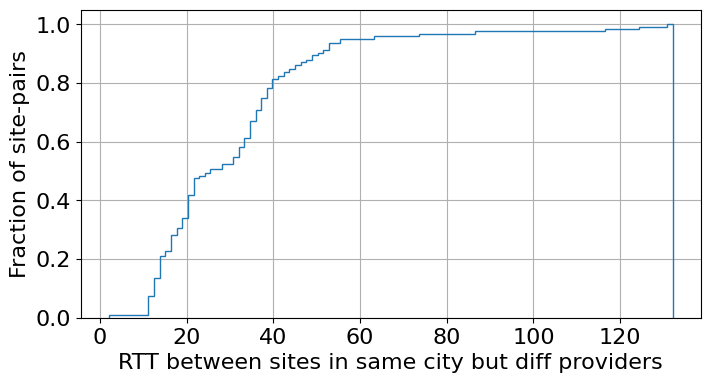
\includegraphics[width=\textwidth]{figures/mechanisms/nw_proximity/same_city_diff_provider_rtts.png}
        \caption{Client-Site RTT for sites selected by transforming the geographical distance into network RTT and uniformly choosing one among the set of sites satisfying the latency constraint.}
        \label{fig:same_city_diff_prov}
    \end{subfigure}
    \caption{Variation of network RTT between edge sites with respect to geographical distance. \todo{Improve visibility of fonts}}
\end{figure*}

\begin{figure*}[t!]
    \centering
    \begin{subfigure}[t]{0.45\textwidth}
        \centering
        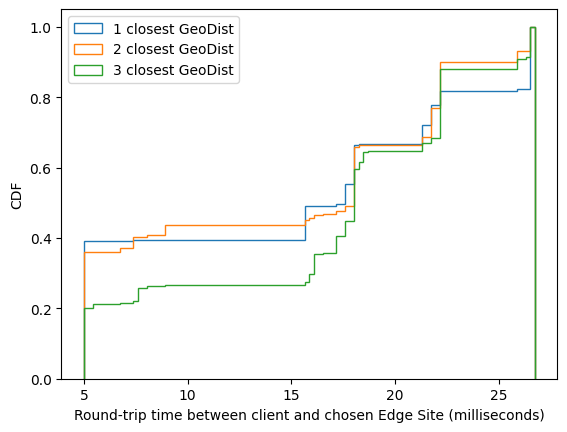
\includegraphics[width=\textwidth]{figures/mechanisms/nw_proximity/geodist_greedy.png}
        \caption{Client-Site RTT for sites selected by Greedy approaches. In the case that the closest site is overloaded, the next closest site is considered and so on.}
        \label{fig:geodist_greedy}
    \end{subfigure}%
    ~ 
    \begin{subfigure}[t]{0.45\textwidth}
        \centering
        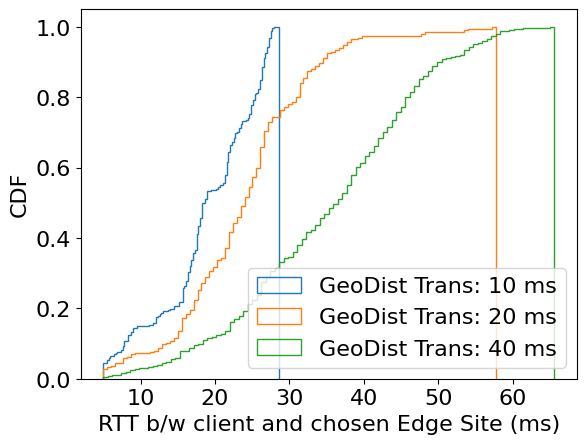
\includegraphics[width=\textwidth]{figures/mechanisms/nw_proximity/geodist_trans_rtt.png}
        \caption{Client-Site RTT for sites selected by transforming the geographical distance into network RTT and uniformly choosing one among the set of sites satisfying the latency constraint.}
        \label{fig:geodist_trans}
    \end{subfigure}
    \label{fig:baseline_proximity_policies}
    \caption{Performance of Edge Site selection approaches that rely on geographical distance as a proxy for network proximity.}
\end{figure*}

\par We evaluate the efficacy of the aforementioned baseline proximity estimation techniques - the greedy distance-minimization approach and the one that transforms geographical distance to network RTT. For this experiment, we consider the infrastructure topology of the city of Shanghai as described in \cref{sec:nep_infra_topology}. We simulate clients at randomly (uniformly) chosen cell tower locations and aim to find an Edge site to host its application instance using one of the above two policies. The goodness of an edge site selection is quantified by the observed RTT between the client and chosen edge site. 
\par The Greedy policy always selects the closest Edge site in terms of geographical distance between the client and the site. In case the chosen Edge site is undergoing compute overload, the policy selects the next closest site, and so on. The other site selection policy that we evaluate is one that transforms the geographical distance between client and edge site to network round-trip time and uses this estimate to filter out those sites that can meet the latency bound imposed by the application. Among the filtered sites, the policy uniformly selects one so as to minimize workload skews.
\par \cref{fig:geodist_greedy} shows the observed RTT when selecting site using the greedy approach. For more than 50 percent of the clients, the geographically closest site is not the one that it is directly connected to over the network, and hence, traffic needs to go through the network provider's core, or through the Internet to get to the selected site. Since there is no correlation between geographical distance and network RTT, this behavior is similar for 2nd and 3rd closest sites as well. For the distance-RTT transformation based approach, we compare the site selection with an application-imposed RTT bound of 10, 20 and 40 milliseconds. We see however, that the transformation does not sufficiently filter out infeasible sites and a large majority of clients have the bound violated.
\par The key takeaway from the above experiments is that using geographical distance between system components overlooks the fundamental aspect of real-world network topologies, in that the network route taken by packets seldom aligns with the geographically shortest path between the source and destination entities. Furthermore, there are additional delays caused at the various intermediate hops. Hence, any proximity estimation technique that aims at estimating network communication latency should derive its information from actual measurement of the network latency between system entities.

\subsection{Interface provided to control-plane}
All system components of the platform service (clients, worker nodes, data nodes, etc.) are assigned a unique network proximity identifier. The network proximity mechanism then provides the platform service a function \textbf{NetworkRTT} which takes as input the IDs of two system components and returns the estimated network round-trip time between the two components. 

\subsection{Using network proximity mechanism for compute/data placement}
\label{sec:policy_using_nw_prox}

We now demonstrate the use of the proposed Network Proximity Estimation mechanism for implementing a control-plane policy, specifically the broker selection policy for a publish-subscribe system (\cref{fig:nw_proximity_pubsub_e2e_latency}). This control-plane policy selects the broker to host a given topic such that the end-to-end message delivery latency for all publisher-subscriber pairs is under the latency threshold for the topic, as shown in \cref{fig:nw_proximity_pubsub_e2e_latency}. As described in \cref{algo:pubsub_nw_prox_example}, it iterates over all the potential brokers and computes the worst-case communication latency if the topic is hosted on each of those brokers. The worst-case communication latency is the sum of the maximum publisher-broker network latency and the maximum broker-subscriber network latency. The sum of worst-case communication latency and processing latency on the broker gives the worst-case end-to-end latency for that topic. All the brokers that have the worst-case end-to-end latency under the topic-specific threshold are selected as candidates. The policy finally selects the candidate currently serving the lowest message rate among all candidates to ensure load balancing among brokers.

\begin{figure}
\centering
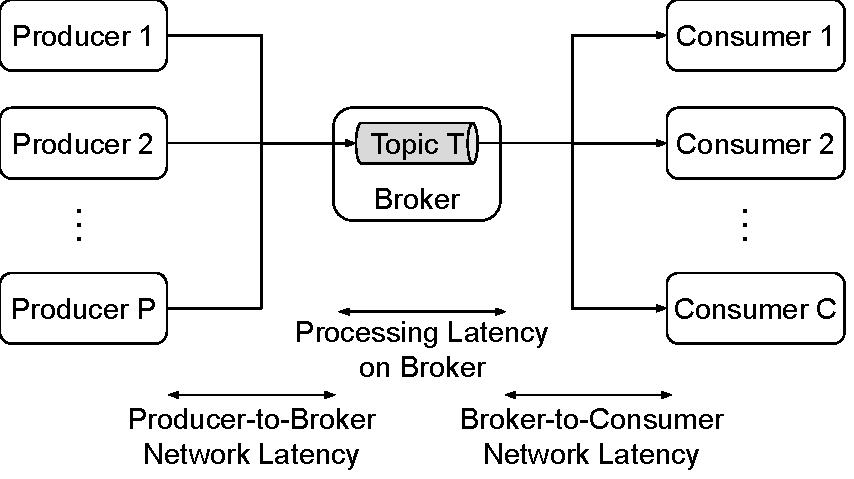
\includegraphics[width=0.6\linewidth]{figures/mechanisms/nw_proximity/pubsub_e2e_latency.pdf}
\label{fig:nw_proximity_pubsub_e2e_latency}
\caption{An instance of publish-subscribe service as an exemplary platform-service that requires information about network communication latency to compute the end-to-end latency experienced by the application. In this example, the end-to-end latency is the message delivery latency from any producer to all consumers for a given topic. The end-to-end latency is given by the sum of the maximum network latency from any producer to the broker, the processing latency on the broker, and the maximum network latency from the broker to any consumer.}
\end{figure}

\begin{algorithm}
\caption{Broker selection policy for topic $T$ with end-to-end latency threshold $L_{th}$}
\label{algo:pubsub_nw_prox_example}
\begin{algorithmic}
\Require topic $T$
\Require latency threshold $L_{th}$
\State $prod \gets \text{ set of producers for }T$
\State $cons \gets \text{ set of consumers for }T$
\State $candidates \gets \{\}$
\For{$\text{each broker } b$} 
    \State $nw\_lat \gets max_{p \in prod} \dfrac{1}{2} \cdot NetworkRTT \left( p, b \right) + max_{c \in cons} \dfrac{1}{2} \cdot NetworkRTT \left( c, b \right)$
    \State $e2e \gets nw\_lat + proc\_latency \left( b \right)$
    \If{$e2e \leq L_{th}$}
        \State $candidates \gets candidates \cup \{b\}$
    \EndIf
\EndFor
\Return broker in $candidates$ with lowest $msg\_rate$
\end{algorithmic}
\end{algorithm}

\section{End-to-End Monitoring Mechanism}
Situation-awareness applications require that the end-to-end latency and spatial affinity requirements are satisfied for the entire lifetime of the application, so that correct functionality can be guaranteed. However, given the constant mobility of end-clients, these requirements are likely to be violated repeatedly and frequently. For instance, a car moving away for the Edge Site currently serving the vehicle-local processing component would incur higher end-to-end processing latency. Similarly, a vehicle that moves out of the geographical area being served by the current region-level application component would receive fused sensor data updates that no longer pertain to its spatial context. Hence, the control-plane of the platform services are required to constantly monitor the running applications for such violations, perform root-cause analysis for determining the cause of the violation, and take appropriate reconfiguration action(s) to resolve the violation. Examples of such a reconfiguration would be the migration of the application component to an Edge Site that is closer (in terms of network proximity) to the end-client to ensure end-to-end latency satisfaction, or the re-mapping of the end-client to an application component that has the same spatial context as the end-client to satisfy the spatial affinity requirement.
\begin{figure}
\centering
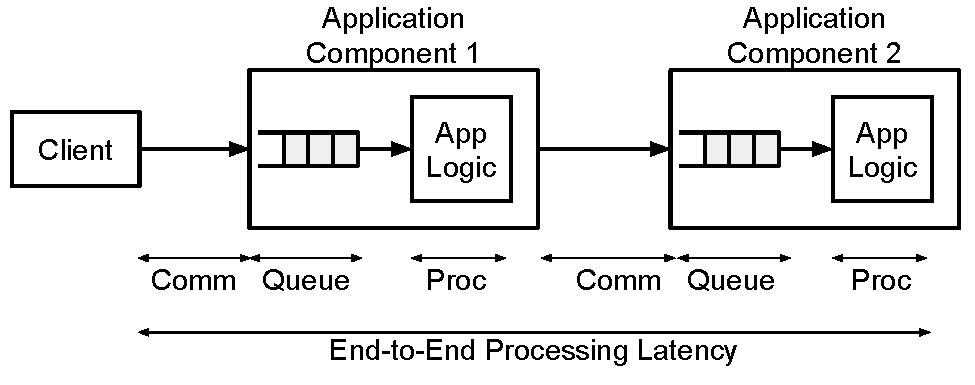
\includegraphics[width=0.75\linewidth]{figures/mechanisms/monitoring/pipeline_latencies}
\caption{A breakdown of the end-to-end processing latency of an application pipeline into its constituent latencies.}
\label{fig:pipeline_latencies}
\end{figure}
\par Thorough monitoring of applications running atop platform services is a non-trivial task because there can be multiple sources of performance violation. For instance, as shown in \cref{fig:pipeline_latencies}, the observed end-to-end latency of the application instance is a sum of the queuing, execution and downstream communication latencies of each operator in the pipeline.  Thus, in order to detect a violation of the end-to-end latency requirement and identify the root-cause requires the monitoring of all the component latency metrics as independent timeseries and their aggregation and analysis. Each platform service has a notion of an \textit{application unit}, which represents an independent set of system entities that do not affect the performance of entities not within the given unit. An example of an application unit is a publish-subscribe topic, which consists of all the producers, consumers and broker hosting that topic. Furthermore, each platform service has its own set of metrics that need to be monitored for each application unit. These metrics then need to be aggregated and analyzed in a platform service-specific way as well to detect violations. The monitoring mechanism needs to scale with an increasing number of application instances being monitored and impose low overhead on the applications and infrastructure.

\subsubsection{Shortcomings of previous work}
\par Application monitoring has been an active area of work in the cloud computing space with a number of research projects and commercial offerings available. In the context of cloud computing, applications typically don't possess end-to-end latency requirements and the goal of monitoring is to ensure that the tail latency of a given service (that could consist of multiple instances) doesn't increase significantly. Platforms such as Prometheus \cite{prometheus} and Monasca \cite{monasca} don't support the aggregation of multiple metrics to study the behavior of end-to-end latency. Furthermore, their architecture is a fully centralized one, resulting in the use of network bandwidth to send the monitoring data to the cloud.
\par Monitoring systems designed for edge computing environments also suffer from limitations, wherein they aggregate measured metrics over geographical regions instead of aggregating multiple metrics pertaining to the same application instance \cite{fmone, gonccalves2021dynamic}. Such systems are not capable of detecting violations of end-to-end performance constraints. Previous contributions to building systems services such as publish-subscribe systems \cite{emma} and distributed application runtimes \cite{foglets} consist of monitoring subsystems that only monitor the the network connectivity between a client and the edge site that it is connected directly to. Since these solutions don't consider end-to-end latency as the primary metric, they would result in triggering more reconfigurations to keep clients connected to the closest edge site than needed.
\begin{figure}
\centering
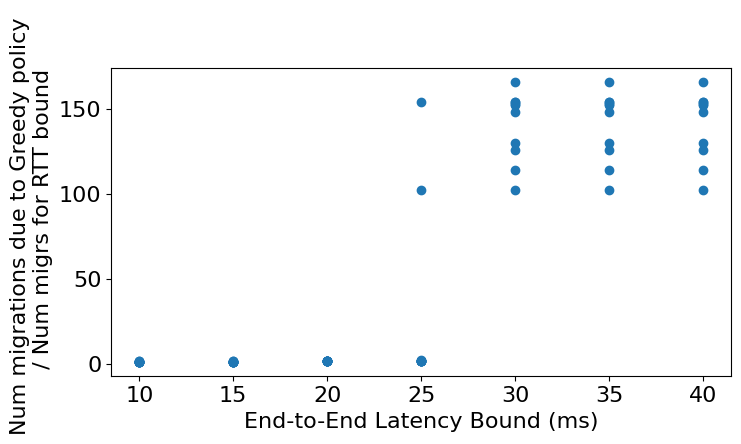
\includegraphics[width=0.75\linewidth]{figures/mechanisms/monitoring/migrations_count.png}
\caption{Ratio of the number of migrations triggered by Greedy monitoring scheme versus those triggered by an optimal policy. The end-to-end latency threshold is varied along the x-axis.}
\label{fig:migration_count}
\end{figure}
\par In the following we show an evaluation of a greedy monitoring approach that aims to minimize the last-mile network latency between the client and the edge-site it directly connects to. The metric of interest is the number of migrations triggered by such a policy compared to an optimal policy that monitors the end-to-end latency and only triggers a migration when the observed end-to-end latency violates the application's threshold. We simulate the mobility of 200 independent clients in the city of Shanghai using the Random Waypoint mobility model and track the number of migrations triggered by both the greedy and optimal policies. In \cref{fig:migration_count}, we present the ratio of the migrations triggered by the greedy policy and that by the optimal policy with increasing end-to-end latency bound. We see that as the end-to-end latency bound increases, the relative number of migrations triggered by greedy policy becomes much higher. This is because, although the greedy policy triggers the same number of migrations as it is independent of the end-to-end latency constraint, the number of migrations triggered by the optimal policy decreases with an increase in the threshold. This necessitates that any useful and efficient monitoring system should consider multiple metrics together that pertain to different components of the end-to-end latency. Violation detection needs to happen for each application-level unit, or application instance, such as a publish-subscribe topic, or one instance of an application pipeline (as shown in \cref{fig:pipeline_latencies}). Hence, metrics that belong to the same application unit should be aggregated together for violation detection and other control-plane policies.

\subsection{Interface provided to control-plane}
The following abstractions are provided to the control-plane of a platform service when using the distributed end-to-end monitoring mechanism.
\begin{itemize}
\item \textbf{RegisterAppUnit.} Registration of an Application Unit when it is created. For instance, when a new topic is created in a publish-subscribe system, the topic should be registered as a new Application Unit. The Monitoring mechanism uses the identifier of the application unit to identify the metrics that pertain to it, and is thus able to perform end-to-end aggregation on them.
\item \textbf{RegisterMetric.} System components can register custom metrics and publish measurements to them. The metrics are annotated with the application unit that they correspond do, as well as custom platform-specific tags. The following snippet shows an example, which measures the network latency of an instance of the pipeline stage shown in \cref{fig:app_pipeline} to its downstream component. In the given platform service, the application unit that a metric belongs to is the downstream-most application component, or the root component. In this example, the application unit is the application component instance $L_0$.
\begin{minted}{yaml}
-   entity_id : "L10"
    entity_type: "APP"
    app_unit: "L0"
    metric: "net_latency"
\end{minted}
Each metric stream is represented an ordered sequence of measurements along with their timestamps as shown in \cref{eq:metric_stream}.
\begin{equation}
M = \left[ \cdots , \left( t, v \right) , \cdots \right] \text{ where } 0 < t < \infty
\label{eq:metric_stream}
\end{equation}

\item \textbf{AlignMetrics.} The control-plane policy can time-align the measurements for a specific metric into well-defined buckets. This interface is necessary as a preprocessing step before multiple metrics can be aggregated together. Since different metrics are likely to be recorded at different instants in time, aligning them in time allows the values from different metrics to be processed together, such that two values from different metrics that were collected at roughly the same time can be processed together. \cref{fig:time_alignment} illustrates the time alignment of a metric for a fixed size time bucket, and all measurements within a given bucket are aggregated by taking an average over them. The platform service is supposed to provide the bucket size $B$ and the aggregation function $func$ for aggregating a metric $M$.
\begin{figure}
\centering
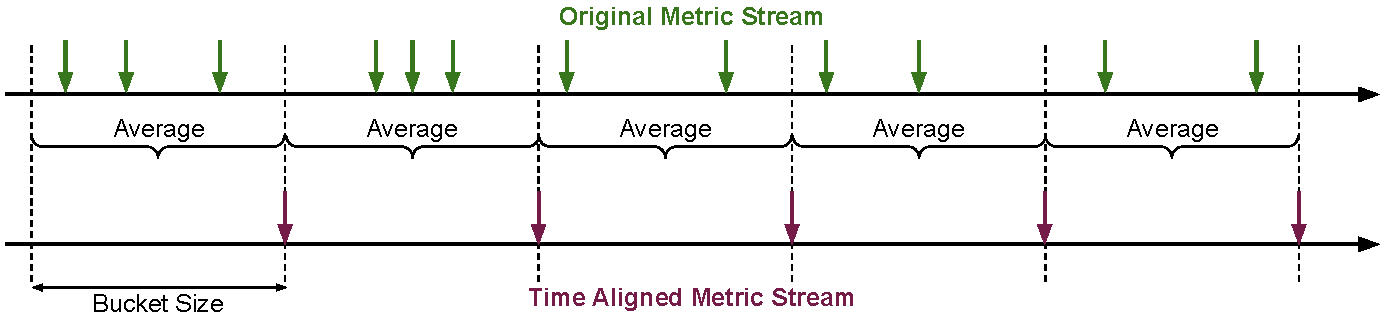
\includegraphics[width=\linewidth]{figures/mechanisms/monitoring/time_alignment}
\caption{Illustration of time alignment of metrics. The individual measurements within each time bucket are aggregated using average function to generate the measurement for that bucket. The time alignment function takes as input a metric stream and time bucket size and returns another stream.}
\label{fig:time_alignment}
\end{figure}
\begin{multline}
ALIGN^{func}_{B} \left( M \right) = \left[ \cdots , \left( t, v \right) , \cdots \right] \text{ where } t = n\cdot B \text{ and } 0 < n < \infty \\ \text{ and } v = func \left( \{ v' : \left( t', v'\right) \in M \text{ and } B\cdot \left( n-1\right) < t' \leq n \cdot B \} \right)
\label{eq:metric_stream}
\end{multline}

%\item Platform-specific definition of the system entity processing all the metrics of a given application unit for performing aggregation and violation detection. For instance, in the case of a publish-subscribe system, all the metrics pertaining to a specific topic can be processed at the broker serving that topic.
\item \textbf{ProcessMetrics. }This interface allows platform-services to specify logic for metrics aggregation and violation detection policies. The logic should be able to query metrics using the aforementioned tags, generate new aggregated metrics, and call an endpoint in the platform service's control-plane to notify it of a violation and provide information about the root cause. The policy should also be able to access certain configurations of the platform service, such as the mapping of child application components to parent application component for the application orchestrator, or the mapping of topics to brokers in the case of publish-subscribe system. Information about such configurations is useful for knowing which metrics need to be aggregated together.
\item \textbf{QueryMetrics. }The logic provided to the end-to-end monitoring mechanism via the ProcessMetrics interface should be able to query metrics using their labels.
\end{itemize}

\subsection{Demonstration of using end-to-end monitoring for control-plane policy of a platform service}
In this section, we show how the end-to-end monitoring mechanism will be used for implementing the control-plane policy for detecting violation of end-to-end processing latency for a geo-distributed application orchestrator system. For this example, we would restrict the discussion to clients and application instances for a single application unit, but the approach generalizes to multiple units.
\begin{enumerate}
\item The library of the platform service running alongside each client and backend application instance generates two metrics - namely the processing latency and network latency to the immediately downstream application component instance (called \textit{parent}). For application component $e$ denote them as $proc_e$ and $net_e$.\\
\begin{minipage}{0.45\textwidth}
\begin{minted}{yaml}
-   entity_id : "L20"
    entity_type: "CLIENT"
    app_unit: "L0"
    metric: "proc_latency"
\end{minted}
\end{minipage}%
\hfill
\begin{minipage}{0.45\textwidth}
\begin{tabular}{p{\textwidth}}
\begin{minted}{yaml}
-   entity_id : "L10"
    entity_type: "APP"
    app_unit: "L0"
    metric: "net_latency"
\end{minted}
\end{tabular}
\end{minipage}

The above listings show definitions of metrics corresponding to the processing and network latency of the application component instance $L_{20}$ and $L_{10}$ respectively in the application instance shown in \cref{fig:app_pipeline}. Both these component instances pertain to the application unit which is associated with the "root" application component instance $L_0$. 
\item The platform service requests for time-alignment of all the metric streams using the function $ALIGN^{AVG}_{5secs}$. We denote the aligned version of metric stream $M$ as $M*$.
\item The control-plane policy for detecting violations of end-to-end processing latency performs calculations for each of the root application instances, which we denote as $L_0$. It selects the latency metrics corresponding to the clients that are connected to $L_0$ as shown in \cref{fig:app_pipeline}. It uses a query like the following to select the latency metrics for all the clients that are connected to the root application component $L_0$.
\begin{minted}{sql}
SELECT METRICS WITH entity_type="CLIENT" AND app_unit="L0"
\end{minted}
\begin{figure}
\centering
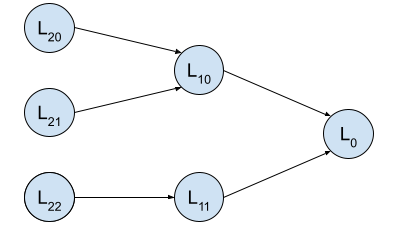
\includegraphics[width=0.5\textwidth]{figures/mechanisms/monitoring/app_pipeline.png}
\caption{Schematic of a typical situation-awareness application. The application model resembles a tree, with the leaf vertices corresponding to clients. Each vertex has a parent vertex except the root vertex.}
\label{fig:app_pipeline}
\end{figure}
\item The above set of metrics are then grouped by the field $entity\_ID$ because they contain both processing latency and network latency metrics for each client. Grouping them by $entity\_ID$ allows the policy to separate the metrics of a specific client from other clients.
\item For each client component $c$, the policy computes the set of application components $S_c$ that process data generated by $c$. The following pseudocode illustrates this computation.
\begin{algorithmic}
\State $n \gets c$
\State $S_c \gets \{\}$
\While{$n \neq \phi$} 
    \State $S_c \gets S_c \cup \{ n \}$
    \State $n \gets M \left[ n \right]$
\EndWhile
\end{algorithmic}
We use the notation $M \left[ n \right]$ to denote the downstream application component reading the output of $n$. The downstream application component for the root component $L_0$ is designated to be null ($\phi$). This information is obtained from the application orchestrator platform service's control-plane metadata about application mapping.

\item For each client $c$, now it is possible to compute a time-aligned metric stream which records the end-to-end processing latency for $c$.
\begin{equation}
E2E_c^* = \sum_{e \in S_c} proc_e^* + net_e^*
\end{equation}
For those clients whose end-to-end latency estimation exceeds the application's threshold, a reconfiguration action is triggered. The objective of the reconfiguration action is determined by root-cause analysis, wherein the relative contribution of each of the component latencies toward the violation end-to-end latency violation is analyzed. In case the violation is most significantly caused by an increase in communication latency between an upstream-downstream application component pair $\left( l1, l2 \right)$ then $l1$ is re-mapped to another downstream component instance that has a better network latency. Similarly, if the root-cause is an increase in processing latency at a certain component instance $l$, then it is either allocated more resources to bring down the processing latency. If resource allocation cannot be increased due to capacity constraints, a fraction of its immediately upstream component instances are mapped to another instance so as to reduce the workload on $l$.
\end{enumerate}


    %\chapter{Design Space Exploration for Implementation of Proposed Mechanisms}
\label{sec:design_space_exploration}

In this chapter, we consider multiple design choices for implementing the mechanisms proposed in this dissertation. The aim of the design space exploration is to come up with the best design for each mechanism in the context of operation in a geo-distributed setting. The chosen design should be scalable with respect to the number of clients and Edge sites, should perform the desired functionality expected from the mechanism effectively and not consume high resource overhead on the scarce Edge resources.

\section{Dynamic Spatial Context Management}

We divide the design space exploration of the dynamic spatial context management mechanism into two parts. We first explore the appropriate choice of the spatial partitioning technique, that divides a geographical space into multiple tiles, and assigns spatial context to clients, application components and data-items. The second exploration we carry out is the system architecture for continuously monitoring client location and triggering a migration to a new tile when the client enters the new tile. We define the requirements expected from both these components of the architecture, enumerate the metrics of interest and carry out evaluations to quantify the performance of candidate design choices. Based on the results of the evaluations, we choose the design choice that performs best to build the dynamic spatial context management mechanism.

\subsection{Client Workload assumed}
The behavior of spatial context management is dependent on the locations of clients within the geographical space in question. We assume that an application would define a large geographical area (typically the size of a city) wherein its clients would be located, and the spatial context of a client would be a subset of the entire geographical area. For this design space exploration, we consider the area of downtown Shanghai where clients are spawned at random locations following a uniform probability distribution. We generate trajectories of 1000 clients that move in the geographical space following the random waypoint mobility model. 

\subsection{Maintaining Spatial Partitioning}
The objective of a spatial partitioning technique in the context of the dynamic spatial context management mechanism is to be able to associate multiple clients that belong to the same spatial context together. Each of the regions (that we call \textit{tiles}) created out of spatial partitioning could be mapped to an application instance, in which case each application instance would serve the clients that belong to that tile. In another scenario, the spatial partitioning could serve as a range query lookup tool for spatially distributed data, and a tile could form the unit of data-sharing. We denote the number of entities (clients or data-items) mapped to a tile as the \textit{occupancy} of that tile. In both these scenarios, a tile which has a very high occupancy would result in compute overload at the associated application instance or high range-query overhead for the mapped data-items. Hence, the requirement is that the occupancy of each tile should be low enough so as to not cause performance degradation due to overload. 
\subsubsection{Metrics of Interest}
Considering a static scenario, with no mobility of clients, as an example, a trivial mapping that uses a very fine-grained spatial partitioning to map each entity to a distinct tile would result in the occupancy of each tile being minimal, because each tile would be associated with either exactly 0 or exactly 1 entity. However, this would also result in the existence of a large number of tiles, which is unnecessary and even counter-productive, because, for instance, applications do require that multiple clients be mapped to the same tile so that inter-client coordination can be possible. Furthermore, continuous client mobility would trigger very frequent requests for re-mapping clients to different tiles. Hence, we identify two metrics for quantifying the \textit{goodness} of a spatial partitioning scheme. 
\begin{itemize}
\item \textbf{Maximum Tile Occupancy.} We measure the maximum occupancy at any tile at any point of time, which would quantify the workload experienced by the associated application component or data-storage node. 
\item \textbf{Number of Active Tiles}. We measure the number of tiles being used at any given point of time, i.e., those tiles to which at least one entity has been mapped. Ideally, this number should be as low as possible, so that we don't have a large number of application instances or data nodes, which consume resources on the Edge.
\end{itemize}
\par For this evaluation, we are interested in evaluating spatial partitioning techniques using the aforementioned metrics, while assuming that the spatial context management mechanism had accurate and real-time information about the location of each client. Following the Random Waypoint Mobility model as described earlier, the location of each client is updated every millisecond. The updated locations are fed to the spatial partitioning unit, which updates the client-to-tile mapping. At every time instant we calculate the two metrics of interest, hence generating a time-series for each of the spatial partitioning configurations evaluated. We later average these measurements across time and present a scalar value that represents the performance of the given spatial partitioning technique.

\subsubsection{Candidate Design Choices Evaluated}
We evaluate two spatial partitioning techniques that are common in the literature \cite{mmog_kdtree, talkycars}.

\begin{figure}
\centering
\begin{subfigure}{0.33\textwidth}
  \centering
  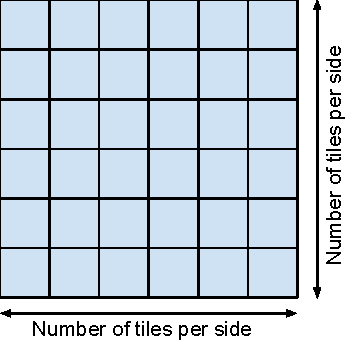
\includegraphics[width=\linewidth]{figures/design_space/spatial/static_partitioning.pdf}
  \caption{Illustration of partitioning geographical space using the static partitioning technique.}
  \label{fig:static_part}
\end{subfigure}%
~~~~~~~~
\begin{subfigure}{0.66\textwidth}
  \centering
  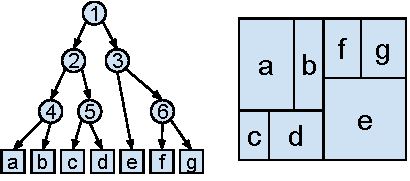
\includegraphics[width=\linewidth]{figures/design_space/spatial/kdtree_partitioning.pdf}
  \caption{Illustration of partitioning geographical space using the KD-Tree technique.}
  \label{fig:kdtree_part}
\end{subfigure}\par\medskip
\caption{Illustration of the candidate spatial partitioning approaches evaluated in the design space exploration. In both the figures, the rectangular area represents the application's geographical coverage and each rectangle inside it represents a tile to which entities are mapped.}
\end{figure}

\begin{itemize}
\item \textbf{Static Partitioning}. Similar to GeoHash, this geo-indexing technique statically divides the  geographical space into a number of tiles. Since we are not interested in the numeric value of the tile's identifier (unlike typical use-cases of geo-indexing approaches such as GeoHash), we simplify the partitioning by assuming that geographical space is partitioned into a grid of squares, and the side length of each square is configurable. Each tile can then be represented by a tuple $\left( row, col \right)$, where $row$ and $col$ represent the position of the tile in the grid. Given the location of a client, it is straightforward to map it to a tile based on the size of each tile and the size of the total geographical area.
\item \textbf{KD-Tree based Partitioning} uses a two-dimensional KD-tree to partition geographical space. The vertices in the KD-tree represent geographical areas, with the root vertex representing the entire geographical space in question, while the leaf vertices represent the tiles. The spatial bounds of a vertex are fixed and decided when creating the vertex. Looking up the tile that a given client belongs to requires performing a traversal starting from the root vertex down to the leaf vertex that represents the actual tile. At each step in this traversal, the bounds of the child nodes and the given client's location are used to decide which of the child nodes to move to next. The size of each tile is not fixed, rather it changes dynamically as the tree is updated. The only constraint that is enforced by the tree is that the number of clients mapped to a specific tile should not exceed an \textit{occupancy threshold}. If the occupancy of a particular tile becomes higher than the threshold, the tile is split and two children tiles are created. Furthermore, if the total occupancy of two tiles that have the same parent tile is less than the occupancy threshold, the two child tiles are merged.
\end{itemize}

\begin{figure}
\centering
\begin{subfigure}{0.45\textwidth}
  \centering
  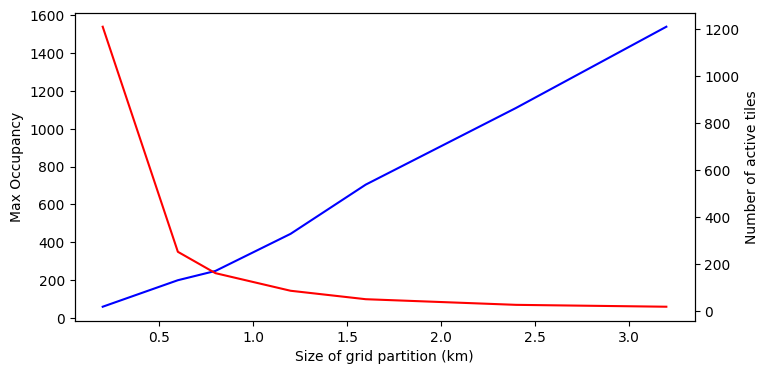
\includegraphics[width=\linewidth]{figures/design_space/spatial/metrics_Grid.png}
  \caption{Variation of metrics of interest for the static partitioning technique with changing number of tiles along each side of the geographical space.}
  \label{fig:static_part}
\end{subfigure}
~~~~
\begin{subfigure}{0.45\textwidth}
  \centering
  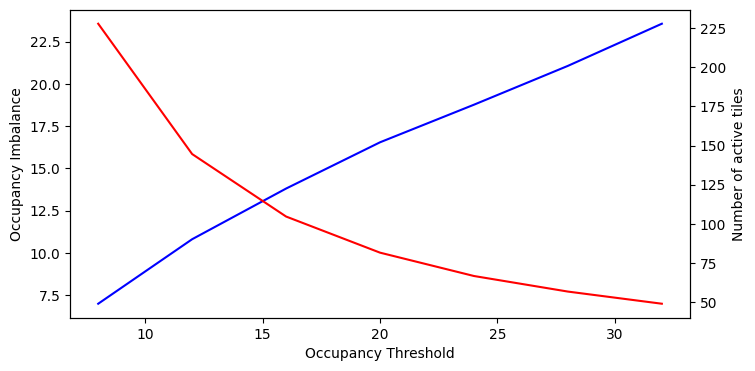
\includegraphics[width=\linewidth]{figures/design_space/spatial/metrics_KDTree.png}
  \caption{Variation of metrics of interest for the KD-Tree based dynamic spatial partitioning technique with changing occupancy threshold per tile.}
  \label{fig:kdtree_part}
\end{subfigure}\par\medskip
\end{figure}

We first evaluate the performance of the Static Partitioning technique against the aforementioned client workload. We evaluate the two metrics of interest - namely Maximum Occupancy and Number of active tiles. The evaluation is done with several different configurations of each partitioning technique. \cref{fig:static_part} shows the variation of the Maximum occupancy and the Number of active tiles as a function of the side-length of each geographical partition. As the size of the grid partition increases, the maximum occupancy grows, along with a decrease in the number of active tiles. This tradeoff is shown in \cref{fig:spatial_tradeoff} as well.
\par Next we perform the same experiment with the KD-Tree based spatial partitioning technique, wherein we configure the Occupancy Threshold for a tile. We vary the occupancy threshold from 8 to 32 and plot the metrics of interest in \cref{fig:kdtree_part}. The metrics show a similar behavior as in \cref{fig:static_part}. As the occupancy threshold increases, the number of tiles that exist in the system decreases, because each tile can hold more clients. This also results in higher maximum occupancy in the system.

\begin{figure}
\centering
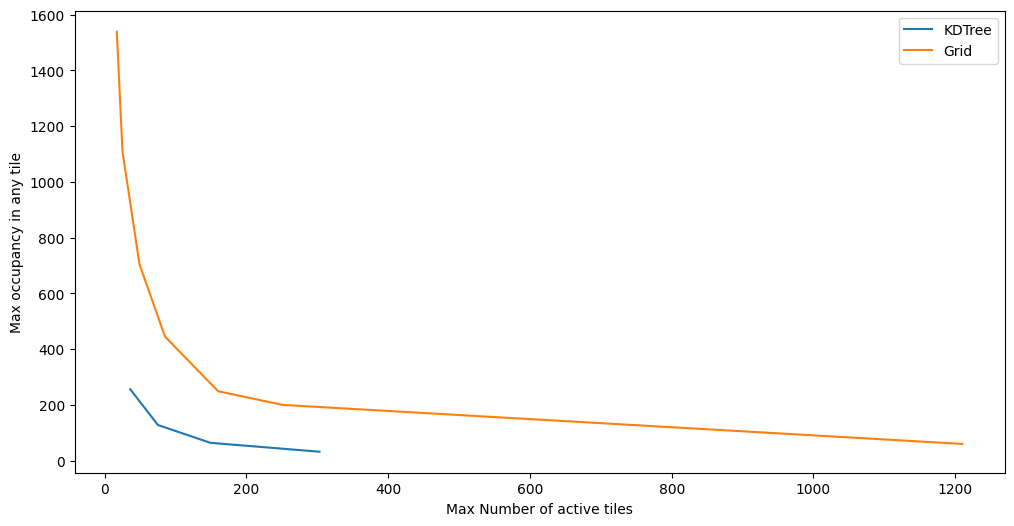
\includegraphics[width=0.75\linewidth]{figures/design_space/spatial/spatial_partitioning_tradeoff.png}
\caption{Tradeoff between the the two metrics of interest - Maximum Occupancy and Number of active Tiles - for the two types of partitioning techniques evaluated. We changed the configuration of each partitioning technique and repeated the experiment to obtain a range of performance output, which shows the tradeoff between the two metrics.}
\label{fig:spatial_tradeoff}
\end{figure}

\cref{fig:spatial_tradeoff} shows the tradeoff between the two metrics of interest for the two spatial partitioning techniques that we evaluate. Both the partitioning techniques show similar behavior for the tradeoff curve, where an increase in Maximum Occupancy results in a decrease in the number of active tiles, and vice versa. However, the absolute values of both the metrics are much lower for the KD-Tree based partitioning than the Static partitioning. This is because the KD-Tree partitioning builds tiles based on the physical distribution of clients, instead of being predefined in the case of Static partitioning. Because of this adaptive partitioning that KD-Tree allows, a smaller number of tiles are able to uniformly divide the clients. Hence, we choose KD-Tree based dynamic spatial partitioning technique for building the dynamic spatial context mechanism.
\subsection{Monitoring Client Location}
Monitoring the current location of clients is necessary for maintaining the KD-Tree based spatial partitioning because of two main reasons - (i) it provides the information necessary for maintaining the occupancy information, and trigger the remapping of a client to another tile when it leaves the current one, and (ii) when partitioning a tile, updated client locations provide hints about how to partition the tile so that a roughly equal number of clients are present in both the children tiles.
The spatial partitioning is maintained in a centralized location so that an authoritative copy can be maintained. Sending location updates from all clients to the centralized location consumes network bandwidth as well as creates a large number of occupancy updates which don't necessarily result in a change in the current tile. 
\subsubsection{Metrics of Interest}
We choose two metrics of interest for evaluating the candidate designs for location monitoring module of the dynamic spatial context management mechanism. 
\begin{itemize}
\item \textbf{Messaging Overhead. } We measure the number of location monitoring messages that need to be sent to the centralized location. This metric should be minimized to improve system scalability. 
\item \textbf{Total Occupancy Violation Time. } We measure the sum of all the time durations for which some tile's occupancy threshold was violated. Since the occupancy threshold is set by the application, violating it would result in suboptimal performance.
\end{itemize}

\subsubsection{Candidate Approaches Evaluated}
\begin{itemize}
\item \textbf{Centralized Approach. }A straightforward design for maintaining updated client locations is to send all location updates from clients to the centralized location holding the authoritative copy of the spatial partitioning. Clients receive the identifier of the current tile based on their current location, and if the received tile identifier is different from the current tile, they would connect to the application instance corresponding to the new tile. The centralized spatial partitioning unit would transparently handle scenarios when the partitioning is updated due to tile merging or splitting operations. Although this approach is very straightforward to design and implement, it suffers from high overhead of constantly monitoring the locations of all clients at all times.
\item \textbf{Distributed Approach. } Unlike the centralized approach, where the client simply reports the current location to the spatial partitioning module and receives the identifier of the current tile, the distributed approach maintains a cache of the spatial partitioning locally. The local cache is invalidated and updated every time the authoritative copy at the centralized location is updated due to tile merging or splitting operations. The cache is then used by the client to keep track of its location with respect to the current tile, and in the event that its location leaves the current tile, it triggers a migration to connect to the new tile. The cache also periodically report its location to the authoritative copy so that tile split operations can effectively partition clients into the child tiles equally. The periodicity of reporting location to the control-plane is configurable.
\end{itemize}

\begin{figure}
\centering
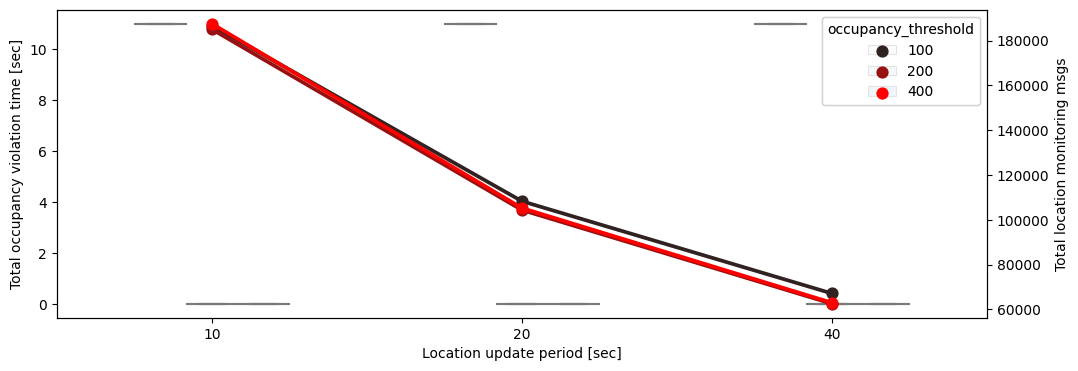
\includegraphics[width=\linewidth]{figures/design_space/spatial/loc_update_period_tradeoff.png}
\caption{Effect of location update period on the duration of occupancy violation faced by tiles and the amount of location monitoring messages needed to be sent to the control-plane.}
\label{fig:location_update_period}
\end{figure}
\cref{fig:location_update_period} shows the variation of duration of occupancy violation and location monitoring messages with increasing location update period. The increase in location update period does not have any noticeable impact on the violation duration, however it results in a significant drop in the number of messages for monitoring location of clients. Since the client immediately sends a location update when it leaves the current tile irrespective of the location update period, the violation duration is not dependent on location update period. In fact, for occupancy threshold of  200, the violation duration is 0, which shows that there are no occupancy violations. Hence, choosing a high location update period does not significantly impact the total violation duration, but heavily reduces location monitoring traffic.

\section{Network Proximity Estimation}

Control-plane policies of platform services need to make data and compute placement decisions so as to satisfy data processing latency constraints. In an Edge setting, network communication latency forms a significant portion of the end-to-end latency. Previous work in the cloud computing domain has come up with accurate techniques for estimating computation latency, but didn't consider communication latency due to the rather homogeneous and well connected nature of datacenter network topology. In an Edge infrastructure, it is important to be able to accurately estimate the network latency between a pair of system entities, so that the control-plane policy can make a data/compute placement decision to satisfy end-to-end latency.
\par The network proximity estimation cannot be done using active measurements at the time of execution of the control-plane policy logic, because a typical policy evaluates several candidate nodes (e.g., to select best application placement candidate) and therefore  requires pairwise network latency between several pairs of nodes to make its decision. Waiting for the measurements to complete in the critical path of policy execution would severely impact the responsiveness of the control plane. Hence, the network proximity estimation mechanism needs to continuously maintain network proximity metadata for each node in the infrastructure. The size of the metadata needs to be tractable so that it can be efficiently queried to estimate pairwise network latency.
\par The mechanism should estimate pair-wise network latency with high accuracy. Furthermore, it should be able to quickly adapt to changes in network topology due to client mobility or link failures. Both the accuracy and recovery-time of the mechanism to topology dynamism should not deteriorate with increasing number of nodes, meaning that the mechanism should be scalable.

\subsection{Metrics of Interest}
We consider the following metrics of interest when evaluating the candidate design choices for network proximity estimation mechanism.

\begin{itemize}
\item \textbf{Latency Estimation Error.} We measure the root-mean squared error between the estimated and the actual (ground-truth) network latency. For a pair of nodes $i$ and $j$, the estimated and actual network latencies for the pair $\left( i, j\right)$ is denoted by $N_{\left( i, j\right)}$ and $\hat{N}_{\left( i, j\right)}$ respectively. The root-mean squared error in latency estimation is then calculated as shown in \cref{eq:rmsre}.
\begin{equation}
\label{eq:rmsre}
RMSE = \sqrt{\sum_{\forall \left(i, j \right) i \neq j}{\left(N_{\left( i, j\right)} - \hat{N}_{\left( i, j\right)}\right)^2}}
\end{equation}
\item \textbf{Number of Messages Exchanged}. We measure the number of messages exchanged between the various nodes in the system before the error in latency estimation drops below the maximum threshold.
\item \textbf{Amount of Metadata} needed by control-plane policies. We analytically calculate the amount of information that would need to be stored at the control-plane in order to support a typical compute/data placement control-plane policy.
%\item \textbf{Response-Time to Topology Dynamism.} We measure the amount of time taken after a change in a particular node's connectivity before all the nodes are aware of that change. This measures the response-time of the mechanism to react to topology changes.
\end{itemize}

\subsection{Candidate Design Choices Evaluated}
\begin{figure}
\centering
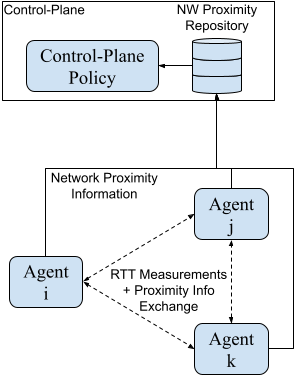
\includegraphics[width=0.4\linewidth]{figures/design_space/nw_prox/basic_sys_arch.png}
\caption{Basic components in the system architecture of the network proximity estimation mechanism. Multiple participating agents communicate among each other to perform actual RTT measurements and compute network proximity, and share the proximity information to one another. The network proximity information is uploaded to a repository in the control-plane from where this information is supplied to control-plane policies.}
\label{fig:nw_prox_arch}
\end{figure}
\cref{fig:nw_prox_arch} shows the basic architecture that the various design choices of the network proximity estimation mechanism have. It is composed of a number of \textit{agents}, with one agent co-located with every system entity with which network proximity needs to be measured. Each agent computes its network proximity to the other agents, and communicates the proximity information to a central repository, which is queried by control-plane policies for estimating network round-trip time (RTT) between any two system entities. The design choices which we explore in this section follow the agent-based architecture, and deal with the kind of communication protocol that each agent follows and the kind of metadata stored by the mechanism that allows it to answer network proximity queries made by control-plane policies. We evaluate the following design choices for the network proximity estimation mechanism. 
\subsubsection{Pair-wise Measurements based Approach}
Representation of network proximity is in the form of a 2-dimensional array $A$, where $A [ i, j ]$ represents the network latency between agent $i$ and $j$. Each participating agent periodically performs a network round-trip time (RTT) measurement between itself and another agent. Each agent uses a round-robin policy to select which other agent it is going to probe to measure the RTT. After each measurement, the agent provides the RTT information between itself and the other agent with which the measurement was performed to the centralized repository of network proximity.

\subsubsection{Network Coordinates}
Network coordinate (NC) systems are distributed protocols to scalably determine the network proximity between a pair of nodes in a distributed system without performing direct measurements \cite{donnet2010survey} between all pairs of nodes. Such systems embed nodes in a geometric space such that the network latency between any two nodes can be estimated by calculating the Euclidean distance between their positions (coordinates) in this space. Previous work on analysis of latencies in the Internet has shown that nodes can be embedded in a 3-dimensional or higher space with relatively high accuracy of network proximity estimation \cite{lee2009suitability}.
\par \noindent \textbf{Embedding in $d$-dimensional space. } Each agent $i$ maintains a network coordinate $x_i$ which is an $d$-dimensional vector. Each agent $i$ periodically performs an RTT measurement with another agent $j$ and also fetches the current network coordinate of agent $j$, which we denote as $x_j$. By using the measured actual RTT $rtt_{i,j}$ between itself and the other agent $j$, the given agent $i$ updates its own network coordinate so as to reduce the error of latency estimation. To do so, agent $i$ first calculates the error in latency estimation, as shown in \cref{eq:rtt_err}.
\begin{equation}
e = rtt_{i,j} - || x_i - x_j ||
\label{eq:rtt_err}
\end{equation}
Each iteration of this coordinate update process at agent $i$ aims at applying a force on $x_i$ so as to move it toward its correct position in the $d$-dimensional space. In other words, if the error calculated in \cref{eq:rtt_err} is positive, $x_i$ would be pushed away from $x_j$, otherwise it will be pulled closer to $x_j$. This notion is captured in \cref{eq:nc_force}, which computes the unit vector of the force to be applied to $x_i$.
\begin{equation}
dir = u \left( x_i - x_j \right) 
\label{eq:nc_force}
\end{equation}
The force that needs to be applied to coordinate $x_i$ is in the direction of the unit vector in \cref{eq:nc_force} and has the magnitude proportional to the error in \cref{eq:rtt_err}. $x_i$ is then updated in the direction of the force by a small and configurable amount.
\begin{equation}
x_i = x_i + \delta \cdot e \cdot dir 
\label{eq:nc_update}
\end{equation}

\par \noindent \textbf{Capturing Access Link Delays. } A number of hosts connected to the Internet today do so behind access links. While the $d$-dimensional Euclidean space is good at modeling latencies in the Internet core, incorporating a scalar $height$ component in the network coordinate significantly improves the network RTT estimation error \cite{vivaldi}. The height component represents the network latency incurred to traverse the access link beyond which latencies can be estimated using the Euclidean coordinate system. The estimated RTT between two agents $i$ and $j$ with combined network coordinates $\left( x_i, height_i \right)$ and $\left( x_j, height_j \right)$ respectively is given by $|| x_i - x_j || + height_i + height_j$. This equation captures the fact that for packets to travel from agent $i$ to $j$, they first have to traverse the access link of agent $i$, travel through the Internet core toward agent $j$ (which can be modeled using Euclidean distance), and then traverse the access link of agent $j$. 

\par \noindent \textbf{Reducing Errors due to Triangle Inequality Violations. } Internet topologies frequently violate the triangle inequality which should ideally hold in a Euclidean space. The triangle inequality requires that the sum of the RTT between agents $i$ and $j$ and that between agents $j$ and $k$ should be greater than the RTT between agents $i$ and $k$. This is violated in real-world network topologies because of heterogeneous routing policies \cite{zheng2005internet}. However, Lee et al. \cite{lee2009suitability} found that such violations occur more frequently  among nodes that are at closer network distances from one another. Hence, they introduce a scalar $adjustment$ term in the network coordinate to account for the non-Euclidean effect due to triangle-inequality violations. The adjustment term is calculated as shown in \cref{eq:adjustment}, where $n$ represents the number of measurements taken.
\begin{equation}
adj_i = \dfrac{1}{2} \cdot \dfrac{\sum_{j} rtt_{i,j} - || x_i - x_j ||}{n}
\label{eq:adjustment}
\end{equation}

\par We employ a popular decentralized network coordinate protocol, Vivaldi \cite{vivaldi} with some enhancements proposed by Ledlie, et al.~\cite{ledlie2007network} and Lee, et al.~\cite{lee2009suitability}. Prior art has shown that NC protocols provide efficient, accurate, and stable latency estimates in the wild~\cite{ledlie2007network}.

\subsection{Evaluations of Candidate Design Choices} 
We evaluate the performance of the candidate design choices for implementing the network proximity estimation mechanism and present the results in this section.

\subsubsection{Accuracy of Network RTT Estimation}
\label{sec:nw_rtt_error}
The network proximity estimation mechanism is expected to accurately estimate network RTT between agents in a real-world geo-distributed infrastructure topology. We use the topology of Edge sites belonging to Alibaba Edge Node Service \cite{xu2021cloud}, which has sites deployed all across mainland China. The dataset provides city-level location of Edge sites along with the actual network RTT between them. In this experiment, in addition to evaluating the error of RTT estimation, we also intend to study how the scale of the infrastructure topology affects the error. We build infrastructure topologies of increasing scale by selecting the top-k cities with the most edge sites and only considering the sites in those cities. Each site runs an agent of the network proximity mechanism, and communicates with potentially every other Edge site to collect RTT and update its network proximity model.
\par \cref{fig:nw_coord_error} shows the evolution of the error in RTT estimation over time for network topologies of increasing scale. The root-mean squared error of latency estimation does increase with an increase in the scale of the network topology, but it converges at around 4.5ms in RTT estimation, which is a reasonable error rate given the variance in ground-truth latency measurements. We don't evaluate accuracy of the pairwise measurements based approach, because the RTT estimates are simply an aggregation of the previously measured RTT values, and hence it would always result in very high accuracy. \begin{figure}
\centering
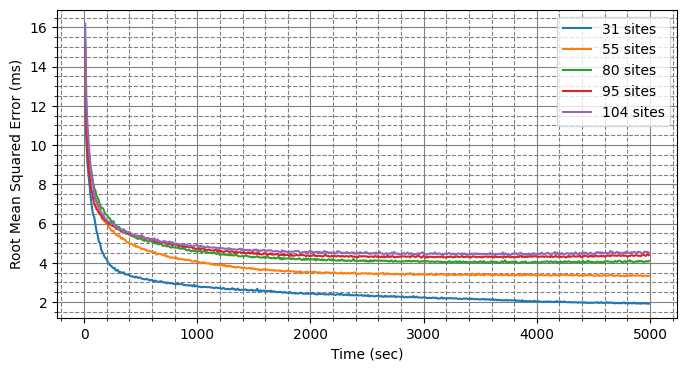
\includegraphics[width=0.75\linewidth]{figures/design_space/nw_prox/error.png}
\caption{Evolution of error in RTT estimation for the network coordinate-based design. The figure shows the RTT estimation error for network topologies of increasing scale.}
\label{fig:nw_coord_error}
\end{figure}

\subsubsection{Communication Overhead}
We now evaluate the amount of communication that needs to happen between the agents of the network proximity estimation mechanism in order to build a reasonably accurate inter-agent network RTT estimation model. We compare the number of messages that need to be communicated between the agents for both the pairwise measurement and network coordinate based designs of the mechanism. 
\par For this experiment, we intend to evaluate network topologies of much larger scale than the Alibaba Edge Node Service topology used in \cref{sec:nw_rtt_error}. We adopt a hub-and-spoke model for generating a synthetic topology for this experiment, with each spoke having a network latency uniformly sampled between 10 and 60 ms. We choose such a model for building the topology because it offers a simple way to model random network characteristics between different pairs of nodes. Each node in the topology runs an agent of the network proximity estimation mechanism. The number of nodes in the topology is varied to evaluate the design choices at different scales.
\begin{figure}
\centering
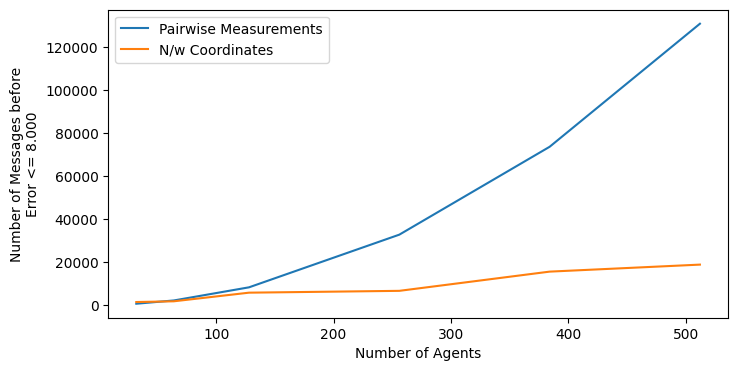
\includegraphics[width=0.75\linewidth]{figures/design_space/nw_prox/comm_overhead.png}
\caption{Communication overhead of the two design choices for network proximity estimation mechanism. The pairwise measurement based design requires $O \left( n^2 \right)$ communication rounds, whereas the network coordinates based approach scales almost linearly.}
\label{fig:comm_overhead}
\end{figure}

\par \cref{fig:comm_overhead} shows the number of communication rounds that need to take place (over all nodes combined) before the network proximity estimation mechanism's error falls below a threshold. The pairwise measurement approach needs to measure the network latency between all pairs of nodes, meaning that it requires $N \left( N - 1 \right)$ rounds of communications, which grows quadratically with increasing number of nodes. On the other hand, the network coordinates approach grows almost linearly, because it only tries to embed nodes in a high-dimensional space based on a small set of measurements. Hence, the network coordinates based approach is a more scalable design for network proximity estimation.

\subsubsection{Size of Network Proximity Repository}
Control-plane policies would frequently query the centralized repository of network proximity estimation to obtain the RTT between a pair of agents. A large metadata would mean that the query would take longer to execute, hence, reducing the speed of control-plane policy execution. We compare the amount of metadata to be stored for the two design choices. 

\begin{figure}
\centering
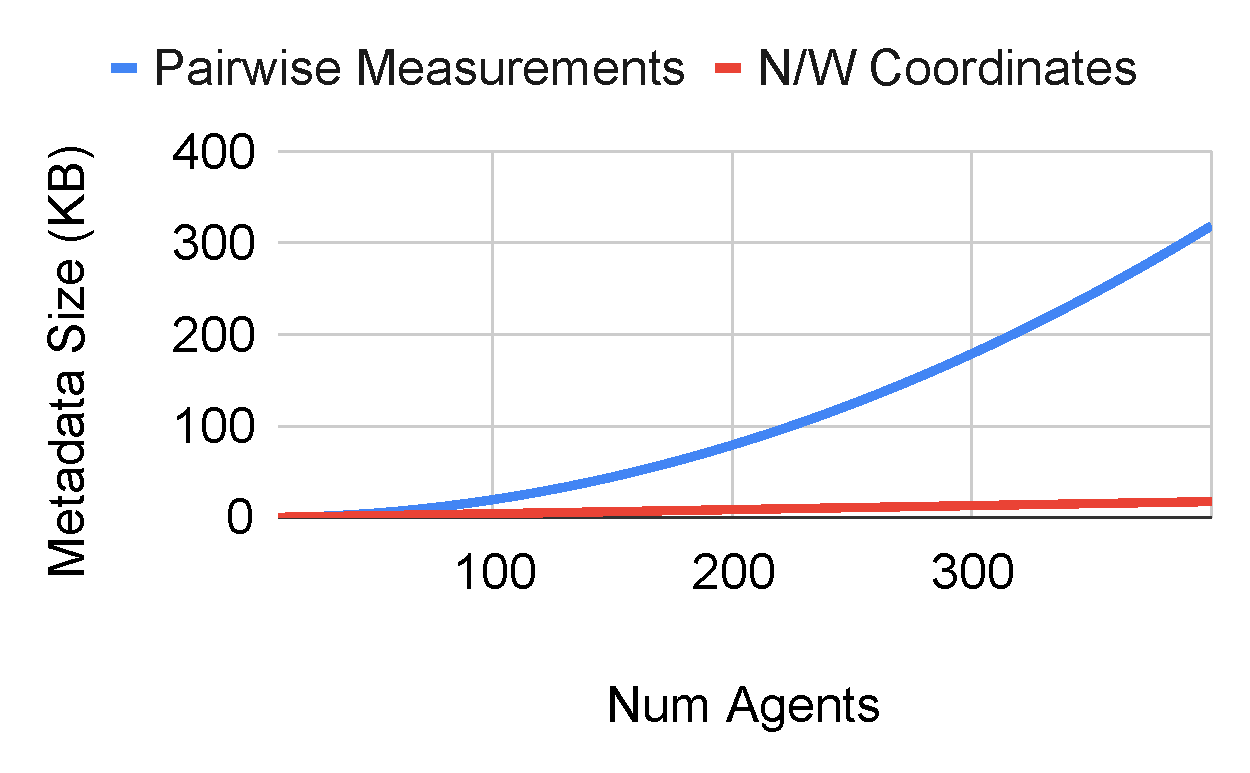
\includegraphics[width=0.75\linewidth]{figures/design_space/nw_prox/metadata_size.pdf}
\caption{Comparison of the size of network-proximity metadata that needs to be stored at the control-plane.}
\label{fig:metadata_size}
\end{figure}

\par \cref{fig:metadata_size} shows how the metadata size grows with increasing number of agents. Since the pairwise measurements based design would need to store the network latency for each pair, the size of the metadata grows quadratically. However, the metadata for the network coordinates based approach consists of one coordinate per agent, which amounts to 44 bytes and grows linearly.

\subsection{Running Network Coordinate Agents on Mobile Clients}
Client mobility results in the change of network routing between client and the Edge infrastructure, since the network access point to which the client is connected changes. This results in a change in network latencies to reach the Edge sites, which affects the ground-truth on which the network coordinates protocol relies for converging to stable coordinates. The end result of these perturbations is a deterioration of the RMSE of network latency estimation, which is shown in \cref{fig:mobility_nc_rmse}. To evaluate the performance of the network coordinates protocol used in the Network Proximity Estimation mechanism, we evaluate the protocol with varying degrees of client mobility. Client mobility affects network coordinates protocol primarily by continuously changing the network access point used by clients to connect to the Edge infrastructure. Hence, we emulate different degrees of client mobility by controlling the average time between network access point change for each client. The time between two consecutive access point change for a client is sampled from an exponential distribution with the mean of the distribution set as mentioned above.
\begin{figure}
\centering
\begin{subfigure}{0.48\textwidth}
  \centering
  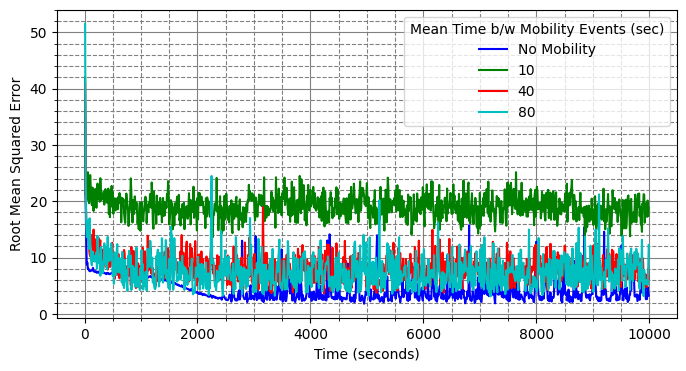
\includegraphics[width=\linewidth]{figures/design_space/nw_prox/rmsre_vs_time_num_agents_64.png}
  \caption{64 Clients.}
  \label{fig:mobility_N_64}
\end{subfigure}
\begin{subfigure}{0.48\textwidth}
  \centering
  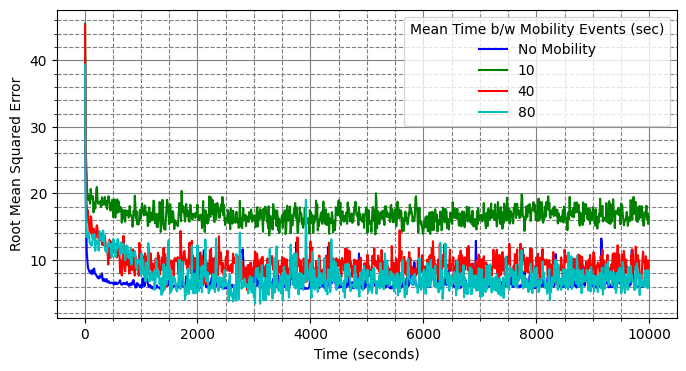
\includegraphics[width=\linewidth]{figures/design_space/nw_prox/rmsre_vs_time_num_agents_256.png}
  \caption{256 Clients.}
  \label{fig:mobility_N_256}
\end{subfigure}
\begin{subfigure}{0.48\textwidth}
  \centering
  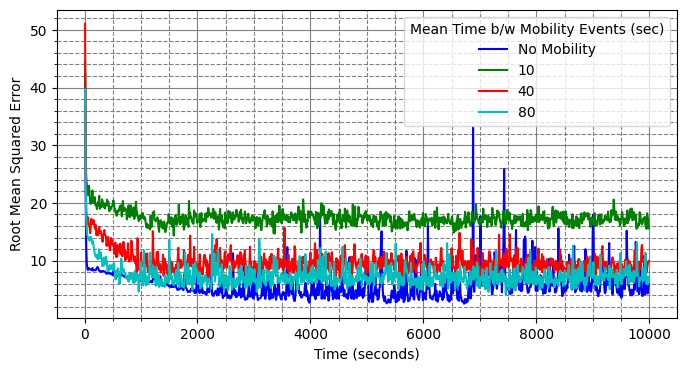
\includegraphics[width=\linewidth]{figures/design_space/nw_prox/rmsre_vs_time_num_agents_512.png}
  \caption{512 Clients.}
  \label{fig:mobility_N_512}
\end{subfigure}
\label{fig:mobility_nc_rmse}
\caption{Variation of RMSE over time for varying number of clients and varying degrees of client mobility.}
\end{figure}
For all scenarios with different number of clients, the RMSE in network latency estimation is the lowest for the case without mobility and increases progressively with more frequent mobility events per client. Hence, we conclude that the frequent changes in network connectivity for clients results in deterioration of RMSE of network latency estimation. Therefore, we propose an approach to eliminate this error in the following.

\subsubsection{Network Coordinate Proxy running on Edge Gateway}
Mobile devices invariably connect to the Internet via a nearby gateway node that runs on the Edge of the network e.g., local breakout \cite{localbreakout} for clients running on a 4G/LTE network. We assume the presence of a lightweight network coordinate proxy (NC Proxy) running on such gateway nodes, serving as the source of network coordinate information for the mobile clients connected to that gateway node. For a client that is connected to the Internet via a particular Edge gateway, all uplink and downlink traffic flows through that gateway, and it is located at a fixed access network latency from the client. Hence, the network latency between the client and an Edge site can be calculated by computing the sum of the network latency between the site and the Edge gateway and the access latency between the client and the gateway. Therefore, the network coordinate agent on mobile client computes its current coordinate by using the vector and adjustment fields of the gateway's coordinate, and adding the access latency to the height component of the gateway's coordinate. The access latency is monitored by periodic measurement from the gateway.
\par In this dissertation, we assume that the accuracte discovery of the network coordinate agent running on the current serving Edge gateway can be facilitated by a DNS-based mechanism. Such a mechanism for application-level resolution at the Edge has been already presented in the context of content-delivery networks \cite{hsu2020dns}. 

\section{Distributed End-to-End Monitoring}
The data-plane of applications using a platform service usually comprises multiple components, with each component performing a specific action, and incurring latency. The latency incurred by each such component adds toward the end-to-end latency of the application, which is that the developer of the application cares about. Hence, the end-to-end monitoring mechanism aims to provide the ability to monitor the end-to-end latency of the data-plane for a variety of applications running on different platform services. We propose to do so by measuring all individual component latencies independently. The collected metrics are then aligned with respect to time using their timestamps and summed up to compute the end-to-end latency. The end-to-end latency estimate can then be used to check whether the constraints specified by developer have been violated.  In the case of detecting a violation, the metrics of individual components is to be used for performing a root-cause analysis to detect the component latency which is resulting in the violation.

\subsection{Logical Components in the Monitoring Mechanism}
\label{sec:monitoring_logical}
\begin{figure}
\centering
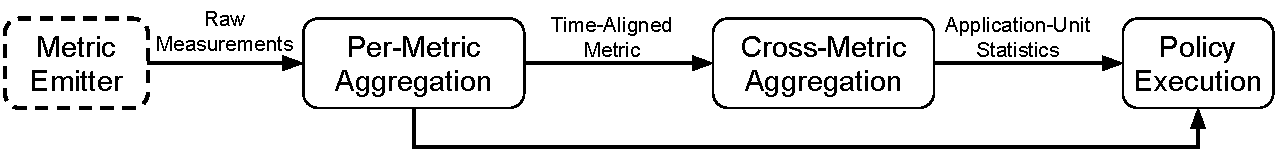
\includegraphics[width=\linewidth]{figures/design_space/monitoring/functions.pdf}
\caption{Logical components in the end-to-end monitoring mechanism and their interactions.}
\label{fig:monitoring_functions}
\end{figure}
\cref{fig:monitoring_functions} shows the logical functions that we propose as a part of the end-to-end monitoring mechanism. These functions perform all the necessary actions that are needed by typical platform services in order to continuously serve applications' desired quality of service.
\subsubsection{Metrics Emitter}
The Metrics Emitter component represents the platform service component generating measurements for a metric. The Metric Emitter could be the client library on a certain client device, an application instance running on an Edge site or a platform service component. 
\subsubsection{Per-Metric Aggregation}
The Metrics Emitter generates raw measurements, which are processed by the Per-Metric Aggregation function, that time-aligns the metric measurements while performing an aggregation as well to reduce the data volume. The output of the per-metric aggregation component is a stream of time-aligned measurement values which are emitted at regular intervals. The time interval between two consecutive measurements emitted by the per-metric aggregation component is equal to the bucket-size for the time-alignment. The timestamp associated with each aggregated time-aligned measurement values in the output stream is the start timestamp of the bucket.

\subsubsection{Multi-Metric Aggregation}
The Multi-Metric Aggregation function takes multiple time-aligned metrics at a particular timestamp as input and runs a platform-specific function to generate a value for that timestamp. 

\subsubsection{Policy Execution}
The control-plane policies then read the aggregated statistics generated by multi-metric aggregation as well as the time-aligned metrics to make decisions such as whether a certain application instance is undergoing performance violation and subsequently determining the root-cause of the violation.

\subsection{Design of the core components of end-to-end monitoring mechanism}
\subsubsection{Metrics Agent}
The Metrics Agent component is the one that is deployed alongside application and platform service components that need to be monitored, and acts as the interface between these components and the monitoring system. It is deployed as part of the client library or the application runtime or as a side-car of the platform service components. It provides interfaces for application and platform service components to register metrics and record observations for those metrics. 

\subsubsection{Metrics Server}
The Metrics Server is the component that holds the metrics reported by the various Metrics Agents. The Metrics Server serves two main functions - (i) it acts as a store for time-series measurement values, and (ii) an execution runtime for the aggregation and policy functions as discussed in \cref{sec:monitoring_logical}. 
\par The Metrics Server provides an interface similar to a Time-Series Data Base (TSDB). The Metrics Server provides a relational schema for defining metrics and their associated metadata. Having a relational schema also allows aggregation and policy logic to express queries based on metadata fields. The Metrics Server supports high-velocity ingestion of observations, and efficient querying including querying metric values from the past.
\par The Metrics Server supports platform-specific functions to be executed over the monitoring data that is stored in its data store. It allows the aggregation and policy functions to query metrics using their metadata fields. Once the identifier for a particular metric is known, the Metrics Server allows queries to fetch most recent as well as historical measurements recorded for that metric.

\subsection{Metrics of Interest}
We consider the following metrics of interest for quantifying the \textit{goodness} of the various design choices for implementing the end-to-end monitoring mechanism.
\begin{itemize}
\item \textbf{Monitoring Traffic through WAN. } The large number of application and platform-service entities continuously processing data and generating performance metrics would present a large volume of data to be fed into the monitoring system. The amount of traffic sent through the WAN needs to be minimized for the mechanism to be scalable.
\item \textbf{Response Time to Violation. }The time taken by the monitoring subsystem (including the Policy) to detect a significant change in a metric defines the responsiveness of the platform service to alleviate a potential violation. Hence, we intend to minimize the response time of the monitoring mechanism to detect a violation.
\item \textbf{Resource Requirements of Metrics Server. } The CPU and memory usage of the monitoring components need to be low so that instances of Metrics Agents and Metrics Servers can be hosted on Edge resources. A high resource requirement would mean that resources that could have been used for the data-plane of platform services would need to be devoted to monitoring, which would result in worse utilization of scarce Edge resources.
\end{itemize}


\subsection{Design Choices}
We explore two design choices for organizing the logical functions discussed in \cref{sec:monitoring_functions} over a geo-distributed infrastructure. We enumerate the design choices in the following.

\subsubsection{Fully Centralized Approach}
In the fully centralized approach, all of the monitoring functionalities, ranging from the Per-Metric Aggregation to the Policy Execution are hosted in the Cloud. In this approach, the metrics are emitted by Metric Emitters located at the Edge within Metrics Agents, and the raw measurements traverse through the WAN to get to the following functions. 

\subsubsection{Distributed Approach}
In this approach, the Metric Emitters are located within Metrics Agents, which is same as the centralized approach. In addition to that, the Per-Metric Aggregation function for a given metric is co-located with the Emitter for that metric. In this way, raw measurements are not sent through the WAN, rather it is the time-aligned metric stream that is sent to the Cross-Metric Aggregation function. This approach is able to work on a large scale because the properties of the Per-Metric Aggregation function, such as bucket size, does not change frequently.

\begin{comment}
\subsubsection{Distributed Approach 2}
This approach is a variant of the Distributed Approach 1, wherein, the Cross-Metric Aggregation component is also moved to the Edge. Typical control-plane policies such as violation detection operate independently on a specific unit of the application, such as a specific application pipeline instance or publish-subscribe topic. Hence it is possible to host multiple instances of cross-metric aggregation component for different application units at multiple Metrics Servers running on the Edge. All the metrics corresponding to a specific application unit will need to be sent to the Metric Server that hosts that application unit's cross-metric aggregation function. 
\end{comment}

\subsection{Evaluation of Candidate Design Choices}
We evaluate the aforementioned candidate design choices for implementing the end-to-end monitoring mechanism and present results in this section. In our evaluations, we consider 1 application unit which has a number of distributed system entities associated with it. All these system entities generate measurements to 1 metric at a certain measurement frequency. Each metric is time-aligned using a specific bucket-size wherein the metrics falling inside a bucket are summarized by taking an average. The time-aligned summaries of each metric are sent to the Multi-Metric Aggregation which checks if all the metric summaries for the current bucket have been received, and if so, passed them to the policy execution. 
\par In our experiments, the Metric Emitters are located on the Edge, while the Multi-Metric Aggregation is deployed in the Cloud. Per-Metric Aggregation can run either on the Edge alongside Metric Emitters or in the Cloud based on the design choice being evaluated. 

\begin{figure}
\centering
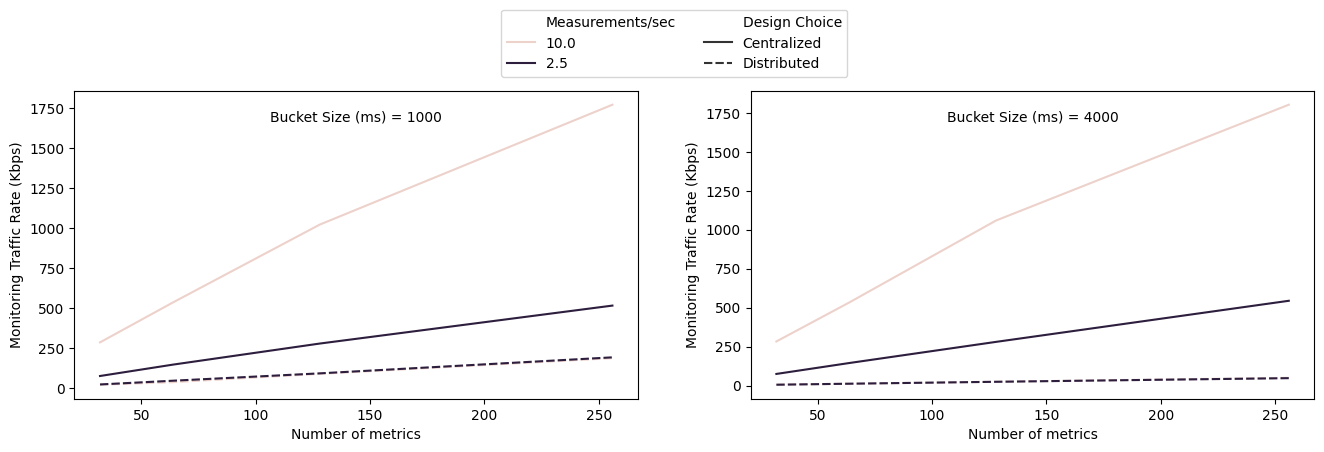
\includegraphics[width=\linewidth]{figures/design_space/monitoring/nw_usage.png}
\caption{Network bandwidth usage of the design choices for end-to-end monitoring mechanism.}
\label{fig:monitoring_nw_usage}
\end{figure}
\cref{fig:monitoring_nw_usage} shows the network bandwidth usage by the two design choices we evaluate for the end-to-end monitoring mechanism. We perform the evaluation for two bucket sizes - 1 second and 4 seconds - and two per-metric measurement rates - 2.5 and 10 measurements per second. For all four of these configurations, we see that the Distributed design choice incurs less network traffic between the Edge and the Cloud as compared to the Centralized design choice. Furthermore, the traffic consumed by Distributed approach does not change with different per-metric measurement rates because it only sends a summary of measurements (average) at an interval of 1 bucket size. These results show that the Distributed design choice is a more scalable one in terms of network bandwidth usage.

\begin{figure}
\centering
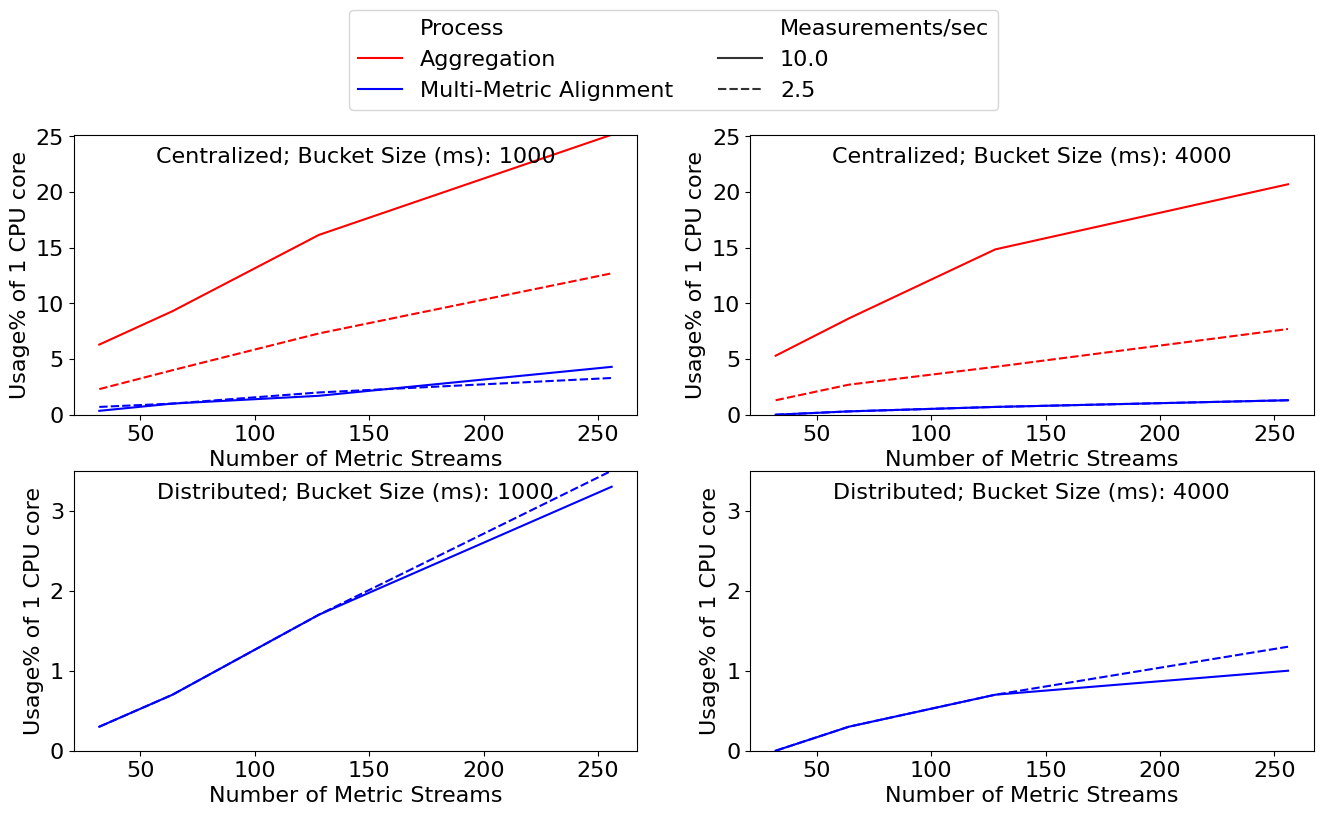
\includegraphics[width=\linewidth]{figures/design_space/monitoring/cpu_usage.png}
\caption{CPU usage of each component in various design choices of the end-to-end monitoring mechanism.}
\label{fig:monitoring_cpu_usage}
\end{figure}
\cref{fig:monitoring_cpu_usage} shows the CPU usage of the various components involved in the monitoring mechanism, when deployed in the evaluated design choice configurations. In the centralized approach, when all raw measurements are sent directly to the Cloud, the Aggregation component consumes a high amount of CPU to process the incoming measurements. The CPU usage naturally grows with the number of metrics and the rate of measurements reported for each individual metric. The Multi-Metric Alignment component, however, is much less resource-intensive relatively. In the Distributed approach, since the Per-Metric Aggregation component is co-resident with the Metrics Emitter, the CPU load for aggregating metrics is spread over all the geo-distributed Emitters, and hence we don't show it in the figure. The evaluation results show that in terms of CPU usage, the Distributed design choice is more scalable.

\begin{figure}
\centering
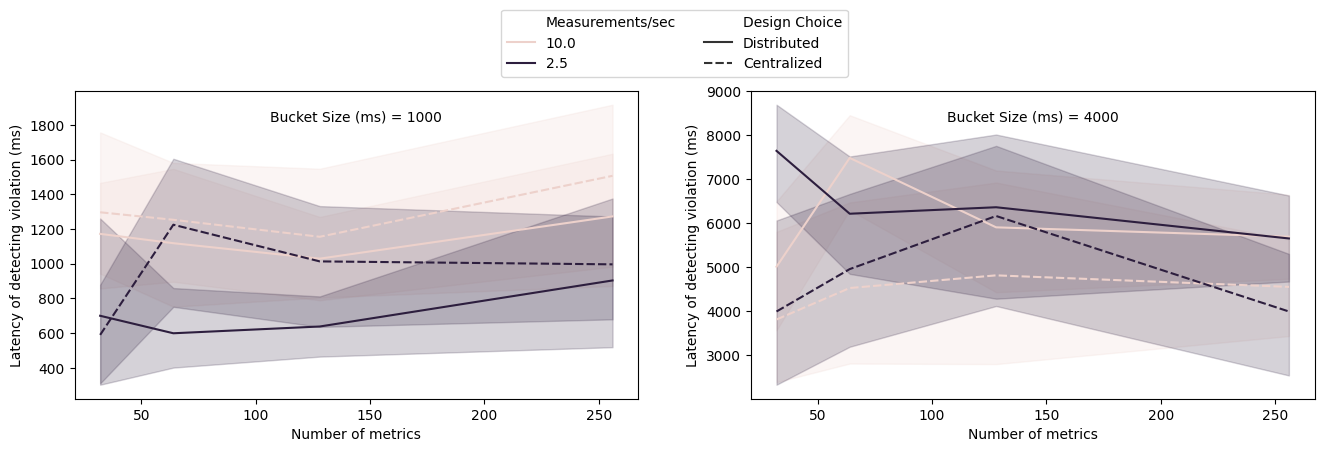
\includegraphics[width=\linewidth]{figures/design_space/monitoring/response_time.png}
\caption{.}
\label{fig:monitoring_response_time}
\end{figure}
Finally, \cref{fig:monitoring_response_time} shows the variation of the latency of detecting a violation with the two evaluated design choices. The results show that both Centralized and Distributed Approaches have a similar behavior in terms of the violation detection latency, with the latency being dependent only on the bucket size. 
\par Hence, we conclude that the Distributed Design choice is not only more scalable in terms of network and CPU usage, but it also provides the same response time as the Centralized approach. Hence, we use it in implementing the end-to-end monitoring mechanism.
    %\chapter{ePulsar: Topic-based publish-subscribe system with end-to-end latency guarantees}
\label{sec:epulsar}

Applications such as navigation control of Unmanned Aerial Vehicles (UAVs) and collaborative perception for autonomous driving need to support a large number of clients, retaining high throughput and low latency communication. The synchronization decoupling provided by publish-subscribe (pub-sub) systems \cite{manyfaces, PubSubForMultiplayerGames} makes them an ideal messaging middleware for supporting these applications. Typically, pub-sub systems consist of ``broker'' \textit{middleware nodes} that are responsible for message exchange  between ``producers'' and ``consumers'' of data in the system. Brokers manage ``topics'', where a topic acts like a message queue to which producers publish messages, and consumers receive messages from it. Popular pub-sub systems such as Apache Kafka and Pulsar are commonly used for supporting low latency and high throughput messaging for cloud applications. % For instance, publish-subscribe 
Pub-sub systems have been shown to be suitable for sharing game state updates in MMOGs  \cite{PubSubForMultiplayerGames}, swarm synchronization for autonomous robots (drones)~\cite{flynetsim}, and data distribution for large-scale stream processing \cite{7164934}. However, contemporary applications such as large scale IoT, and Unmanned Aerial Vehicle (UAV) coordination pose latency constraints that make cloud-based publish-subscribe system deployments unsuitable due to the high WAN latency between clients (producers and consumers) and middleware (broker) nodes. Given the proximal nature of Edge resources, they can be utilized for hosting pub-sub middleware nodes close to clients and thereby provide low end-to-end message delivery latency.
\par However, adapting state-of-the-art cloud-based pub-sub systems like Kafka and Pulsar to a geo-distributed Edge infrastructure poses peculiar challenges. Such systems typically are topic-based and they partition topics among brokers by computing a consistent-hash of the topic name. Consistent hashing ensures even distribution of load among brokers - that is key to manageable end-to-end latency in datacenters where the network topology is more or less homogeneous. However, in Edge infrastructure, the physical location and network connectivity of a client have a significant impact on the client-broker network latency, and latency-agnostic consistent hashing does not account for network proximity. In addition, client mobility requires constant adaptation of the broker hosting a given topic so as to continuously provide low end-to-end latency for that topic. The network infrastructure itself could experience changes (e.g., increased latency between servers) that might affect end-to-end latency. Finally, due to the capacity constraints and limited statistical multiplexing at Edge sites, load-aware topic partitioning is important to avoid workload hotspots and minimize end-to-end latency \cite{khare2018scalable}.

\par To address the above challenges, we design a novel \textit{edge-centric control plane architecture} for pub-sub systems.  The elements of this architecture include the following features:
\begin{enumerate}
\item \epulsar leverages the Network Proximity Estimation mechanism for its latency and load-aware broker selection policy that assigns topics to brokers to ensure that end-to-end message delivery constraint of each topic is satisfied. 
\item \epulsar leverages the End-to-End Monitoring mechanism to monitor client and broker network proximity metrics as well as per-topic traffic characteristics and aggregates that information for each topic. The per-topic aggregates of monitoring data are then processed by control plane policies for detecting if a topic needs to be migrated away from the current hosting broker to alleviate latency violation.
\end{enumerate}
The roadmap of this chapter is as follows. \cref{sec:epulsar_background} presents the necessary background for this chapter. \cref{sec:epulsar_arch} presents the architecture of \epulsar{}. \cref{sec:epulsar_nw_prox} describes how \epulsar{} uses the Network Proximity Estimation mechanism for estimating the end-to-end message delivery latency for broker selection. \cref{sec:epulsar_dist_mon} presents \epulsar's use of the End-to-End Monitoring mechanism for detecting and alleviating violations of end-to-end message delivery latency constraint. \cref{sec:epulsar_impl} presents implementation details in \epulsar{} and \cref{sec:epulsar_evals} presents results of experimental evaluation of \epulsar{}. Finally, \cref{sec:epulsar_conclusion} presents concluding remarks.

\section{Basics of Publish-Subscribe}
\label{sec:epulsar_background}
\subsection{Publish-Subscribe Communication Model}
The publish-subscribe communication pattern is used widely across the current software ecosystem \cite{manyfaces}, especially when there are going to be a large number of communicating entities. In the publish-subscribe pattern, there are two classes of communicating entities for a given type of data - \textit{publishers} and \textit{subscribers}. As their name indicates, publishers generate data that is consumed by subscribers. The main motivation for using a publish-subscribe system is that it does not require the publishers to know who the subscribers are so that the data can be sent to them. Instead, a typical publish-subscribe system allows the subscribers to express their interest in a certain type of data, and whenever a publisher generates a data-item that matches a subscriber's interest the subscriber is notified. This data exchange is done by using a set of middleware nodes that form the core of the publish-subscribe system, and are typically called \textit{brokers}. A publisher sends each data-item that it generates to a broker, that then determines the set of subscribers who should be notified of this data-item, and sends the data-item to them. By relying on brokers, a publish-subscribe system decouples the data producers and consumers. This decoupling can be categorized into three classes:
\begin{itemize}
\item \textbf{Space decoupling}: The communicating entities do not need to know about each other. In other words, the publishers do not need to hold a reference of the subscribers and similarly, subscribers do not need to hold a reference of the publishers. They simply connect to the broker and send/receive messages from it.
\item \textbf{Time decoupling}: For a specific message, the publisher generating it and the subscribers consuming it do not need to be active at the same time. Subscribers are notified of a messages that matches its interest even though it was published when the subscriber was not connected to the publish-subscribe system.
\item \textbf{Synchronization decoupling}: Publishers are not blocked for producing messages by the subscribers consuming them. Subscribers can keep performing other tasks in parallel while they are asynchronously notified of incoming messages from publishers. 
\end{itemize}
There are three broad categories of publish-subscribe systems \cite{eugster2003many}:
\begin{itemize}
\item \textbf{Topic-based publish-subscribe}: In topic-based publish-subscribe systems, all communication between entities is done through ``topics'', that is an abstraction similar to a message queue or a channel. Publishers using the ``publish()'' function to send a message to a given topic, while subscribes used the ``subscribe()'' function to receive messages from the topic.
\item \textbf{Content-based publish-subscribe}. These systems allow more expressiveness than topic-based systems by allowing subscribers to express interest in the messages they will receive based on the actual content of messages. Subscribers provide predicates to filter the messages that they are interested in receiving.
\item \textbf{Type-based publish-subscribe}. Type-based publish-subscribe systems allow subscribers to specify which messages they want to receive based on the ``type'' of the message. 
\end{itemize}
In this project, we are going to be considering a topic-based publish-subscribe system because a significant portion of popular and commercially available publish-subscribe systems are topic-based. Due to their simplicity of interest matching, they are easier to implement and are generally more efficient than the other categories. 

\subsection{Data Delivery Guarantees}
Applications using publish-subscribe systems typically expect certain functional guarantees on data delivery from publishers to subscribers. The two most common properties that applications require are \textit{exactly-once message delivery} and \textit{message persistence}. This subsection discusses these guarantees, that \epulsar{} aims to provide as well.
\subsubsection{Exactly-once Message Delivery}
Each data subscriber expects every message that was successfully published (and acknowledged) to be received only once. A message can neither be dropped nor delivered more than once. This approach requires that (1) each message has a unique identifier that distinguishes it from other messages; (2) publishers are able to re-send messages that were not successfully published; (3) brokers are able to perform de-duplication of the same message that was published multiple times; and (4) subscribers track the last message that they received, and can query the broker for any newer messages that it might have for the given subscriber. 

\subsubsection{Message Persistence}
A typical distributed system has several communicating entities, all of which cannot be online at the same time. A publish-subscribe system should be able to tolerate the disconnection of subscribers at a time when publishers are publishing messages. A subscriber client should be able to reconnect at a later point in time and be able to receive the pending messages, which requires that the publish-subscribe middleware not only maintains a log of the messages that were published, but also keeps track of which messages have been successfully delivered to each subscriber so that a subscriber is only sent the unread messages when it reconnects.
\subsection{Message Delivery Latency Guarantee}
In addition to the correctness of sending and receiving messages that are provided by data delivery guarantees, emerging applications, such as drone-swarm coordination and autonomous or assisted driving, require that the time spent from the generation of the message, to it being received by the publish-subscribe middleware, till the time when it is received by all the relevant subscribers should be low and bounded. The message delivery latency is composed of (1) communication latency from the publisher to the publish-subscribe middleware; (2) latency incurred in processing and persisting the message on the middleware; and (3) communication latency from the middleware to the subscribers. In a typical scenario, multiple publishers communicate with multiple subscribers, hence the message delivery latency guarantee has to be satisfied for all possible pairs of publishers and subscribers.

\section{Architectural Components of ePulsar}
\label{sec:epulsar_arch}
\subsection{Data Plane Components}
\subsubsection{Clients}
Clients are geo-distributed and each client is a publisher or a subscriber of a topic. A publisher sends messages to the broker hosting its topic, while a subscriber receives messages published to its topic as notifications.
\subsubsection{Brokers}
Brokers are the components of any publish-subscribe system responsible for message exchange between producers and consumers. In \epulsar, brokers are deployed on geo-distributed Edge sites. Brokers are also associated with another software component called BookKeeper, that acts as the high-performance storage layer. BookKeeper nodes, called \textit{bookies}, persist messages for each topic so that older messages can be retrieved in the event of a broker failure or broker migration.
\subsection{Control Plane Components}
\subsubsection{Metrics Store}
The Metrics Store receives monitoring metrics from clients and brokers pertaining to resource consumption of brokers, message rates on topics and network proximity between clients and brokers. This monitoring data is accessed by the control-plane for making dynamic topic placement decisions through the broker selection and violation detection policies, that are described next.
\subsubsection{Broker Selection Policy}
The broker selection policy of \epulsar{} assigns topics to brokers in a latency-aware manner such that the end-to-end latency of data delivery from the producer to broker and finally to the consumer is bounded by the latency threshold provided for the topic. 
\begin{figure}[h]
\centering
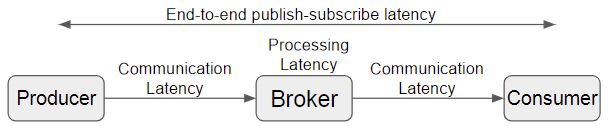
\includegraphics[width=0.75\columnwidth]{figures/epulsar/e2e_latency_breakdown.JPG}
\label{fig:e2e_latency_breakdown}
\caption{Breakdown of end-to-end message delivery latency for a producer-consumer pair.}
\end{figure}
As shown in \cref{fig:e2e_latency_breakdown}, the end-to-end message delivery latency is made up of the communication latency between the producer and serving broker, the latency of handling the message on the broker (potentially persisting it on durable storage in the case of a persistence topic), and the communication latency from the broker to the consumer. The sum of all these component latencies needs to be below the latency threshold. This constraint needs to be satisfied for each producer-consumer pair of the given topic, that may have disparate connectivity to the serving broker compared to other producer-consumer pairs. Hence the broker selection policy needs to select a broker for hosting a topic that is (1) in network proximity to the clients of the topic to ensure low communication latency; and (2) is not overloaded to ensure low processing latency.

\subsubsection{Violation Detection Policy}
The violation Detection Policy of \epulsar{} is used to check whether an existing topic in the publish-subscribe system has its end-to-end message delivery latency constraint violated. This computation is done for each topic independently. Since publisher and subscriber clients of a topic can be connected at different points in the network topology, the worst-case message delivery latency is incurred for the publisher-subscriber pair that are the furthest from the broker. Thus, all possible publisher-subscriber pairs have to be analyzed to check for violations.
\par The worst-case message delivery latency for a topic is the sum of the maximum network latency from any publisher to the broker, the maximum network latency from the broker to any subscriber, and the per-message processing latency on the broker. The worst-case message delivery latency of a topic is compared against the topic-specific threshold, and if the observed latency exceeds the threshold, a violation is detected, and the control-plane triggers the migration of the topic to another broker that can satisfy the latency constraint.
%The first two components is calculated using the clients' network coordinates, while the processing latency is estimated by using a profile of the broker's data-plane through offline profiling.
\subsection{Use of Proposed Mechanisms in Control Plane}
\epulsar{}'s control plane utilizes the Network Proximity Estimation mechanism to estimate the worst-case message delivery latency for a given topic. This mechanism is able to estimate the communication component of the message delivery latency, while \epulsar{} relies on an offline profile of its broker's data plane for estimating the processing latency. This mechanism is used both for (1) determining whether a particular candidate broker will be able to satisfy the worst-case message delivery latency constraint, given the network proximity information between the clients and the candidate broker, and (2) detecting a violation of the worst-case message delivery latency constraint. The clients' network proximity to the current serving broker is used to compute the observed worst-case message delivery latency, that is then compared against the topic-specific threshold.

\section{End-to-End Latency Estimation using Network Proximity Mechanism}
\label{sec:epulsar_nw_prox}
\begin{figure}[h]
\centering
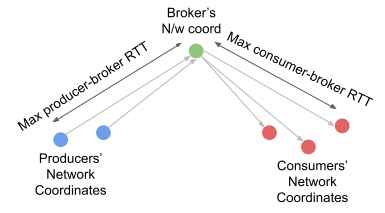
\includegraphics[width=0.75\columnwidth]{figures/epulsar/nw_coord_latency.png}
\label{fig:nw_coord_latency}
\caption{Illustration of the use of network coordinates for computing the worst-case message delivery latency for a given topic. Network coordinates can be used to compute the communication component of the message delivery latency. Since all publisher-subscriber pairs communicate via the broker, computing the maximum network latency from the publishers to the broker and that from the broker to the subscribers suffices to compute the worst-case communication latency across all publisher-subscribe pairs.}
\end{figure}
\subsection{Deployment of Network Coordinate Agents}
Estimating the network latency between every client and broker pair requires that all of those entities have an associated network coordinate, such that by computing the Euclidean distance between the coordinates of two nodes, one can compute the communication latency between them. \epulsar{} co-locates one instance of the Network Coordinate Agent with each broker, such that the network coordinate of the agent represents the network proximity information of the broker. Clients that are not mobile (e.g., connected to a wired network) also run a Network Coordinate Agent instance and use the agent's coordinate as their own. To handle mobile clients, \epulsar{} relies on a network of Edge Gateways that each run a Network Coordinate Agent. Each client discovers the current serving Edge Gateway using a DNS-like discovery mechanism, records the network round-trip time to the Gateway and computes its own network coordinate from the network coordinate of the Gateway and the measured RTT to Gateway. The deployment is illustrated in \cref{fig:epulsar_nc_deployment}. The network coordinates of all these system entities is utilized by the broker selection and violation detection policies for estimating the communication component of the end-to-end message delivery latency. 
\begin{figure}[h]
\centering
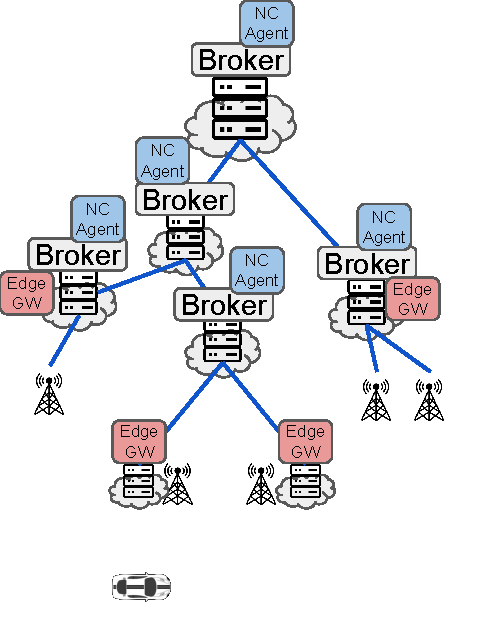
\includegraphics[width=0.5\columnwidth]{figures/epulsar/nc_agent_deployment}
\label{fig:epulsar_nc_deployment}
\caption{Illustration of the deployment of network coordinate agents in \epulsar{}.}
\end{figure}

\begin{table}[t]
	\center
	%\begin{adjustbox}{width=0.8\columnwidth,center}
		\begin{tabular}{ |c|c| } 
			\hline
			\textbf{Notation} & \textbf{Definition}\\ 
			\hline
			$t$ & topic\\
			$P\left( t \right)$ & producers of topic $t$\\
			$C\left( t \right)$ & consumers of topic $t$\\
			$L_{th}\left( t \right)$ & end-to-end latency constraint for topic $t$\\
			$B\left[ t \right]$ & broker hosting topic $t$\\
			$NC\left( i \right)$ & network coordinate of entity $i$\\
			$\overline{NC}\left( I \right)$ & centroid network coordinate of entities in $I$\\
			$d\left( nc_1, nc_2 \right)$ & distance between network coordinates\\
			$W\left( t \right)$ & Deviation of client NC from centroids of topic $t$\\
			$W\left( t \right)$ & Deviation of client NC from centroids of topic $t$\\
			$E\left( t \right)$ & Worst-case end-to-end latency for topic $t$\\
			$PROC \left( t \right)$ & Processing latency at broker for topic $t$\\
			\hline
		\end{tabular}
	%\end{adjustbox}
	\caption{Notations used.}\label{table:notations}
\end{table}

\subsection{Broker Selection Policy}
The set of publishers and subscribers for a topic $t$ are denoted by $P \left( t \right)$ and $C \left( t \right)$ respectively. The worst-case message delivery latency for topic $t$ when served by broker $b$ is represented as shown in \cref{eq:e2e_latency}.
\begin{equation}
W\left( t, b \right) = \max\limits_{p \in P\left( t \right)} d \left( NC \left( p\right), NC \left( b\right) \right)/2 + \max\limits_{c \in C\left( t \right)} d \left( NC \left( c\right), NC \left( b\right)\right)/2 + PROC \left( t \right)
\label{eq:e2e_latency}
\end{equation}
\cref{eq:e2e_latency} is used by the broker selection policy to estimate the worse-case message delivery latency that a given broker can provide for a given topic. The broker selection policy is shown in \cref{algo:broker_sel_algo}. For each topic that needs to be placed on a broker, the policy finds the set of candidate brokers that can satisfy the message delivery latency constraint (line 3-4). Next, the policy ranks the topics in increasing order of the number of possible candidates for each topic and starts broker selection in that order (lines 5-6). The aim of the policy is to successfully place as many topics as possible. Next, if a particular broker can host a given topic without being overloaded, the topic is assigned to that broker (lines 7-9). 
\begin{algorithm}
\caption{Broker selection policy algorithm. Inputs are $T$ (set of topics to place on brokers), current topic-to-broker mapping $B$, and $M$ (monitoring data)}\label{algo:broker_sel_algo}
\begin{algorithmic}[1]
\Procedure{SelectBroker}{$T, B, M$}
\State $F \gets dict\left(\right)$
\For{$t \in T$}
    \State $F \left[ t \right] \gets get\_feasible\_brokers\_by\_latency \left( t , M\right)$
\EndFor
\State $\text{sort } T \text{ by increasing } |F \left[ t \right]|$
\For {$t \in T$}
    \For {$b_{cand} \in F \left[ t \right]$}
        \If{$can\_host \left( b_{cand}, t, B, M\right)$} \Comment{no broker overload}
            \State $B \left[ t \right] \gets b_{cand}$
            \State break
        \EndIf
    \EndFor
\EndFor
\State $\text{return } P$
\EndProcedure
\end{algorithmic}
\end{algorithm}

\subsection{Violation Detection Policy}
The Violation Detection Policy is invoked periodically, that iterates over all the topics currently in the system and checks if any one of them is undergoing latency violation (lines 4-5). If a topic is experiencing end-to-end latency violation, it is added to the set of topics that need to be migrated to a better broker (line 6). Next the policy checks if any broker is overloaded due to too many topics (line 7). In case there is a broker that is overloaded, the policy fetches the topics that are best candidates for migrating out of the overloaded broker (line 9), and adds it to the set of topics to be migrated. Then the policy calls the topic-placement module that uses \cref{algo:broker_sel_algo} for selecting the target broker for hosting each topic (line 11). If the chosen target broker is not the same as the current broker, a topic migration is triggered (lines 14-16).
\begin{algorithm}
\caption{Violation Detection Policy algorithm. Inputs are $B_0$ (initial topic partitioning) and $M$ (monitoring data)}\label{viol_detection_algo}
\begin{algorithmic}[1]
\Procedure{PerformRepartitioning}{$B_0$, $M$}
\State $R \gets \{\}$ \Comment{set of migration commands}
\State $T_{migr} \gets \{\}$ \Comment{topics to migrate from curr broker}
\For{$t \in B_0.topics$}
    \If{$latency\_violated \left( t \right)$}
        \State $T_{migr} \gets T_{migr} \cup \{ t \}$
    \EndIf
\EndFor

\State $B_{overload} \gets get\_overloaded\_brokers \left( B_0, M \right)$
\For{$b \in B_{overload}$} \Comment{resource-based detection}
    \State $T_b \gets get\_topics\_to\_migrate\left(b, B_0, M\right)$
    \State $T_{migr} \gets T_{migr} \cup T_b$
\EndFor
\State $B \gets PlaceTopics \left( T_{migr}, B_0, M \right)$ 

\State $R \gets \{\}$ \Comment{set of re-partitioning commands}
\For {$t \in B_0.topics$}
    \If {$B\left[ t \right] \neq B_0 \left[ t \right]$}
        \State $R \gets R \cup \{ \left( t, B_0 \left[ t \right], B \left[ t \right]\right) \}$ \Comment{add previous broker and new broker}
    \EndIf
\EndFor
\State $execute\_reconfigs \left( R \right)$ 
\EndProcedure
\end{algorithmic}
\end{algorithm}

\section{Distributed Monitoring in ePulsar}
\label{sec:epulsar_dist_mon}
\subsection{Distribution of Monitoring Components over Infrastructure}
Each client in \epulsar{} hosts a Metric Agent that monitors the client's network coordinate. Each broker hosts a Metric Agent that monitors its network coordinate and the message rate for each topic. These metrics agents perform Per-Metric Aggregation of each metric with a bucket size of 5 seconds, computing the average over all the measurements in each bucket. 
\par Each broker hosts the Metrics Server along with it. For each topic that is hosted on a given broker, all clients of that topic report their metric aggregates to the Metrics Server hosted on that broker, that performs an aggregation of the network coordinates as discussed in \cref{sec:epulsar_mon_aggr}. The aggregated metrics are then reported to the control plane's Metric Store to be used by violation detection and broker selection policies.

%performs monitoring of the network coordinates of clients and broker as well as the message rate of each topic on the broker that is hosting the topic. Since all the relevant metrics of a given topic are present on the broker itself, it can aggregate the topic's metrics to reduce the amount of data that needs to be sent to the Metrics Store via the wide-area network.

\subsection{Monitoring Data Aggregation Logic}
\label{sec:epulsar_mon_aggr}
\epulsar{} reduces the amount of per-topic monitoring data sent to the Metric Store by aggregating the network coordinates of multiple clients of each topic. For each topic $t$ that is hosted on broker $b$, \epulsar{} reports the following aggregate statistics to the Metric Store. \cref{table:notations} provides a summary of notations used.
\begin{itemize}
\item \textbf{Producer and Consumer Centroid.} The centroids of producers' and consumers' network coordinates provide an approximate network \textit{location} of a topic's clients. We compute the centroid producer coordinate $\overline{NC_P}\left( t \right)$ and centroid consumer coordinate $\overline{NC_C}\left( t \right)$ as follows.
\begin{equation*}
\overline{NC_P}\left( t \right) = \overline{NC} \left( \{ i : i \in P\left( t \right) \} \right)
\end{equation*}
\begin{equation*}
\overline{NC_C}\left( t \right) = \overline{NC} \left( \{ i : i \in C\left( t \right) \} \right)
\end{equation*}
\item \textbf{Maximum Deviation from Centroids.} To account for the loss of fine-grained network coordinate information due to aggregating them as centroids, \epulsar{} sends the maximum deviation of the clients' coordinates from their corresponding centroid. We denote this as $W \left( t \right)$ and it is computed as shown below.
\begin{equation*}
W \left( t \right) = \max\limits_{p \in P\left( t \right)} d \left( NC \left( p\right), \overline{NC_P}\left( t \right)\right)/2 + \max\limits_{c \in C\left( t \right)} d \left( NC \left( c\right), \overline{NC_C}\left( t \right)\right)/2
\end{equation*}
\item \textbf{Worst-case Communication Latency.} For each topic $t$, we compute the worst-case communication latency across all producer-consumer pairs. We denote this as $E \left( t \right)$ and it is computed as follows. 
\begin{equation*}
E \left( t \right) = \max\limits_{p \in P\left( t \right)} d \left( NC \left( p\right), NC\left( B\left[ t \right] \right) \right) / 2 + \max\limits_{c \in C\left( t \right)} d \left( NC \left( c\right), NC\left( B\left[ t \right] \right) \right) / 2
\end{equation*}
This information is used to determine whether the current broker, denoted by $B\left[ t \right]$ is meeting the topic's end-to-end pub-sub latency threshold.
\end{itemize}

\par One key point to take note of is that the volume of per-topic monitoring data generated is independent of the number of clients using that topic. Given the high heterogeneity of broker and client network locations in a geo-distributed setting, the above aggregation technique significantly reduces monitoring data traffic. By contrast, a naive approach that records the network coordinates of all clients would incur network traffic proportional to the number of clients of each topic. However, the monitoring data used by \epulsar{}'s broker selection policy does not contain individual client network coordinates, but rather the centroids of producer and consumer clients' network coordinates. Hence, \cref{eq:e2e_latency} in the Broker Selection Policy needs to be updated to use centroid coordinates as shown in \cref{eq:e2e_latency_w_centroids}.
\begin{equation}
\label{eq:e2e_latency_w_centroids}
W \left( t, b\right) = d \left( \overline{NC_P} \left( t \right), NC \left( b \right) \right) + d \left( \overline{NC_C} \left( t \right), NC \left( b \right) \right) + W \left( t \right) + PROC \left( t \right)
\vspace{-0.05in}
\end{equation}

\section{Implementation of \epulsar{}}
\label{sec:epulsar_impl}
\epulsar{} is implemented by extending Apache Pulsar v2.2.1. We chose Pulsar as the base system because of the strong data-plane semantics that it offers and also because topic migrations in Pulsar are much more agile than in Apache Kafka. However, Pulsar, like Kafka, is designed for datacenters and bundles topics together for monitoring and placement on brokers. This bundling is done for reducing the amount of metadata that it has to maintain. \epulsar{} needs to independently manage each topic, and hence, we restrict the maximum number of topics in a bundle to be 1. When more than one topics are mapped to a bundle, it results in the bundle being split into two new bundles, each with one topic. By inheriting the concept of bundles from Pulsar, \epulsar{} is able to re-use the bundle-centric monitoring and broker selection in Pulsar, while being able to manage each topic independently.
\par The control plane policies of broker selection and violation detection are implemented in the Load Manager module of Pulsar. We replace the off-the-shelf Load Manager of Pulsar, that aims at even distribution of workload and prevention of hotspots, with an edge-centric implementation that takes communication latency into account as well. \epulsar{} inherits from Pulsar the use of a ZooKeeper instance as the Metrics Store, that is also used for storing configuration information about the system, e.g., topic ownership of each broker, cluster membership, etc. The monitoring data is queried by the Load Manager module periodically every 5 seconds to detect violations and compute better brokers for topics that are undergoing latency constraint violation.

\par Brokers in \epulsar{} run on Edge sites along with cloud datacenters. The control plane component of Pulsar, i.e., Load Manager, runs on one of the brokers at a time, that serves as the Leader broker of the cluster. In \epulsar{} the Leader broker is forced to be one that is deployed in a datacenter for better availability. Hence, \epulsar{} has a centralized control-plane located in a cloud datacenter. The ZooKeeper instance that serves as the Metrics Store is co-located in the same datacenter as the Leader broker running the Load Manager module. Clients connect to the publish-subscribe infrastructure via various access media, e.g., cellular (4G LTE), WiFi or wired networks. All entities in the publish-subscribe system, including brokers and clients periodically (every 5 seconds) query their network coordinate, either from the Network Coordinate Agent co-located with them (in the case of brokers and static clients) or from the serving Edge Gateway (in the case of mobile clients) and report it to the monitoring mechanism.

\section{Evaluations}
\label{sec:epulsar_evals}
In this section, we present a set of evaluations to demonstrate the efficacy of the proposed mechanisms in enabling an edge-centric latency-aware control plane for a geo-distributed publish-subscribe system \epulsar{}. Specifically, we aim to prove the following hypotheses through experimentation.
\begin{enumerate}
\item Incorporating network proximity information in the broker selection policy allows the satisfaction of per-topic latency constraints. Aggregation of client network coordinates does not impair the quality of the broker selection decision.
\item Distributed monitoring results in monitoring overhead reduction.
\item \epulsar{} is able to meet the end-to-end latency constraints for exemplar applications.
\end{enumerate}
We verify the above hypotheses using two main methods: (1) microbenchmarks that analyze different components of \epulsar's architecture in isolation; (2) end-to-end evaluations of the UAV Swarm application scenario consisting of realistic infrastructure topology and client workload.

\subsection{Evaluation Scenario}
\label{sec:epulsar_eval_scenario}
We evaluate \epulsar{} under realistic infrastructure and subscription patterns. We consider the following evaluation scenario from which we design microbenchmarks and end-to-end experiments.
\par A UAV swarm consists of multiple drones that move together to accomplish a given task. The swarm contains a leader UAV and the rest of the UAVs are followers. Each swarm follows a Random Waypoint mobility model \cite{rwp}.\\
\textbf{Subscription Pattern. } The leader UAV sends movement commands to the followers through a topic called \textit{follow\_leader}. The followers communicate information extracted from onboard sensors to the leader via a topic \textit{sensor\_data}. The E2E pub-sub latency constraint is set at 40 ms.\\
\textbf{Infrastructure. } We consider a city-wide cellular network equipped with Edge resources, where UAVs use 4G-LTE as the communication medium. We assume that the city is divided into multiple \textit{Mobile Edge Computing (MEC)} zones, each with a single edge site. The locations of the edge sites is determined via k-means clustering of the cell tower locations \cite{wang2019edge} of Atlanta~\cite{cellmapper}. The Edge sites communicate with each other via a city-level switch, with inter-site RTT of 30 ms. Each Edge site hosts a broker and an Edge Gateway. Each client is directly connected to the Edge site corresponding to its current location based on k-means clustering. Since clients are mobile, they query NC from the Gateway running on the respective sites they are directly connected to. The broker running the Load Manager component and the ZooKeeper instance is hosted in the cloud with a one-way latency of 40 ms to any Edge site.

\subsection{Evaluation Platform}
The evaluation scenario described in \cref{sec:epulsar_eval_scenario} poses the following requirements to be satisfied by the evaluation platform: (1) support a heterogeneous network topology; (2) allow emulation of unmodified software components (\epulsar{} entities and clients); and (3) emulate device mobility. To satisfy these requirements, we use the \textit{Containernet} \cite{containernet} evaluation platform, that has also been used by previous Edge computing research \cite{rothenberg2020intent,fiandrino2019openleon}. Containernet uses Docker containers as hosts (allowing the use of unmodified software entities) in network topologies emulated using Open vSwitch.
We set custom latencies on the network links using the Linux tool \emph{tc} (to support heterogeneous topologies), and remove/create network links on the fly (to emulate device mobility). 
The emulated infrastructure is deployed on an Ubuntu 16.04 VM with 48 CPU cores and 64 GB RAM. We use Docker's resource reservation to allocate dedicated resources to each container and minimize performance interference.

\subsection{Evaluation of Broker Selection Policy}
In this section, we evaluate the effectiveness of \epulsar{}'s broker selection policy to meet E2E message delivery latency guarantees for realistic infrastructure topologies and client subscription patterns. We compare the proposed policy against the following two baselines:
\begin{itemize}
\item \textbf{AllPairs}. Same as \epulsar, but instead of clients' NC  centroids, \textbf{AllPairs} uses the NC of each individual client to compute the expected E2E latency for each producer-consumer pair. A broker is chosen only if the worst-case E2E latency falls below the threshold.
\item \textbf{Pulsar}. As mentioned in \Cref{sec:stateoftheart}, Pulsar offers well-developed data-plane semantics that are appropriate for the target applications for the edge. Therefore, we choose Pulsar as the other baseline. Pulsar uses consistent hashing to compute the hash for a topic name. The output space of the hash function is divided among all brokers uniformly. The topic is assigned to the broker whose hash-space partition contains the topic's hash.
\end{itemize}

For the representative application scenario mentioned in \cref{sec:epulsar_eval_scenario}, we generate infrastructure topologies with varying degrees of geo-distribution by varying the number of MEC zones in the metropolitan area. For each such topology, we first emulate the infrastructure of the given topology using Containernet. After allowing the NC agents in brokers and clients to stabilize for 10 minutes, we query each agent's coordinate. The querying is done once per topology. Using the coordinates of all nodes in the topology, we can then estimate the E2E delay for any producer-consumer pair of a topic given the location of the clients and the broker hosting that topic. Based on the application scenario's subscription pattern, we determine the clients for each topic and place them on the nodes of the generated topology. 

The network coordinates of the producers and consumers for each topic serve as the input to the broker selection policy. We analyze the result of the policy in terms of the E2E latency and violation ratio. Violation ratio represents the fraction of producer-consumer pairs for whom the latency threshold is violated. In the experiments, we consider 1000 different random permutations of client placement and topic subscriptions.  The intent is to have a large coverage of possibilities wherein clients could be located in different geographical areas and/or could be subscribing to different sets of topics.

\par We vary the number of MEC zones in the simulated metro area and distribute 16 UAV swarms in the city. Each swarm comprises 8 UAVs, with one of them serving as the leader. UAVs follow the subscription pattern described in \cref{sec:epulsar_eval_scenario}. 
\begin{figure}[ht]
\begin{subfigure}{.45\columnwidth}
  \centering
    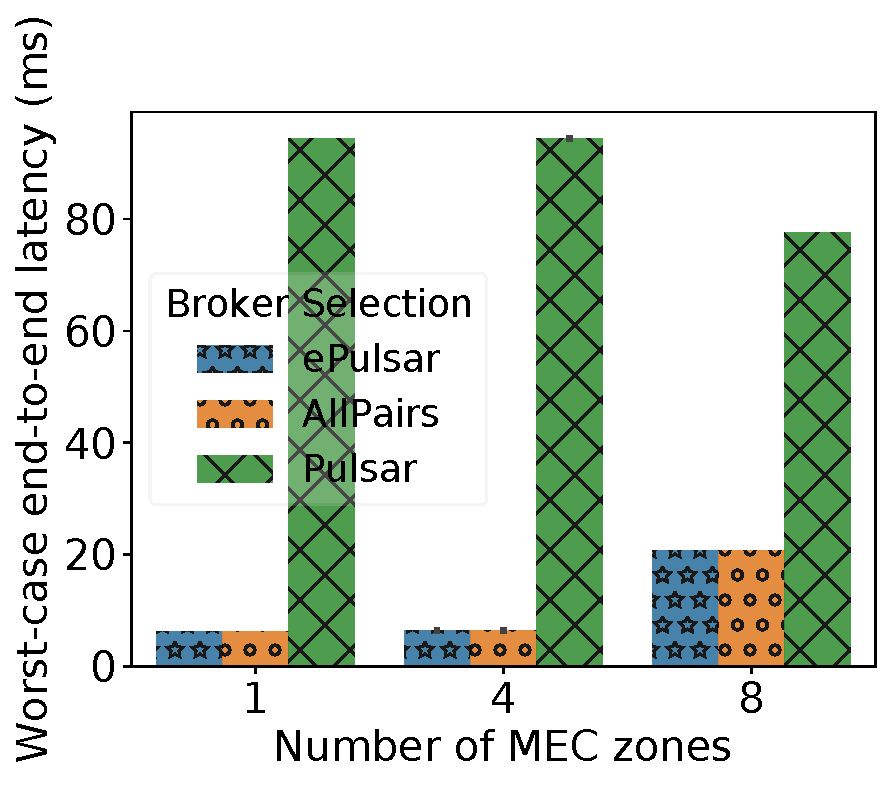
\includegraphics[width=\columnwidth]{figures/epulsar/evals/latency.pdf}
    \caption{Worst-case E2E latency}
    \label{fig:brokersel_uav_latency}
\end{subfigure}
\begin{subfigure}{.45\columnwidth}
  \centering
    \includegraphics[width=\columnwidth]{figures/epulsar/evals/violation_ratio.pdf}
    \caption{Violation Ratio.}
    \label{fig:brokersel_uav_viol}
\end{subfigure}
\caption{Analysis of broker selection policy for UAV swarm application scenario.}
\label{fig:broker_sel_uav}
\end{figure}
\cref{fig:brokersel_uav_latency,fig:brokersel_uav_viol} show the worst-case E2E latency and violation ratio over all producer-consumer pairs. Since \epulsar{} performs latency-aware broker selection, the worst-case latency remains under the threshold, resulting in no violations even when the number of MEC zones is increased. 
The results in this subsection validate the first hypothesis that the incorporation of network coordinates information in the broker selection policy improves the satisfaction of end-to-end message delivery latency constraint. Furthermore, the comparison with the AllPairs policy shows that the aggregation of clients' network coordinates as centroids does not result in poor broker selection with respect to meeting E2E latency constraints.

\subsection{Evaluation of Distributed Monitoring}
We evaluate the savings in monitoring traffic by aggregating per-topic client NCs at the serving broker before reporting them to the Metrics Store. This traffic is sent continuously through the WAN and impacts the scalability of the system, hence we consider aggregate monitoring traffic rate as the metric-of-interest. We focus our evaluation on a single broker hosting topics with multiple clients - as the behavior is independent of other brokers. We vary the number of topics hosted on the broker and the number of clients connected to each topic.
\begin{figure}[ht]
% Taken from exp ID ZKDELAY_2021-01-18-00-43-28
  \centering
  \includegraphics[width=0.9\linewidth]{figures/epulsar/evals/zk_traffic_rate__.pdf}  
  \caption{Monitoring traffic rate under varying number of topics and clients per topic. \epulsar's NC aggregation results in considerable savings over naive AllPairs.}
    \label{fig:zk_traffic_rate}
\end{figure}

\cref{fig:zk_traffic_rate} shows the data rate of monitoring traffic sent to the Metrics Store. An increasing number of topics results in higher data rate. The rate of increase is higher without centroid aggregation (AllPairs policy) and also with more clients per topic. \epulsar's aggregation, however, causes data rate to be independent of the number of clients - since a constant amount of data is sent to the Metrics Store per topic. These results validate the second hypothesis that aggregating clients' network coordinates as centroids results in reducing the monitoring overhead.

\subsection{End-to-End Evaluation}
In this section, we evaluate \epulsar's ability to respect E2E latency constraints of the exemplar UAV Swarm application, and validate the third hypothesis. The metric we use for the evaluation is E2E message delivery latency -- i.e., the elapsed time between a client publishing a message to a topic and the receipt of the published message by all the clients subscribing to that topic.

\begin{figure*}[!t]
    \centering
    \includegraphics[width=0.7\textwidth]{figures/epulsar/evals/e2e_delays_swarm_combined.pdf}
    \caption{E2E latencies experienced by the 8 independent drone swarms for their respective representative topic over time. Latency violations (transient spikes) are observed when a swarm moves from one MEC zone to another.  For a brief period, the latency remains higher than the threshold due to network traversal through the city-level switch. \epulsar's topic migration brings the latency back under the threshold.}
    \label{fig:e2e_drone_swarm_aggr}
\end{figure*}

We consider the infrastructure topology described in \cref{sec:epulsar_eval_scenario} with 4 MEC zones and emulate it using Containernet. We emulate each UAV swarm as an independent container where the mobility of all the members of the swarm are identical. In the emulated network topology, each zone consists of a network switch to which the broker and the Edge Gateway connect. We create a link between the swarm's container and the switch corresponding to the swarm's current MEC zone. When a swarm moves into a new zone, the link to the previous zone's switch is removed and a link to the new zone's switch is created. We emulate 8 independent swarms, each with 8 UAVs, following the Random Waypoint mobility model in the city at a relatively high speed of 50 meters/sec\footnote{We use such a high speed to trigger several mobility-driven topic migrations during the experiment.}. Both leader and followers generate 200 msgs/sec each of size 1 KB \cite{yang2018telecom}. We perform this experiment for 10 minutes.
\par We show the E2E latency of a single representative topic from each swarm in \cref{fig:e2e_drone_swarm_aggr}\footnote{To avoid cluttering the figure, we do not show all the topics of each swarm since their behavior is identical.}.
For each swarm. the E2E latency remains under the latency threshold  (40 ms) for most of the experiment duration. Transient violations of latency threshold occur when a swarm moves into a different MEC zone than the one currently hosting the swarm's topics. \epulsar{}'s monitoring module detects such violations and triggers migration of the swarm's topics to the broker at the new MEC zone, after which the E2E latency returns back under the latency threshold.

\section{Conclusion}
\label{sec:epulsar_conclusion}
    %\chapter{\oneedge{}: Application orchestration over geo-distributed Edge infrastructure}
\label{sec:oneedge}

\section{Introduction}

\section{Basics of Application Orchestration in Edge Computing}

In this section, we will set the stage for the discussion of how \oneedge{} leverages the mechanisms proposed in this dissertation to implement control-plane policies for application orchestration. We first present the application model that \oneedge{} supports, the application requirements for which control-plane policies need to be designed, and the challenges faced by in an Edge setting due to the dynamism in workload.

\subsection{Application Model}
\label{sec:oneedge_app_model}
Situation-awareness applications process data incoming from sensors through a series of functions, each extracting out certain information from the input data or performing a certain operation. This can be naturally modeled as a Data Flow Graph (DFG) \cite{dfg}. Each node in a DFG represents a processing function and each directed edge represents a data dependency between the upstream and downstream node. In \oneedge{}, we assume a special case of the more general DFG model, which is a pipeline of functions. As shown in \cref{fig:app_pipeline}, each DFG node, or application component, is an independent actor, and is represented by a level. Level 0 is assigned to the most downstream component, and the level number increases as we go upstream toward the client. Each component reads from a queue of input events which is populated by the upstream component and sends output events to the downstream component. An application component is also able to send events to an upstream component (including the client).

\begin{figure}[ht]
\centering
\begin{subfigure}{.48\columnwidth}
  \centering
    \includegraphics[width=\columnwidth]{figures/oneedge/app_pipeline.pdf}
    \caption{Application Pipeline.}
    \label{fig:app_pipeline}
\end{subfigure}
\begin{subfigure}{.48\columnwidth}
  \centering
    \includegraphics[width=\columnwidth]{figures/oneedge/pipeline_tree.pdf}
    \caption{Actual deployment of a pipeline-based application model resembles a forest with multiple trees.}
    \label{fig:pipeline_tree}
\end{subfigure}
\caption{Description of the application model.}
\label{fig:app_model}
\end{figure}

Although applications are modeled and specified as a linear pipeline, upon deployment for multiple clients, world, the set of application components and the data dependencies among them resemble a forest, as shown in \cref{fig:pipeline_tree}. This is because in order to serve many geo-distributed clients, the same application component needs to have several instances deployed in network proximity of clients so that communication latency to the application instance can be minimized and real-time response made possible. However, not all pipeline components have stringent latency requirements, and thus can serve multiple clients. Each tree in the forest has the most downstream application component (with level 0) as the root node and clients as leaf nodes. Each root-to-leaf path in a tree is a complete application pipeline, and we call each such path except the leaf node an \textit{application instance}. An application component that serves more than one upstream components is essentially processing information gathered from multiple clients, and therefore is able to enable state sharing among clients. However, even for applications that don't share state among clients in their logic, sharing one or more components in the application pipeline among multiple clients can be beneficial. This is because the memory footprint of running multiple independent application components is higher than sharing an application component to serve the same number of clients \todo{quantify?}.

\begin{figure}[ht]
\centering
\includegraphics[width=0.8\columnwidth]{figures/oneedge/collaborative_driving_app.pdf}
\caption{The collaborative driving assistance application modeled as a pipeline of components.}
\label{fig:collab_driving_pipeline}
\end{figure}

\par For example, the Collaborative Driving Assistance application can be modeled as a pipeline of application components as shown in \cref{fig:collab_driving_pipeline}. The Client component performs object detection on an input LiDAR sensor stream to generate a list of objects that it can see in its immediate field of view. The Sub-Regional View component aggregates the individual views from multiple vehicles that are in close spatial proximity of one another to create a composite view. This composite view is fed back to the vehicles so that they can improve their lane control and collision avoidance decisions. The output of Sub-Regional View components is processed by the Regional View component to perform higher-level analyses across a larger geographical area.

\begin{comment}
\subsubsection{Programming Model}
\begin{table}
\caption{Programming model API:  communication primitives.}
\label{table:comm_api}
\centering
\resizebox{0.95\textwidth}{!}{%
\begin{tabular}{|c|c|}
\hline
\textbf{Interface} & \textbf{Description} \\ \hline
\begin{tabular}{@{}c@{}} void send\_up (message m, edgeId o) \end{tabular} & \begin{tabular}{@{}c@{}} Sends a message asynchronously from a node \\ to the downstream node connected through edge \textit{o}. \end{tabular} \\ \hline
\begin{tabular}{@{}c@{}} void send\_down (message m, edgeId i,\\ \textbf{optional } nodeId n) \end{tabular} & \begin{tabular}{@{}c@{}}Sends a message asynchronously to all upstream \\nodes connected through edge \textit{i}.  Optionally it can \\ choose to only contact  one of the upstream nodes \textit{n}. \end{tabular} \\ \hline
\begin{tabular}{@{}c@{}} void send\_to (message m, \\nodeId destination) \end{tabular} & \begin{tabular}{@{}c@{}}Sends a message to a specific destination node.
\end{tabular} \\ \hline
\begin{tabular}{@{}c@{}} void send\_to\_partion\_clients (message m, \\partitionId id) \end{tabular} & \begin{tabular}{@{}c@{}}Sends a message to all the clients in a logical partition.
\end{tabular} \\ \hline
\end{tabular}
}
\end{table}
\end{comment}

\subsection{Control-Plane Policies for Application Orchestration}
Effective orchestration of situation-awareness applications on Edge infrastructure requires two main decisions that need to be taken by the control-plane. These two decisions are (i) mapping clients to application instances, and (ii) deploying and managing resources for application instances on Edge sites.

\subsubsection{Mapping Clients to Application Instances}
\newcommand{\clientset}{\mathcal{C}}
\newcommand{\instanceset}{\mathcal{I}}
\newcommand{\resourceset}{\mathcal{R}}

We now formally describe the decision concerning mapping clients to application instances for a specific application. Let $\clientset$ denote the set of clients for the given application and $\instanceset$ denote the set of running instances of all the components of this application. As mentioned before, each application component in $\instanceset$ as well as each client in $\clientset$ has an associated level, which indicates the stage number in the pipelined application model. The mapping of clients and upstream application components to downstream components is defined by a function $\mathcal{M}$, defined in \cref{eq:mapping_domains_eqns} and \cref{eq:mapping_eqn}.
\begin{equation}
\label{eq:mapping_domains_eqns}
\mathcal{M} : \left( \clientset \cup \instanceset \right) \times Z^+ \rightarrow \instanceset
\end{equation}

\begin{equation}
\label{eq:mapping_eqn}
\mathcal{M} \left( c, l \right) = \text{App Component of level }l \text{ serving }c
\end{equation}
The control-plane needs to compute such a mapping so as the ensure that the application requirements discussed in \cref{sec:oneedge_app_reqs} are satisfied.

\subsubsection{Deployment of Application Instances on Edge Sites}
Each application instance, comprising of all the components in the application's pipelined model, need to be deployed on a compute resource. The placement of application components ($\instanceset$) on the set of compute resources ($\resourceset$) can be represented by the function $\mathcal{P}$, as described in \cref{eq:placement_domain_eqn} and \cref{eq:placement_eqn}.

\begin{equation}
\label{eq:placement_domain_eqn}
\mathcal{P} : \instanceset \rightarrow \resourceset
\end{equation}

\begin{equation}
\label{eq:placement_eqn}
\mathcal{P} \left( a \right) = \text{Compute resource hosting }a
\end{equation}
The placement of application components is computed in a manner that meets the end-to-end latency requirements of the application, as described in \label{sec:oneedge_app_reqs}.

\subsection{Application Requirements}
\label{sec:oneedge_app_reqs}
We now discuss the requirements that \oneedge{} allows application developers to specify which allow the application
\begin{figure}
	\centering
	\includegraphics[width=0.95\textwidth]{figures/oneedge/pipeline_latency.pdf}
    \caption{
    A generic pipeline that explains the different components of the tolerable latency staleness. $S_{(i-1,i)}$ is the acceptable latency starting at the output of the client to the input of the node $i$. It is composed of both computational latency $C_j$ and transmission latency $T_{j-1,j}$.}
	\label{fig:pipeline_lat}
\end{figure}

\subsubsection{End-to-End Processing Latency}
Application developers are able to specify the end-to-end processing latency for each component in the application pipeline model. End-to-End processing latency for an application component is the time elapsed between when a specific data-item/event is generated by the client to when it is processed by the application component. This includes the network transmission latency and processing time of all the upstream components. The end-to-end latency constraint for each application component should be satisfied for each client of the given application. The end-to-end latency for client $c$ at application component with level $l$ is defined in \cref{eq:e2e_proc_latency}, which is calculated recursively using the value for the upstream component with level $l+1$. The base case is when the level $l$ equals the level corresponding to the client itself, in which case, the end-to-end latency is equal to the processing latency on the client.
\begin{equation}
\label{eq:e2e_proc_latency}
E2E \left( c, l \right) = E2E \left(c , l+1 \right) + proc \left( \mathcal{M} \left( c, l \right) \right) + net \left(  \mathcal{M} \left( c, l+1 \right) , \mathcal{M} \left( c, l \right) \right)
\end{equation}

\subsubsection{Spatial Affinity}
Several situation-awareness applications such as the collaborative driving assistance application (\cref{fig:collab_driving_pipeline}) consist of components that are tied to a specific geographical area, and are meant to serve clients located in that geographical area only. This is meant to enable information sharing between clients that are in close spatial proximity to one another. We denote the geographical area served by an application component as its \textit{spatial context}. The partitioning of the geographical space into spatial contexts is application-specific. More precisely, the application developer would specify a function $\mathcal{S}$ that maps a geographical location $\left( x , y \right)$ to a unique spatial context $s_z$ (identified by a positive integer $z$) (\cref{eq:spatial_context}).

\begin{equation}
\label{eq:spatial_context}
   \mathcal{S}: X \times Y \rightarrow \{ s_0, s_1, \cdots \}
\end{equation}
\begin{equation}
   X = \{x \in \mathbb{R}~|~-\pi < x < \pi\}
\end{equation}
\begin{equation}
   Y = \{y \in \mathbb{R}~|~\dfrac{-\pi}{2} < y < \dfrac{\pi}{2}\}
\end{equation}

For an application component of level $l$ that needs to facilitate inter-client information sharing, the control-plane assigns each spatial context $s_z$ with an application component and map all clients located within that spatial context to that instance. Multiple spatial contexts can also be mapped to the same application instance. However, the main requirement is that all clients within given spatial context should be served by the same application instance so that they can effectively share state with other clients in the same spatial context. The quality of this client-application-instance mapping is quantified using the Spatial Alignment metric, as shown in \cref{eq:spatial_alignment}. The Spatial Alignment metric is defined for each spatial context $s_z$ that is served by the application component instance $a$ at level $l$.  Ideally, the spatial alignment metric should be equal to 1 for all spatial contexts.
\begin{equation}
\label{eq:spatial_alignment}
SA \left( a \right) = \dfrac{|\{ c \in \clientset : c.loc \in s_z   \mathcal{M} \left( c, l\right) = a \}|}{|\{ c \in \clientset : c.loc \in s_z \}|}
\end{equation}
\todo{Can we connect application instance $a$ with $s_z$?}

\subsection{Workload Dynamism}

\subsubsection{Client Mobility}
Typical situation-awareness applications have clients that are inherently mobile, for example, vehicles, pedestrians, UAVs, etc. The mobility of clients creates two main challenges. For applications involving inter-client information sharing, the mapping of a client to an instance of a given component is based on the spatial context of that component's instance and the location of the client. Due to client mobility, the client's location might change so much that it exits the spatial context of the current application component instance, and thus is not able to coordinate with the correct subset of other clients that are in its physical proximity. This requires that the client be migrated to the application component instance that has the correct spatial context which corresponds to the current location of the client. Secondly, client mobility can result in a change in the network routing and hence communication latency to and from the application instance. This change in communication latency affects the end-to-end processing latency for that client's data by the current application instance. This necessitates that the client be migrated to an application instance that can satisfy the end-to-end latency requirements.

\subsubsection{Changes in Processing Requirements of Applications}
The frequency of events generated by different application components in an application pipeline changes over time. This is either due to the mobility of clients which changes the properties of the environment sensed by the clients. For instance, in the Collaborative Driving Assistance application, the number of neighboring vehicles output by the Detection component (in the client) is a function of the density of neighboring traffic, which changes with time as the ego vehicle moves. The change in processing requirements of applications can also happen for static sensors, such as CCTV cameras, when the environment they are sensing undergoes changes. For instance, in the \todo{} application, the frequency of events generated by the \todo{} component depends on the number of cars in the field-of-view of a camera, which changes over time.

\section{Architectural Components of \oneedge{}}
Now we present the system architecture of \oneedge{}, covering the design choices and deployment characteristics of each component of the system. We will first provide a high-level overview of the system, with an emphasis on describing how \oneedge{} operates and the typical operations of each component. Then we will discuss the functions of each component in more detail.

\subsection{High-level System Architecture}
\begin{figure*}[t]
\centering
\includegraphics[width=0.85\columnwidth]{figures/oneedge/onefog_overview.png}
\caption{\oneedge{}'s System Architecture. A central controller (left blow-up) coordinates with all the Edge sites (right blow-up).}
\label{fig:system_arch}
\vspace{-2mm}
\end{figure*}
\cref{fig:system_arch} shows the high-level system architecture of \oneedge{}, which comprises of two main top-level entities: the \emph{Edge Site} and \emph{Controller}. An Edge Site is an independent entity with compute and storage resources that is able to run instances of application components and serve clients. The Controller is a logically-centralized entity which is responsible for the scheduling and deployment of applications over multiple Edge Sites. 

\todo{Autonomous updates to resource allocation on sites.}

\par Application clients run the client component of the application pipeline and are served by an application instance running on one or more Edge sites. To connect to a suitable application instance, clients send deployment requests to the geographically closest Edge site (determined by using a standard discovery service\cite{citation_21_in_oneedge_paper}). If the nature of the application is such that it does not require information from other clients and the Edge site receiving the deployment request has enough resources, then the application is deployed entirely on that Edge site. Otherwise, the deployment request is sent to the Controller, which computes the application scheduling decision and launches application components across potentially multiple Edge sites.
\todo{Add that the Monitoring Subsystem issues reconfiguration requests that need to be serviced either by the controller or the site }

\subsection{Client Library}

\subsection{Components on Edge Site}
An Edge site consists of four main components, as shown in the right blow-up in \cref{fig:system_arch} - the Site Agent, Container Runtime, Container Agent and the Monitoring Subsystem. 
\subsubsection{Site Agent}
The Site Agent component is responsible for managing the resources on the site, along with the application component instances running on the site. It receives requests from clients for connection to an application instances, and deploys instances of the application pipeline's components in response. It also interfaces with the central Controller for the centralized scheduling of applications on that Edge site. Specifically, the Site Agent provides periodic updates to the Controller about the allocation state of application component instances running on the site. In addition, it also receives commands from the Controller to deploy application component instances. The Site Manager is also responsible for lifecycle management of the running application component instances, wherein, it updates the resource allocation of these instances based on requests triggered by the Monitoring Subsystem, which will be discussed in more detail in \cref{sec:oneedge_monitoring}.
\subsubsection{Container Runtime}
The Container Runtime is the software platform upon which the various application component instances run as containers. The container runtime provides primitives for launching containers based on an application-specific image, allocation a specific amount of compute and memory resources to containers to ensure predictable performance and isolation, access to a filesystem for storing ephemeral state and communication with other entities in the system. 
\subsubsection{Container Agent}
The Container Agent is a software agent which is deployed alongside the application logic within each application component instance's container. It acts as the interface of the application logic for that specific application component with the rest of the components and the outside world. It does so by implementing the various interfaces provided to the application developer. The container agent facilitates communication between various application instances by allowing upstream and downstream components to send messages to each other, as well as trigger callback functions in the application logic upon message arrival. Furthermore, it also serves as a part of the monitoring subsystem, whereby it collects metrics related to the execution of the application component and forwards them for further processing.
\subsubsection{Monitoring Subsystem}
\todo{Add text for the Monitoring Subsystem.}

\subsection{Controller}
The Controller component is responsible for application scheduling and management at a global-scale across Edge sites. It receives requests for application deployment and reconfiguration from clients and the monitoring subsystem respectively. These requests are processed by the Scheduler, which turns these requests into a transaction (set of actions) to be executed on one or more Edge sites. The transaction is then added to the pool of pending transactions waiting to be executed on the respective Edge sites. The Transaction Executor picks up a pending transaction and executes the actions contained in them on one or more Edge sites. We will discuss each of the components in greater detail next.
\subsubsection{Scheduler}
\label{sec:scheduler}
\begin{itemize}
\item The Scheduler picks up one request at a time from the Controller's request queue and computes a scheduling decision for the request. The scheduling decision is computed by executing the placement algorithm (\cref{todo}) for mapping the requesting client to a suitable application instance that can satisfy the end-to-end latency and spatial affinity requirements. If no such application instance exists, a new instance is instantiated and suitable Edge sites for hosting the application components are selected.
\item In the case of a reconfiguration request for updating allocation of an application instance, the scheduler computes the final resource allocation for the components of that application instance.
\item The Scheduler reads the Aggregate Resource State to check the current available resource capacity on each Edge site, and updates the state with changes to the resource allocation. Hence, the Aggregate State is \textit{optimistically} updated even before the scheduling decision has actually been applied on the specific Edge sites. By doing so, the process of compute application scheduling decisions is decoupled from the actual enforcement of those decisions on the Edge sites.
\item The scheduling decision is in the form of a Transaction, which is a collection of the actions that need to be taken to execute the scheduling decision. The constituent actions of a transaction need to executed on one or more Edge sites. 
\end{itemize}

\begin{minted}{yaml}
-   app_id: 
    txn_id: 
    actions: 
        -   site_id: 
            site_actions:
                -   level: 
                    type: DEPLOY
                    resources: 
                        cpu:
                        memory: 
                -   level: 
                    type: MODIFY_ALLOC
                    resources:
                        cpu: 
                        memory:
\end{minted}

\subsubsection{Aggregate State}
\label{sec:aggr_state}
\begin{itemize}
\item As described in \cref{sec:scheduler}, the Aggregate State is used by the Scheduler to make application scheduling decisions. For subsequent requests' processing to be aware of the decisions made for the current request, the Aggregate State is updated with the current request's decisions. 
\item The Aggregate State maintains an optimistic version of the resource allocation state, assuming that all the scheduling decisions taken by the Scheduler will successfully get enforced on the Edge sites.
\item However, since Site Agents have the autonomy to make resource allocation changes without coordinating with the Controller, scheduling decisions from the Controller could be rejected by the Site Agent, in which case the corresponding Transaction would be aborted.
\item The abortion of a transaction would result in rolling back the Aggregate State to a state before the aborted transaction's processing was begun by the Scheduler.
\item In addition to having applied updates that have not yet been successfully applied on Edge sites, the Aggregate State is also eventually consistent with the ground-truth resource allocation which is maintained by the Site Agents. Since Site Agents are able to update allocation state of the site without coordinating with the Controller, the Controller's Aggregate State does not see those autonomous updates until the state is synchronized with the Edge site, which is done periodically.
\end{itemize}
\subsubsection{Pending Transactions Pool}
The Transactions generated by the Scheduler are buffered in the Pending Transactions Pool so that their constituent actions can be enforced on the Edge sites. However, transactions can only be executed in the order in which they were processed by the Scheduler. The relationship between transactions that defines the order in which they are executed can be denoted as $T_i \leftarrow T_j$, in this case denoting that the transaction $T_i$ can be executed only when $T_j$ is executed. In other words, the Aggregate State output by $T_j$ was used as input for $T_i$. The following conditions have to be met for $T_i \leftarrow T_j$ to be true:
\begin{itemize}
\item $T_j$ was generated by the Scheduler before $T_i$.
\item The set of Edge sites affected by $T_i$ and $T_j$ overlap.
\end{itemize}

\subsubsection{Transaction Executor}
\begin{itemize}
\item 
\end{itemize}
\section{Spatial-Affinity-aware Application Scheduling using Dynamic Spatial Context Management}
\begin{itemize}
\item An application can have multiple components that are tied to their specific spatial contexts. The constraint imposed by \oneedge{} is that the spatial context of an upstream component should be completely present inside the spatial context of the downstream component. This is done to ensure that the each instance of the downstream component has only one parent instance. 

\end{itemize}
\subsection{Flexible Partitioning of Geographical Space}
\begin{itemize}
\item For each of the application components that are spatially constrained, the control-plane maintains a KD-Tree based spatial partitioning, as discussed in \cref{sec:spatial_ctx_mgmt}. 
\end{itemize}

\subsection{Control-Plane Policy for Spatial-Affinity-aware Application Scheduling}

\section{Latency-aware Application Scheduling using Network Proximity Estimation}

\subsection{Deployment of Network Coordinate Agents}

\subsection{Estimating End-to-End Processing Latency}

\subsection{Control-Plane Policy for Latency-aware Application Scheduling}

\section{Distributed Monitoring in \oneedge{}}
\begin{itemize}
\item The goal of monitoring in \oneedge{} is to detect violations of performance SLO, which in this case is end-to-end processing latency.
\item The end-to-end processing latency constraint is specified for one or more components of the application pipeline. The end-processing-latency at a certain component is the sum of the processing and communication latencies of the application pipeline instance right from the client up to (and including) the given component.
\item The objective of \oneedge{} is to detect when any constraint on end-to-end processing latency in an application instance is violated, and then trigger the appropriate reconfiguration action to alleviate that violation.
\item Another crucial objective of monitoring in \oneedge{} is to identify the root-cause of the end-to-end processing latency violation, which is used to determine the appropriate reconfiguration action that can alleviate the violation.
\end{itemize}

\subsection{Metrics}
Each application component instance registers two metrics with the monitoring subsystem. 
\begin{enumerate}
\item The network latency between the given application component instance and its immediate downstream component (also known as \textit{parent}). 
\todo{Add parent ping process in ContainerAgent description}
\begin{minted}{yaml}
-   entity_id : <ID of application component instance>
    level : <level in application pipeline of component>
    app_unit: <ID of root component instance in application tree>
    metric: "net_latency"
    parent: <ID of parent component instance>
\end{minted}
\item Processing latency at the given application component instance.
\begin{minted}{yaml}
-   entity_id : <ID of application component instance>
    level : <level in application pipeline of component>
    app_unit: <ID of root component instance in application tree>
    metric: "proc_latency"
    parent: <ID of parent component instance>
\end{minted}
\todo{Do we need parent field in $proc\_latency?$}
\end{enumerate}

\subsection{Violation Detection Policy}
\begin{algorithm}
\caption{$End-to-End Processing Latency Violation Detection policy$}
\begin{algorithmic}
\Require ID of root worker $ID_{root}$ ($A_{00}$ in \cref{fig:pipeline_example}).
\Require Application abstract $APP$
\State $MD \gets \text{Fetch metrics where AppUnit == }A_{00}$
\State $C \gets \{ m.entity\_id \forall m \in MD : m.level == APP.num\_levels-1 \}$
\State $entities \gets \{\}$ \Comment{Dictionary to hold proc and net latencies for each worker}
\For{$m \in MD$}
    \If{$m \notin entities$}
        \State $entities[m.entity\_id] \gets \{\}$
    \EndIf
    \State $entities[m.entity\_id][m.metric] \gets m$ 
\EndFor

\State $violators \gets \{\}$
\For{$c \in clients$}
    \State $e \gets c$  
    \State $e2e \gets 0$
    \State $level \gets APP.num\_levels-1$
    \While{$level \geq 0$} \Comment{Iterating over all levels of app pipeline}
        \State $e2e += entities[e][proc\_latency].val + entities[e][net\_latency].val$
        \If{$e2e \geq APP.e2e\_threshold[level]$}
            \State $violators \gets violators \cup \{ \left( c, level \right) \}$
        \EndIf
        \State $level -= 1$
        \State $e \gets entities[e][net\_latency].parent$
    \EndWhile
\EndFor
\Return $violators$
\end{algorithmic}
\end{algorithm}

\subsection{Violation Root-Cause Analysis Policy}

\section{Implementation}

\section{Evaluations}

\section{Conclusion}
    %\chapter{FogStore}

Situation-awareness applications maintain state, that guides the action of the application in the future. Application state consists of recently generated events (such as a vehicle detection) and location-tagged data-items (such as the state of a traffic light). Hence, system support primitives for {\it saving and retrieving events} that constitute the application state are critical in a service platform meant for geo-distributed applications. Contemporary stream processing platforms like Foglets \cite{foglets}, Apache Flink \cite{flink} and Samza \cite{samza} provide primitives for accessing and modifying the application state. Quite often, multiple application components on different edge nodes may want to share the application state -- e.g.,  situation-awareness applications may have multiple processes working on events pertaining to the same geographical area; this would require moving the state out of memory into an out-of-core external store \cite{sharedstateflink} - a design choice that is also supported by Apache Flink. Keeping such application state information on Cloud-based data stores would defeat the purpose of placing the application components in geo-distributed fog/edge nodes since saving/retrieving state is in the critical path of the application execution and should incur as little latency as possible. Hence, the application state needs to be stored in a geo-distributed manner as well \cite{confais2017performance}, leveraging the same edge nodes as those used for placing the computational components. 
\par Situation-awareness applications have stringent timing requirements on the sense-process-actuate control loop, which involves accessing application state in the critical path. To ensure that the application's control loop can operate at the desired speed, access to application state needs to be possible with low latency. Situation-awareness applications require strong consistency guarantees on the application state \cite{consistentstreaming}. In fact, researchers at Google observe that coping with eventual consistency in the application layer requires significant development time and often leads to complicated and error-prone mechanisms \cite{f1}. Hence strong consistency should be provided by the datastore layer itself. Furthermore, the application state should remain available in spite of failures of data store nodes.
\par Cloud-based data stores such as Cassandra, DynamoDB, etc. have a performant data-plane which offers low latency of data access. They also offer strong consistency guarantees along with fault-tolerance. However, Edge infrastructure poses peculiar challenges which are not present in Cloud datacenters, for which these systems are designed. Firstly, the network topology of the Edge infrastructure is highly heterogeneous, and low latency data access is only possible if the data replicas are located close to the client. Ensuring strong query consistency demands that the data replicas on which query is executed are located in proximity to the client. However, Edge infrastructure is more susceptible to geographically correlated failure, which increases the probability of making multiple replicas of a given data-item unavailable. Hence, latency, consistency and failure tolerance are conflicting objectives at the Edge, and the control-plane of off-the-shelf data stores do not offer a reasonable tradeoff between them. 
\par FogStore tackles the problem of providing both the conflicting but valid objectives of fault-tolerance and low-latency while satisfying consistency guarantees in geo-distributed key-value stores. The key insight about situation-awareness applications is the dependence of relevance of a certain data-item on the client's context. For instance, in the smart city domain, information related to a particular city may be relevant to clients who are in close proximity to that city. Using this context-sensitive characteristic of applications, we design a replication strategy that guarantees strong consistency for relevant data replicas and eventual consistency for the replicas intended primarily to ward off geo-correlated failures.  
%we trade-off globally consistent access to application state for low-latency and fault-tolerant access with strong consistency guarantees to clients for whom the data item is contextually relevant. 
The strategy is to place replicas close to the relevant clients (for low latency) and also in geographically distant locations (for fault-tolerance).
% and making a distinction in how consistent these replicas are kept. The replicas close to relevant users are kept strongly consistent, while those away are kept eventually consistent. 

{\it FogStore}, which embodies the design principles for achieving fault-tolerance and low-latency for strongly consistent access to application state makes the following contributions:
%The following points sum up the contributions of this paper :
\begin{itemize}
    \item Develop a notion of \textit{relevance} for situation-awareness applications, which is formalized as \textit{Context-of-Interest} (CoI) - which determines the degree of consistency at which queried state should be reported;
    \item FogStore utilizes the Dynamic Spatial Context Management mechanism to perform location-aware replica placement to ensure low latency data access along with tolerance from geographically correlated failures.
    \item FogStore utilizes the Dynamic Spatial Context Management mechanism to perform quorum selection that guarantees strongly consistent operations for \emph{relevant} data.
\end{itemize}
The roadmap of this chapter is as follows. \cref{sec:background} provides a background of the motivating application scenario and the basic concepts of a key-value store. It also discusses in detail the requirements of situation-awareness applications and the challenges of meeting those requirements in an Edge setting. \cref{sec:fogstore_arch} presents the architecture of FogStore. \cref{sec:replica_placement} describes how FogStore leverages the Dynamic Spatial Context Management mechanism to perform replica placement to ensure low-latency data access along with tolerance from geographically correlated failures. \cref{sec:consistency_tuning} describes how FogStore uses the same mechanism to perform quorum selection to ensure high consistency data access for \textit{relevant} data items. \cref{sec:evals} presents results of experimental evaluation of FogStore and \cref{sec:conclusion} concludes the chapter.

\section{Background}
\label{sec:background}

\subsection{Motivating Application Scenario}
\label{sec:fogstore_application}
To highlight the necessity of a system like FogStore, we present a motivating use-case that poses strict latency and staleness requirements on the data-store. Consider a distributed camera network that may be deployed on urban roadways, feeding real-time video streams for multi-camera tracking of suspicious vehicles. 

\begin{figure}
\includegraphics[width=\columnwidth]{figures/fogstore/vehicleTrackingFlow.png}
\caption{Schematic of multi-camera tracking of suspicious vehicles. The numbered arrows suggest the temporal order of flow of information.}
\label{fig:usecase-schematic}
\end{figure}

\par The application can be logically partitioned into components, as per the MobileFog programming model \cite{mobilefog}, each performing a specific function and having well-defined input-output characteristics. A schematic of the application is presented in Figure \ref{fig:usecase-schematic}. Upon detection of a vehicle in a video frame, the application extracts the identity of the vehicle by reading the license plate to get the unique identifier of the vehicle. It then inserts the detection of that vehicle along with location and time into the set of detections. The application also maintains the complete trajectory information of the vehicle, in that, for each detection of a vehicle, it saves the location and time when the car was detected before that. To achieve this, for each detection the application retrieves the set of previous detections that took place within 5 KM and 10 minutes from the current detection. It looks for the most recent detection from them and adds the identifier of that detection to the current detection's $prevDetection$ field.

\begin{algorithm}
\caption{Vehicle tracking algorithm}\label{usecasealgo}
\begin{algorithmic}[1]
\Procedure{onDetectVehicle}{V, X, Y, T}
%\State $K \gets \text{INSERT INTO vehicle\_detections} $
\State $K \gets \text{INSERT INTO vehicle\_detections} \left(V, X, Y, T \right)$
\State $prevDets \gets \text{SELECT * FROM vehicle\_detections} \newline \text{WHERE } \left( x,y \right) \text{within 5 km } \& t \text{ WITHIN 10 min ORDER BY t }$
\State $prevDet \gets k.V : k \text{ has most recent time in } prevDets$
\State $\text{UPDATE K in vehicle\_detections SET K.prevDet = prevDet}$
\EndProcedure
\end{algorithmic}
\end{algorithm}
\par It is evident from the schematic that access to application state lies in the critical path of application execution, hence making correct execution of the application contingent on fast access to state. For instance, if the insert of a vehicle detection is slow, the vehicle may be detected by an adjoining camera and not mark the former detection as the previous one - hence missing that detection from the trajectory. It is worth noting that the presented application has a dependence on contextually relevant events, specifically previous detections within a 5 km radius and at a maximum of 10 minutes before the current detection. Events that don't fall under this space-time filter may be past detections of the car but are typically not relevant for generating a fine-grained trajectory. Furthermore, retrieving the entire set of previous detections of the particular car and searching for the most recent detection could be slow. 

\subsection{Interface offered by a Key-Value Store}
\subsubsection{Data Model}
The data-model of FogStore follows a key-value pair model, wherein keys are strings and values can be elementary data-types such as strings, integers or floating point numbers, or a dictionary of key-value pairs themselves. Following are the types of key-value pairs that data-items of typical applications contain.
\begin{itemize}
\item Each data item needs to possess spatial information, that is, location in terms of latitude-longitude. This field denotes the location of the event or entity that the data-item is about.
\item Data-items, especially those that pertain to events that happened at a certain point of time, contain a timestamp field.
\item Data-items are allowed to contain key-value pairs specific to the application's logic, such as vehicle identifier in the case of a multi-camera vehicle tracking application.
\item It is up to the developer to specify which keys of a set of data-items constitute the primary key, which will be used to uniquely identify data-items for queries.
\end{itemize}

\begin{lstlisting}[caption={A sample data-item that captures a spatio-temporal event in the vehicle-tracking application's detection set. The field storing Vehicle ID forms the key that will be used to retrieve detections of a particular vehicle.},captionpos=b,label={lst:listing1},language=Json]
{
  "vehicle_id": "A54 3527",
  "location": {
    "latitude": "33.42553",
    "longitude": "-84.74456",
  },
  "timestamp": "1520123197"
}
\end{lstlisting}

\subsubsection{Types of Query Supported}
FogStore supports the following types of queries.
\begin{itemize}
\item \textbf{Insert/Delete data-items. } FogStore allows applications to insert data-items into the store by providing the key-value pairs that make up the data-item, including the primary key. For deleting a data-item the application can simply use the primary key.
\item \textbf{Update data-items. } FogStore allows applications to update an existing data-item by providing the primary key of the data-item and the new set of key-value pairs. If the key exists the value will be updated, otherwise a new key-value pair will be added to the data-item.
\item \textbf{Selecting data-items. } Applications can fetch data items whose key-value pairs match a certain predicate. The predicate can either be an exact match on one or more keys or an inequality-based condition.
\end{itemize}

\subsubsection{Replication and Consistency of Data}
\label{sec:replication}
\begin{itemize}
\item Key-value pairs which belong to the same application have keys that belong to the same keyspace. 
\item Dynamo-style data stores map data to storage nodes by computing a hash-function on the key. The output range of the hash function is divided among the storage nodes such that if a key's hash falls within the partition that is mapped to a particular storage node, then the key-value pair will be mapped to that node. 
\item Each storage node is assigned a \textit{token} on the output range of the hash function. The storage node with the smallest token that is greater than the hash value of a key is assigned as the primary replica of the key-value pair (as shown in \cref{fig:hashring_replication}). Additional replicas are chosen based on the requirements of the application (replication factor, rack-awareness, etc.) and the primary replica.
\end{itemize}

Key-value stores built on the Dynamo-style model offer fine-grained tuning options for consistency per-operation. Figure \cref{fig:hashring_replication} shows how Cassandra (a popular Dynamo-style key-value store) distributes data among the cluster nodes. The data-item’s key is hashed to determine the nodes responsible for storing it (replicas). The client making read/update requests can specify a consistency level for that specific operation, which determines the number of nodes that need to execute that operation before the client is acknowledged of its completion. For example, an update operation with consistency level of TWO would update the copy of the data-item on 2 of the replica nodes and acknowledges that the update was successful. The update is propagated to the rest of replicas in an eventual manner. The choice of this consistency level plays a crucial role in tuning the tradeoff between latency and consistency. Eventually consistent implementations use a consistency level of ONE while strong consistency implementations use consistency level of QUORUM. In a highly geo-distributed datastore, synchronizing with all replicas for every operation can be extremely slow, given that the replicas may be stored on nodes with a high network round-trip-time from the client/coordinator.

\begin{figure}
\centering
\includegraphics[width=0.7\linewidth]{figures/fogstore/basics/hashring.pdf}
\label{fig:hashring_replication}
\caption{Demonstration of write-request path for a 12-node
Cassandra cluster on keyspace with Replication Factor (RF)
= 3}
\end{figure}

\subsection{Control-plane Decisions involved in a Key-Value Store}
FogStore is a geo-distributed key-value store with data stored on multiple Edge sites. FogStore needs to make the following two control-plane decisions.
\begin{itemize}
\item \textbf{Replica Placement.} FogStore needs to determine the data store nodes that should host the replicas for a particular of data-item.
\item \textbf{Quorum Sizing. } For each query, FogStore needs to decide how many of the existing replicas of the queried data-item should be contacted before returning the result to the client. For read queries, the query coordinator node reads the data-item from Q replicas of the data-item and returns the latest version to the client, where Q denotes the quorum size selected. Similarly in the case of an insert or update query, the query coordinator returns success to the client as soon as the query has been executed on Q replicas.
\end{itemize}

\subsection{Application Requirements}
\begin{itemize}
\item \textbf{Low-Latency of Data Access. } State access is in the critical-path of typical applications. Hence, low-latency data access would allow the application instances to maintain their response-time.
\item \textbf{High Consistency. } For those data-items that have multiple readers and writers, applications require that the version of data that they read is the latest version. Reading a stale version of the data could result in errors in the application logic. Ensuring strong consistency in the application layer requires significant development time and often leads to complicated and error-prone mechanisms \cite{shute2013f1}. Hence, the data store is responsible for providing data access with strong consistency guarantee.
\item \textbf{Failure Tolerance. } Applications assume that with sufficient number of replicas of each data-items, at least one copy of a data-item will always be available for accessing in the event of failures.
\end{itemize}

\subsection{Challenges in achieving Application Requirements}
Operating a data store over a geo-distributed Edge infrastructure has a number of unique challenges arising out of the nature of the infrastructure.
\begin{itemize}
\item Network topology of the Edge infrastructure is heterogeneous, with Edge sites connected to the Internet through different peering points. This makes the latency between Edge sites heterogeneous. Hence, the data-placement strategies used in cloud-based data stores that ensure uniform load-balancing across storage nodes would result in high data-access latencies at the Edge.
\item High-consistency data read and writes require performing operations with multiple replicas of a data-item. In an Edge-based data store, where the inter-node latency distribution is heterogeneous, low-latency data access with high-consistency can only be achieved if all the replicas in the quorum are located close to the query coordinator.
\item Edge infrastructure consists of sites that often share the same network and power lines. These sites are susceptible to geographically correlated failures. Hence, placing all replicas of a data-item on nodes in proximity of each other to ensure low-latency high-consistency access would result in making that data-item more vulnerable to such failures. In such an event, all replicas of that data-item would be lost.
\item Data-items that compose the state of situation-awareness applications are generated due to activity in the physical environment. Spatial skews exist in the distribution of activity. For instance, within a city, there may be surveillance cameras deployed only in a certain portion of the city (e.g. Downtown), which would create a skew in terms of the number of events pertaining to those areas compared to rest of the city. Storing data-items on storage nodes that are located close to the location of the data-item itself would result in workload skews, which would impact query performance and increase the storage requirement on a subset of nodes. This problem is avoided in datacenter-based data stores by using consistent hashing \cite{consistent_hashing} to distribute data-items across storage nodes, but that would significantly deteriorate query latency in a geo-distributed data store.
\end{itemize}
Hence, low-latency, high-consistency and tolerance from geographically-correlated failures are conflicting objectives in an edge infrastructure setting.

\section{Architecture of FogStore}
\label{sec:fogstore_arch}
In this section, we first describe the edge-centric control-plane policies in FogStore at a high-level, that allow it to meet the application requirements. Then we discuss the functionalities of the system components in FogStore.

\subsection{Edge-centric Control-plane Policies}
FogStore's control-plane policies for replica placement and quorum sizing aim at simultaneously providing the application requirements of low-latency, high-consistency and tolerance from geographically-correlated failures, while dealing with the specific challenges of the Edge infrastructure. It does so by utilizing a peculiar characteristic in the data-access pattern of situation-awareness applications, wherein certain data-items are of higher relevance for the application logic if they are located in the \textit{spatial context} of a given instance of the application. We call the spatial context of the application instance Context of Interest, which is explained further in the following.
\subsubsection{Context of Interest}
Situation-awareness applications have a strong notion of locality-awareness. For example, in the case of publish-subscribe systems, the publishers and subscribers are often located geographically close to each other, because the events they are concerned with pertain to the local geographical area. This property was exploited by Teranishi et al. \cite{teranishi2015scalable} with the Locality-aware publish-subscribe system. In general, geo-distributed applications possess the notion of contextual relevance, in that a given data-item is more relevant in a certain context than another. The notion of context is highly application-specific. For instance, in the use-case mentioned in \cref{sec:fogstore_application}, a vehicle detection is relevant at a higher degree in a context around the event in space and time, that is, within 5 kms from the event’s location and within 10 minutes of the event generation. This is because of the nature of the application - to build an accurate trajectory of a vehicle, the previous detection has to be in proximity to the current detection. Similarly, smart cars accessing the state of a traffic light (red/green), where the cars located in proximity to the traffic light, would require consistent access to traffic light state to prevent collisions. Clients not in the traffic light's proximity would be able to live with data that may be stale, that is, eventual consistency may be good enough for them. Often the data generated by Internet-of-Things applications are used for big-data analysis, which are offline batch processing tasks and don’t require highly consistent data. In the context of key-value stores, the notion of relevance translates to consistency and staleness as follows : all relevant items must be available in a consistent manner with minimum staleness. In other words, for a data-item $I$ all entities for whom $I$ is contextually relevant must see updates to $I$ in the same order (serializability) and with as low staleness as possible (real-timeliness).

\par We now formally define the above notion of contextual relevance. Fogstore allows the application developer to specify a generic (possibly conservative) \emph{region of relevance} (also called Context of Interest) around each data item such that operations originating from that region are executed in a strongly consistent manner. In this paper, this region of relevance is articulated as a bounding box in geographical space. The size of the CoI is configurable and application-specific. Fogstore would compare the location of a client to the location of the queried data-item and would provide a strongly consistent result only when the client's location lies within the CoI of the data-item. Clients beyond the region of relevance are typically not using the data for critical operations and hence can tolerate inconsistent/stale data to the same extent as an eventually consistent database.

\subsubsection{Two Replica Types offering Differential Consistency}
\label{sec:two_replica_types}
We would like to revisit the two fundamental requirements of situation-awareness applications:
\begin{itemize}
\item Clients sharing context with the data-item require low-latency access to strongly consistent data
\item Placement of all replicas in proximity may lead to complete data loss under geographically-correlated failures
\end{itemize}

These requirements lead us the design decision of having two classes of replicas, which is also illustrated in \cref{fig:architecture}.
\begin{enumerate}
\item \textbf{In-CoI replicas} : Placed on nodes located at low network delay from the clients, typically within/around the CoI of the data-item.  Their maximum distance from the data-item's location is determined by a parameter \emph{InCoIDist}. This parameter determines the location of InCoI (strongly consistent) replicas and hence has implications on the latency of query operations. These replicas are kept consistent by enforcing that all read and write quorums include a majority of these replicas. These replicas are meant to provide both low-latency and strong-consistency to users that are contextually relevant to the queried data-item.
\item \textbf{Out-CoI replicas} : The purpose of these replicas is to provide tolerance from geographically-correlated failures. They are placed on datastore nodes which are a minimum distance away from the data-item's location, a parameter called \emph{OutCoIDist}. This parameter determines the location of OutCoI replicas, and hence affects the geographical separation between InCoI and OutCoI replicas - and thereby the fault-tolerance. These replicas are kept eventually consistent by propagating updates asynchronously, and hence are never included in the read/write quorum operations originating from within the CoI. These replicas could also serve as the source of data for big-data analysis of information generated at the edge, by using tools like Kafka Connect \cite{kafkaconnect} that can use key-value stores as data sources for large-scale analytics.
\end{enumerate}

\begin{figure}[h]
\centering
\includegraphics[width=0.8\columnwidth]{figures/fogstore/architecture.pdf}
\caption{Illustration of the two types of replicas maintained by Fogstore along with the typical use-cases that both these types serve. The dotted circle around the spatio-temporal data-item denotes the Context-of-Interest for the data-item. We direct all reads/updates to that data-item originating within the CoI (represented by red crosses) to the InCoI replicas (which are shown inside the circle). The other (OutCoI) replicas are kept eventually consistent and serve the use-cases dealing with batch processing and monitoring.}
\label{fig:architecture}
\end{figure}

\par It is worth noting that the concept of differential consistency for replicas based on their context is not a novel concept proposed in this dissertation. Apache Cassandra itself provides a consistency level called LOCAL$\_$QUORUM \cite{localquorum} that makes sure that any operation selects a quorum that consists of the quorum-set of replicas on the local datacenter on which the request-handler (coordinator) node is located. This is done to avoid the high latency of inter-datacenter traversal. The updates are propagated to rest of the replicas (in other datacenters) in an eventual manner. However, this concept is easy to adopt in the context of cloud-based data-stores, which have a well-defined notion of datacenters such that the network latency across datacenters is at least an order of magnitude higher than intra-datacenter latency. Data stores deployed on densely geo-distributed Edge infrastructures cannot make use of such a concept, especially when the concept of contextual locality is based on node location and geographical distance rather than simpler properties like a datacenter identifier or IP address subnet. 

\subsubsection{Handling skews in event workload}
FogStore's replica placement policy ensures that InCoI replicas are located close to the location of the data-item, while also ensuring that the workload across data-storage nodes is balanced. It does so by incorporating a hash-based replica placement approach akin to datacenter-based data stores into the location-based policy. More concretely, among the candidate nodes that fulfil the condition of InCoI replicas being close to the data-item's location, FogStore tries to use hashing to map the replica to candidate nodes. By doing so, FogStore not only achieves location-awareness but also ensures that the workload is evenly distributed among all candidate storage nodes. This notion of proximity is tunable, and can be set to match the degree of skew in workloads.

\par Hence the major issues that the implementation of Fogstore should resolve are :
\begin{itemize}
\item Placement of replicas based on the data-item's context, so as to have replicas both in proximity serving the queries from relevant clients within the CoI with low-latency and also at a significant geographical-separation from the CoI to provide tolerance from geo-correlated failures.
\item Providing a transparent consistency interface to clients by determining the per-query consistency level based on contextual information of the client and queried item. This tuning of consistency-level is done by choosing the quorum of replicas in a way so as to deliver strongly consistent information to relevant clients and possibly stale information to clients outside the context-of-interest.
\item Avoid the formation of hotspots in data-partitioning due to inherent skews in the input workload.
\end{itemize}

\subsection{FogStore Client}
The client of FogStore is an entity in some situation-awareness application that needs to read or update state. It could be an end-client, such as an application module running on an autonomous vehicle querying the status of a traffic light in vicinity, or a module running on an Edge site as described in \cref{sec:fogstore_application}. Since the client is a component of a situation-awareness application, it is associated with a certain spatial context. The client provides the current spatial context to FogStore along with the query request. FogStore system would determine if the current spatial context of the client overlaps with  the Context Of Interest of the data-item being queried to determine the appropriate consistency level for executing the query.

\subsection{FogStore Servers}
FogStore is composed of multiple geo-distributed servers which act as the interface between the clients and the stored data. These servers perform two main functionalities. Firstly, they act as Coordinators for query execution, wherein they perform  the entire execution of the query on behalf of the client. The coordinator checks the location of the client and the CoI of the data-item being requested to determine whether the data-item is contextually relevant to the client. As discussed in \cref{sec:two_replica_types}, if the client is contextually relevant the quorum set for this query is set to a majority of the InCoI replicas (strong consistency), otherwise the quorum is set to 1 (eventual consistency). In other words, the coordinator would return the query result to the client after a quorum of replicas have returned the result.
\par Second, FogStore servers act as Data Storage Nodes which host replicas of data-items and respond to queries from the coordinators. Each data storage node is responsible for a partition of the hash-space (as described in \cref{sec:replication}) based on its token. Since FogStore performs location-aware replica placement, the token of a data store node is derived from its location.

\section{Use of Spatial Context Management mechanism for Replica Placement}
\label{sec:replica_placement}
In this section, we show how the Spatial Context Management mechanism is used for selecting replica placement candidates for a data-item. As described in \cref{sec:replication}, in Dynamo-style data stores, each data-item is hashed to generate a scalar value which is used to select the right node to host its replica. In FogStore's case, since replica selection needs to be based on location, the location field of data-items and storage nodes need to be converted into a scalar value to serve as the hash lookup key and node token respectively. The key idea in FogStore's use of the Spatial Context Management mechanism to use the spatial partitioning created by the mechanism as a geo-index to encode location to a scalar value.

\subsection{Using Spatial Partitioning for Spatial Encoding of Geographical Locations}
\label{sec:geoindexing}

We partition the entire geographical space containing the application workload and data store nodes using the Spatial Context Management mechanism. The partitioning is then used to geo-index data-items and storage nodes. Each vertex of the KD-Tree in the proposed spatial partitioning is assigned a unique ID based on the area that it covers. The root of the tree covers the entire geographical area in question, while the size of the smallest tile or leaf vertex is determined by the height of the KD-Tree. \cref{fig:fogstore_kd_tree} illustrates such a KD-Tree of height 2. 
\begin{figure}[ht]
  \centering
  \begin{subfigure}[b]{0.45\linewidth}
    \centering
    \includegraphics[width=0.75\linewidth]{figures/fogstore/kdtree.pdf}
    \caption{KD-Tree of height 2 for partitioning geographical space. Each node of the tree is split into 4 parts - Southwest (SW), Northwest (NW), Northeast (NE) and Southeast (SE). This figure only shows the Northwest child of each vertex.}
    \label{fig:fogstore_kd_tree}
  \end{subfigure}
  ~~~~
  \begin{subfigure}[b]{0.45\linewidth}
    \includegraphics[width=\linewidth]{figures/fogstore/tile_ids.pdf}
    \caption{Spatial partitioning obtained by using a KD-Tree of height 3. As in \cref{fig:fogstore_kd_tree}, only the Northwest child of each vertex is expanded into its own children.}
    \label{fig:fogstore_tile_ids}
  \end{subfigure}
  \caption{Illustration of using KD-Tree based spatial partitioning in FogStore.}
  \label{fig:fogstore_partitioning}
\end{figure}
Each non-leaf node is partitioned the two axes - latitude and longitude - and therefore has 4 children. These children are termed as $child_{sw}$, $child_{nw}$, $child_{ne}$, $child_{se}$ respectively. \cref{fig:fogstore_tile_ids} illustrates how the ID of each child vertex can be derived from the ID of the parent vertex. We convert the ID of each node using base-32 encoding to a human-readable ID.
The height of the KD-Tree is configurable and can be tuned based on application-specific requirement of low-latency and uniform load balancing.
FogStore then encodes the location of a data-item or a storage node to the ID of the tile that the location maps to.

\par Each data-item has an additional field called $partition\_key$ which stores the ID of the leaf spatial partitioning tile that it belongs to. This ID forms the hash-value that is used to lookup the token ring for replicas. 

\subsection{Building the Token Ring}
\par In order to perform location-aware data distribution we use the spatial encoding (as described in \cref{sec:geoindexing}) of a data-item's location field to compose the partition-key. Datastore nodes are placed on the token-ring at a position equal to the spatial encoding of their location. In order to ensure that a data-item is placed on a node whose spatial-encoding is similar to the data-item's, it is important that tokens be ordered with respect to their spatial encodings for replica selection. Hence we don't use the popular consistent hashing algorithm for generating the token, but rather use the partition key directly as the token. 

\subsubsection{Notion of distance in spatial encoding}
\par We define a notion of distance between two spatial encodings which is core to choosing the right nodes to place replicas on. Two spatial codes $d1$ and $d2$, have a distance of $d$ if and only if $d1$ and $d2$ have the $d^{th}$ bit as the maximally significant bit that differs in them. This is clarified in \cref{fig:geohashdist}. This notion of distance can be applied to any spatial encoding technique used to calculate tokens. It preserves the closeness of locations, that is, if two locations are closeby in terms of the proposed encoding distance, they are also closeby in terms of geographical distance. The converse, however, is not true, that is locations that are close in geographical distance may have spatial encodings that are far apart in terms of encoding distance. This property is evaluated in \cref{sec:evals} when determining the location of OutCoI replicas \todo{Check if this evaluation is covered}.
\begin{figure}
\centering
\includegraphics[width=0.8\columnwidth]{figures/fogstore/coi_distance.pdf}
\caption{An illustration of distance between the IDs of two tiles in a KD-Tree of height 20.}
\label{fig:geohashdist}
\end{figure}

\subsection{Selecting Candidate Replica Nodes based on Data Item's Spatial Context}
Selection of replicas for a given data-item is done based on the spatial encoding distance of a node's token and the data-item's token. The replica selection alogrithm takes the following two parameters :
\begin{itemize}
\item \emph{InCoIDist} : the maximum spatial encoding distance threshold for placing InCoI replicas. 
\item \emph{OutCoIDist} : the minimum spatial encoding distance threshold for placing OutCoI replicas.  
\end{itemize}

The first node token that the item's token gets mapped to in the token ring is used as the starting point for iteration to find the InCoI replicas. Each potential node that is within CoI's distance threshold is a suitable candidate. A similar search is performed for getting the list of OutCoI replicas, the difference being that the spatial encoding distance between item's token and node's token now needs to be greater than the CoI distance threshold.

\subsection{Ensuring Even Load Distribution among Data Storage Nodes}
\par The distribution of spatio-temporal event traffic is not expected to be uniform, with much more activity in densely populated regions and lesser activity in sparsely populated regions. Forming a node's token solely based on the spatial encoding would lead to partitions in the hash ring not being uniform in the number of tokens contained in them. This can lead to uneven distribution (poor load balancing) of key-value pairs across data store nodes. Consistent hashing forms one extreme of data partitioning that achieves best load balancing, but does not take into account spatial locality of replicas, while just using spatial encoding forms the other extreme which guarantees spatial locality but not load balancing.
Hence, the two objectives of proximal data placement and load balancing prompts us to come up with a hybrid data partitioning scheme. We construct the partition-key $PK$ of a data-item $i$ as shown in Figure \ref{fig:partitionkey}.
\begin{figure}[h]
\centering
\includegraphics[width=0.75\columnwidth]{figures/fogstore/partitionkey.png}
\caption{Illustration showing the inclusion of location-specific information in data-item's token to enforce proximal placement and the hash of key for even distribution.}
\label{fig:partitionkey}
\end{figure}

\subsection{Replica Placement Algorithm}
The replica selection policy for InCoI replicas is presented in Algorithm 2. The first node token that the item's token gets mapped to in the token ring is used as the starting point for iteration to find the InCoI replicas. Each potential node that is within CoI's distance threshold  and has a token with key portion lexicographically higher than item's token is a suitable candidate. Note that the comparison of token's key portion is solely for load balancing purposes. A fixed number of such replicas are selected. If the required number of replicas are not found after a complete traversal of the ring, the CoI's distance threshold is incremented by a small amount and the search is repeated. This increase in the threshold (which is specified by application developer) may harm the expected latency, but we choose to do so over declaring that no suitable replicas could be found.
\begin{algorithm}
\caption{Replica selection algorithm}\label{incoireplicaselection}
\begin{algorithmic}[1]
\Procedure{findPrimaryReplica}{$H, itemToken, it_S$}
\State $it_P \gets $ null
\For{$it \in iterate(H, it_S)$}
	\If {$ itemToken \leq it \& it.key \geq itemToken.key$}
		\State $it_P \gets it$
		\State $break$
	\EndIf
\EndFor
\If {$it_P == $null}
	\State $it_P \gets it_S$
\EndIf
\Return $it_P$
\EndProcedure
\Procedure{findReplicas}{$H, itemToken, it_P, inCoiDist, N$}
\State $replicas \gets \{\}$
\For{$it \in iterate(H, it_S)$}
	\If{$geohashDist (it.geohash, itemToken.geohash) \leq inCoiDist \quad \& \quad it.key \geq itemToken.key \quad \& \quad it \text{ not already chosen}$}
		\State $replicas = replicas \cup \left\{ {it} \right\}$
	\EndIf
	\If{$\left\vert{replicas}\right\vert == N$}
		\State $break$
	\EndIf
\EndFor
\Return $replicas$
\EndProcedure
\Procedure{findInCoIReplicas}{$H, itemToken, inCoiDist, nReplicas$}
\State $it_S \gets H.find(itemToken)$
\State $it_P \gets findPrimaryReplica (H, itemToken, it_S)$
\State $nFound \gets 0$
\State $inCoiReplicas \gets \{\}$
\While{$\left\vert{inCoiReplicas}\right\vert < nReplicas$}
	\State $R \gets findReplicas(H, itemToken, it_P, inCoiDist, nReplicas-nFound)$
	\State $inCoiReplicas \gets inCoiReplicas \cup R$
	\State $nFound \gets nFound + \left\vert{R}\right\vert$
	\State $inCoiDist++$
\EndWhile
\Return $inCoiReplicas$
\EndProcedure
\end{algorithmic}
\end{algorithm}

\section{Use of Spatial Context Management mechanism for Consistency Tuning}
\label{sec:consistency_tuning}

Selection of replicas constituting a quorum based on the context of interest of data item queried for is done based on the token of the coordinator node \footnote{The underlying assumption is that client and coordinator node are in relative proximity}. We use a parameter \emph{CoISize}, which represents the size of the CoI in terms of spatial encoding distance.  If the coordinator's token is less than \emph{CoISize} units distant from the item's token, it lies within the CoI of the queried data item, and a quorum of InCoI replicas are selected to sychronously execute the operation. This ensures that all operations within the CoI will be highly consistent. Read operations on coordinators that are outside the CoI of queried data item are returned the version from whichever replica responds the fastest, thus providing eventual consistency. Write operations, on the other hand, need to update a quorum of the InCoI replicas before returning so that InCoI replicas don't enter an inconsistent state. Enforcing quorum for operations inside the CoI is fast as the quorum members are located in close network proximity from the client/coordinator node.

\subsection{Optimizations for efficient range queries}
\todo{Remove reference to Cassandra} Typical deployments of Cassandra key-value store use consistent hashing (Murmur3 hash) on the partition-key to partition the key-value pairs across nodes. Since the Murmur3 hash function does not preserve the order between input values, Cassandra does not allow range queries on the partition key. However, Fogstore uses the ByteOrderedPartitioner which preserves the order between partition-keys, thus making it possible to issue range queries on them. A typical range query has a structure as shown in Listing \ref{lst:rangequery}.
\begin{lstlisting}[caption={Typical form of a range query that Fogstore handles. The minimum and maximum limits of partition key range queried for is calculated based on the bounding-box of locations that forms the range query. Note that we omit timestamp based filtering for simplicity, however that can be incorporated in the query provided a secondary index is built on the timestamp field.},captionpos=b,label={lst:rangequery},language=SQL]
SELECT * FROM tracking_ks.detections 
WHERE token(part_key)>=token(<min_part_key>) AND 
token(part_key)<=token(<max_part_key>) AND 
key='<object_key>' 
\end{lstlisting}
\par For efficient execution of this query, a secondary index on the $key$ column is created so that events within a particular partition can be queried in lesser time. Upon receiving such a query, the coordinator node splits the range into individual partitions and issues concurrent read requests to the replicas responsible for those partitions. 

\section{Evaluations}
\label{sec:evals}
We implement the architecture present above by extending Apache Cassandra. We use the distributed network emulator MaxiNet \cite{maxinet} to create the infrastructure setup for evaluation experiments. MaxiNet is an extension of the popular network emulator MiniNet, and allows the user to package an application as a Docker container and deploy it on a set of nodes. Latencies between the nodes are calculated using the geographical distance between the nodes based on the online tool WAN Latency Estimator\footnote{http://wintelguy.com/wanlat.html}.

\begin{figure}[h]
\centering
\includegraphics[width=8cm]{figures/fogstore/evals/hotspot/map-cropped.jpg}
\caption{Map showing the locations of fog nodes in Atlanta region and the bounding box from where events are generated. The nodes shown in the figure are the ones that store the InCoI (consistent) replicas in Fogstore. The evaluation also consists of nodes located at remote locations : Houston, San Francisco, Chicago and Seattle.}
\label{fig:hotspotmap}
\end{figure}

\subsection{Comparison of FogStore against typical replication policies}
The first step towards proving the efficacy of the context-aware policies of Fogstore is to evaluate its performance against typical replication policies - quorum-based (strict) and eventual\footnote{The strict and eventual systems use Cassandra's SimpleStrategy policy for replication.}. 
%The aim of these experiments is to show that Fogstore provides consistency upto the level of quorum-based replication and throughput of the likes of eventual consistency. 
For this experiment, we build a representative infrastructure topology of datastore nodes - 4 inside Atlanta region and 4 more as remote datacenters. Yahoo Cloud Serving Benchmark (YCSB) is used to generate spatio-temporal workloads of applications running in the Atlanta area, by having 4 client nodes running YCSB with 4 threads each. Each YCSB client is collocated with one of the datastore nodes in Atlanta area and mimics a situation-awareness application component making queries to the spatio-temporal state. To cover a wide variety of workloads, we experiments with workloads that have varying read-to-update ratios (20\%, 50\% and 80\% reads) and varying distribution of selecting keys for operations (hotspot, latest and Zipfian). We consider mutable data-items to measure the behaviour of evaluated systems on consistency. We set the replication factor of eventually consistent and quorum-based store to 3. For the replication policy of Fogstore, we set number of InCoI replicas to 2 and OutCoI replicas to 1. Also, the read and write quorum for queries by clients inside the CoI are set to 2 and 1 respectively. 

\par To be able to perform these experiments and collect the required metrics, we had to modify the core workload executor of YCSB. Here we describe the major modifications to YCSB here :
\begin{itemize}
\item We associate each version of an entity with a given key with a timestamp, which corresponds to the wall-clock time when the YCSB client starts updating or inserting that version. When updating the entry in the table, we also add the timestamp associated with that version to that entry. We also record the time when an update/insert finishes. Since the experiment is done as an emulation on a single machine, the clocks of all datastore nodes and YCSB clients (Docker containers) use the time of the underlying physical machine.
\item We associate each key generated by YCSB to a unique geolocation, since the spatial attributes of a data-item is central to the consistency model of Fogstore. The challenge here is to create a deterministic mapping between the key domain and the geolocation domain - so that this mapping stays the same across all the threads on all YCSB clients. Each key selected by the request distribution of YCSB is based on an integer value, which we convert to a sequence of bits. This bit sequence is then decoded (exactly same as Geohash decoding) to generate the latitude and longitude of the request.
\item We needed to modify Python's driver for Cassandra to allow queries to have CoI-aware consistency level.
\item We use the latency aware load balancing policy to avoid choosing a coordinator that is too far away in terms of network latency - effectively defeating the purpose of Fogstore.
\end{itemize}

\par The metrics we are interested in are :
\begin{itemize}
\item Latency of read/update operations
\item Throughput of read/update operations
\item Client-centric degree of consistency
%\item Data-centric degrees of consistency
\end{itemize}

\begin{figure*}[t]
  \centering
  \begin{subfigure}[b]{0.32\linewidth}
    \includegraphics[width=\linewidth]{figures/fogstore/evals/stress-tests/0.2/read.png}
    \caption{20\% reads}
  \end{subfigure}
  \begin{subfigure}[b]{0.32\linewidth}
    \includegraphics[width=\linewidth]{figures/fogstore/evals/stress-tests/0.5/read.png}
    \caption{50\% reads}
  \end{subfigure}
  \begin{subfigure}[b]{0.32\linewidth}
    \includegraphics[width=\linewidth]{figures/fogstore/evals/stress-tests/0.8/read.png}
    \caption{80\% reads}
  \end{subfigure}
  \caption{Read latencies for varying distribution of reads. The solid, vertically dashed and obliquely dashed portions of the bar denote $50^{th}$, $95^{th}$ and $99^{th}$ percentiles respectively.}
  \label{fig:read-latencies}
\end{figure*}

\begin{figure*}[t]
  \centering
  \begin{subfigure}[b]{0.32\linewidth}
    \includegraphics[width=\linewidth]{figures/fogstore/evals/stress-tests/0.2/update.png}
    \caption{20\% reads}
  \end{subfigure}
  \begin{subfigure}[b]{0.32\linewidth}
    \includegraphics[width=\linewidth]{figures/fogstore/evals/stress-tests/0.5/update.png}
    \caption{50\% reads}
  \end{subfigure}
  \begin{subfigure}[b]{0.32\linewidth}
    \includegraphics[width=\linewidth]{figures/fogstore/evals/stress-tests/0.8/update.png}
    \caption{80\% reads}
  \end{subfigure}
  \caption{Update latencies for varying distribution of reads. The remaining operations are updates. The solid, vertically dashed and obliquely dashed portions of the bar denote $50^{th}$, $95^{th}$ and $99^{th}$ percentiles respectively.}
  \label{fig:update-latencies}
\end{figure*}

\begin{figure*}[t]
  \centering
  \begin{subfigure}[b]{0.32\linewidth}
    \includegraphics[width=\linewidth]{figures/fogstore/evals/stress-tests/0.2/tmp.pdf}
    \caption{20\% reads}
  \end{subfigure}
  \begin{subfigure}[b]{0.32\linewidth}
    \includegraphics[width=\linewidth]{figures/fogstore/evals/stress-tests/0.5/tmp.pdf}
    \caption{50\% reads}
  \end{subfigure}
  \begin{subfigure}[b]{0.32\linewidth}
    \includegraphics[width=\linewidth]{figures/fogstore/evals/stress-tests/0.8/tmp.pdf}
    \caption{80\% reads}
  \end{subfigure}
  \caption{Throughput (ops/sec) for varying distribution of reads}
  \label{fig:tputs}
\end{figure*}

\par Applications that require strong consistency for data-accesses would use the aforementioned quorum-based (strict) datastore. The client's expectation from a datastore guaranteeing strong consistency is that a read always returns the most recent version whose update was successful. We analyze the trace of YCSB clients and for every read compare the version returned to the version that was written by the most recent successful update, and call it a violation if these versions don't match. We analyze the YCSB client trace against a quorum-based store and, following the expectation, don't find any violations as the read and write quorums overlap. This means that the application does not have to implement special logic for handling inconsistent/stale data reads.
\begin{table}
\centering
\begin{tabular}{ |c|c|c|c| } 
 \hline
 & 20\% reads & 50\% reads & 80\% reads \\ 
 \hline
 Latest & 0.17 & 0.6 & 0.11 \\ 
 \hline
 Hotspot & 0.06 & 0.06 & 0.02 \\ 
 \hline
 Zipfian & 0.03 & 0.02 & 0.01 \\ 
 \hline
\end{tabular}
\caption{Percentage of reads returning a version that was not most recently written.  The percentage of inconsistent reads has been reported for workloads with varying proportion of read requests and key-selection distribution.}\label{tab:consistency_violations}
\end{table}
\par This reduction in programming effort due to strong consistency guarantees from the datastore comes at a price on performance, as now each operation has to wait to complete on a quorum of nodes, which may have high network latency between them. This hypothesis is validated by the variation of read and update latencies shown in Figures \ref{fig:read-latencies} and \ref{fig:update-latencies} and the aggregate operation throughput shown in Figure \ref{fig:tputs}. The applications in this paper's context are heavily dependent on the low-latency execution of read and update operations, and hence guaranteeing performance of paramount importance. 
\par For the sake of performance, the applications at hand would use an eventually consistent datastore, and wait for each operation to complete on only one replica before acknowledging the user. The experimental results show that the eventually consistent datastore is able to outperform the quorum-based store significantly in terms of operation latencies and throughput (Figures \ref{fig:read-latencies}, \ref{fig:update-latencies} and \ref{fig:tputs}). However, since clients may initiate reads before previous updates to those data-items have been propagated to all replicas, there are mismatches between the version returned by read operations and the most recently written version. Table \ref{tab:consistency_violations} shows the percentage of reads that undergo such consistency violations. Note that due to the limitations of the emulation platform, we only have 16 client threads in these experiments, and increasing the concurrency would lead to more reads that violate strong consistency. Hence the improvement in performance comes at the cost of programming effort to handle inconsistent reads from the datastore. 
\par To counter the performance limitations of quorum-based and consistency violations of an eventually consistent  datastore, we run the same client workloads against Fogstore, which is fundamentally Cassandra extended with the context-aware policies for replication and quorum selection. Since the read and write quorums are limited to replicas placed close to the data-item and overlap, there are no consistency violations i.e., it offers strong consistency. On the performance side, we observe that read and update latencies are even better than that of the eventually consistent store. We reason that this is because of the location-agnostic replica placement in plain Cassandra, where all the 3 replicas of a data-item may be located on remote nodes, leading to high operation latency even with eventual consistency. Fogstore is, therefore, able to achieve a better throughput than the eventual store. In fact, since the read quorum is set to 1 and write quorum to 2, the throughput for a read-heavy workload beats the eventual datastore by a higher margin as the number of replicas to block for is just one.

\par Hence, based on these results, the context-aware optimizations of Fogstore allow it to obtain the performance of an eventually-consistent store and, at the same time, provide consistency guarantees similar to a quorum-based database. This enables the design of systems that are dependent both on high throughput and low programming effort of dealing with inconsistent operation results.

\subsection{Performance of range queries}
Applications processing spatio-temporal data have a high performance dependence on efficiency of range-queries. Fogstore performs data-distribution based on location, which would lead range queries to span across a number of datastore nodes. In the following set of experiments we analyze the performance of Fogstore for delivering results of range queries and the impact of range filter size. We compare the performance of range queries on Fogstore against a baseline eventually consistent database setup - which uses the data-item's \emph{type} to partition items across datastore nodes. Since events are not mutable, we are not dependent on consistency guarantees.
\par For this paper, we assume that range queries request events of a certain type $T$ in a circular geographical area of radius $R$ km centered at location $L$ and can be expressed as the tuple $(L, R, T)$. To support efficient range queries, we built a wrapper that transforms the tuple $(L, R, T)$ into a number of contiguous subset of geohashes, such that they cover the area covered by the range (similar to \cite{spatialcassandra}). For each of these subsets we trigger a \emph{child} concurrent sub-query to Fogstore that returns events with a location falling under the subset of geohashes. The range query is said to be completed when all the \emph{children} sub-queries are complete. For this set of experiments, we build a datastore cluster same as the previous experiment, with 4 nodes around Atlanta and 4 at remote locations (see Figure \ref{fig:hotspotmap}). A precision of 4 is chosen for encoding locations into Geohash, both for data-nodes' tokens and partition-key of data-items. We load the database with 4000 events of 10 different types from the area marked by the blue outline. For each range query $(L, R, T)$, $L$ is sampled from the bounding box in Figure \ref{fig:hotspotmap} while $T$ is sampled from the set of 10 event types. The value of $R$ is varied and the impact of its variation on range query completion time is reported in Figure \ref{fig:scan}. 
\begin{figure}[h]
\centering
\includegraphics[width=0.75\columnwidth]{figures/fogstore/evals/scan/compWithEventual.pdf}
\caption{Comparison of latency of range queries with varying range-radius for Fogstore's data partitioning and eventually consistent Cassandra deployment. All statistics are aggregated over 5000 range queries.}
\label{fig:scan}
\end{figure}
\par As is evident from Figure \ref{fig:scan}, the location-based distribution of data done by Fogstore is able to achieve comparable performance to the baseline eventually consistent datastore with the increase in radius of range queries. Increasing the range-query radius increases the number of replicas (datastore nodes) that would store the events queried for, which increases the overhead on Fogstore's coordinator node to split the original sub-query further down into read requests that are sent to individual replicas. This factor, however, does not impact the baseline datastore, since the events are partitioned based on the item type field, which is fixed for a particular range-query, meaning each replica assigned to that item type would have all the data-items of that type. Furthermore, an increase in range-query radius also leads to increase in the number of events returned, which also impacts query-completion time, both for Fogstore and the baseline.

\subsection{Load balancing across data-store nodes}
One of the supposed limitations of partitioning data-items based on spatial encoding using Cassandra's hash ring mechanism is that skews in application workload can lead to some datastore nodes storing significantly more data-items than others. This is because of the fact that we want to preserve spatial proximity of replica placement. 

\par In order to perform large-scale tests of load balancing, we design a simulation environment which mimics the replica placement approach of Fogstore \footnote{The emulation platform used in previous experiments is not large enough to emulate a very large number of nodes}. We focus on the region around Atlanta, as shown in Figure \ref{fig:hotspotmap}, and place 64 datastore nodes within that region in a uniformly-spaced manner. To simulate spatial skew in data access pattern, we generate 80\% of the data-items from a small area (0.0625 times the full region) around Downtown while the rest of the region generates 20\% of data-items. For every data-item we set the number of InCoI replicas to 2, and configure the CoI distance so as to have all the 64 fog nodes candidates for hosting the InCoI replicas. Furthermore, we also envision having multiple datastore nodes deployed at a particular resource location, akin to a mini-datacenter. The data-partitioning policy should be able to utilize all the available capacity, both at the same location as well as across multiple locations. The metric of interest is the number of data-items that each node is assigned. A data partitioning policy that does not take load-balancing into account would lead to nodes close to the hotspot region storing much more data-items than those away from it, resulting in a high variance in the aforementioned metric. We report the measured metric in Figure \ref{fig:loadbalancing}.
\begin{figure}[h]
\centering
\includegraphics[width=0.75\columnwidth]{figures/fogstore/evals/hotspot/stdDevs.pdf}
\caption{Standard deviation of the number of data-items stored by each datastore node (lower number denotes better load balancing). We vary the precision used for Geohash encoding as well as the number of datastore nodes on each resource location. The numbers are averaged over 10 simulation runs.}
\label{fig:loadbalancing}
\end{figure}
\par As described in Section \ref{sec:implementation}, the precision of encoding a data-node's location for generating its token is crucial for determining the degree of spatial load balancing. A smaller value of precision leads to a large number of nodes having the same location-specific part of the token, leading to more widespread load balancing. A larger precision leads to higher spatial proximity and, hence, less widespread load balancing. We are able to see the above effect of Geohash encoding precision on the degree of load balancing (as show in Figure \ref{fig:loadbalancing}). Interestingly, a Geohash encoding precision of 5 and above encodes the location of all datastore nodes to be distinct, thus leading to no changes in load balancing metric for higher precision. 
\par Furthermore, an increase in the number of datastore nodes on each resource location also improves the load balancing metric, as the data-partitioning policy is able to seamlessly distribute data-items across them as well.  Hence with a proper precision of Geohash encoding for token formation and enough resources near regions with higher activity, we can obtain both spatial proximity of replicas and good load balancing.

\subsection{Evaluation of fault-tolerance}
One of the important properties of Fogstore's data distribution policy is that it takes tolerance to geographically correlated failures into account. Contemporary cloud-based databases provide such fault-tolerance by distributing replicas of a data-item across multiple datacenters, so that they are at a sufficiently high distance from each other to not be affected by correlated failures like earthquakes or massive power outages. Fogstore, however due to lack of physical constructs like datacenters and regions, performs wide-area geo-distribution using the location of data-items and data-store nodes, by guaranteeing a certain minimum distance in their spatial encodings. However, since spatial encodings tend to translate higher (two) dimensional attributes into one-dimension, high distance in terms of encoding of two locations does not consistently translate to high geographical (actual) distances between the two locations 
\par In the following set of experiments we examine the distribution that the geographical distance between Out-of-CoI replica nodes have from the data-item. Since the In-CoI replicas are kept close to the data-item's location, placing the Out-of-CoI replicas significantly far away from the data-item's location implies geographical separation between the In-CoI and Out-CoI replicas - thus achieving the aforementioned tolerance to correlated failures. We choose a few candidate large-scale resource topologies that are likely of being representative of how such geo-distributed infrastructures could be realized, which are described below :
\begin{enumerate}
\item Capitals : Each capital of mainland USA's states is considered a central location of resource capacity, with a fixed number of fog nodes scattered around a certain radius (50 km) from the capital city's centre.
\item AT\&T : Locations of core routers of AT\&T's backbone network inside the USA are considered central locations of resource capacity, with a fixed number of fog nodes scattered around a certain radius (50 km) from the peering points location.
\end{enumerate}
\par Accesses are generated from within a radius of 100 km from each central resource capacity location (an example of which is shown in Figure \ref{fig:faultToleranceTopo}).
\begin{figure}[h]
\centering
\includegraphics[width=0.75\columnwidth]{figures/fogstore/evals/fault-tolerance/map_accesses.jpg}
\caption{Geographical distribution of data-store resources (red dots) and accesses (blue dots) for a reference topology with mainland USA state capitals as resource capacity locations.}
\label{fig:faultToleranceTopo}
\end{figure}
We note the location where the Out-CoI replicas are placed and the distance of that node from the location of the data-item for the aforementioned reference topologies, as shown in Figure \ref{fig:outCoiDistance}. For both the candidate topologies, a maximum encoding distance threshold of 34 can allow a median separation of atleast 2500 KM, which is a significantly large distance for geographically-correlated failures, like natural disasters or massive power outages, to affect.
\begin{figure}[h]
\centering
\includegraphics[width=0.75\columnwidth]{figures/fogstore/evals/fault-tolerance/outCoiDist.pdf}
\caption{Distribution of distance between OutCoI replicas and data-items' locations for various reference topologies. The precision of Geohash encoding for generating the token has been taken as 8.}
\label{fig:outCoiDistance}
\end{figure}

\section{Conclusion}
\label{sec:conclusion}
\begin{itemize}
\item 
\end{itemize}
    %\chapter{Related Work}

\section{Edge-centric Publish-Subscribe Systems}

There has been prior work in building edge-centric pub-sub systems, which include EMMA~\cite{emma}, FogMQ~\cite{DBLP:journals/corr/AbdelwahabH16a}, and MutiPub~\cite{multipub}. These systems are meaningful alternatives to ePulsar with respect to their being able to operate on a continuum of geo-distributed infrastructure and allow clietns to treat the entire geo-distributed publish-subscribe infrastructure as one system. However, these systems do not meet the data delivery and/or the scalability needs of the aforementioned applications. EMMA employs specialized gateway nodes which act as the interface between clients and brokers to buffer messages during topic migration between brokers. It maintains a network proximity map between gateways and brokers via active pairwise measurements and connects clients to the broker with lowest network latency. It also performs topic migrations in reaction to client mobility. However, EMMA does not handle message reliability guarantees or at-least-once/exactly-once semantics that are typically offered by cloud-based publish-subscribe systems and expected by application developers. 
\par FogMQ is an edge-centric publish-subscribe system that aims to attain the scalability of broker-based publish-subscribe architecture along with the low-latency of broker-less architecture. It does so by creating a clone of each client in the proximity of it to handle communication on its behalf. With a large number of participating clients, this design decision will be a huge resource burden on the already scarce edge resources making the system non-scalable. MultiPub aims to provide latency guarantees for a publish-subscribe systems deployed across multiple geo-distributed cloud regions by relying on having detailed information of inter-region latencies, as well as the network latency between every client-broker pair. Although this might be tractable for deployments with a handful of cloud regions, the much denser distribution of edge sites makes monitoring and maintaining such fine-grained latency information infeasible. In addition, a large number of clients would also make the problem of tracking network proximity between clients and brokers intractable.

\section{Application Orchestration}
\subsection{Application Placement Algorithms}
\subsection{Edge-centric Application Orchestrator Systems}


\section{Data Stores for Geo-Distributed Edge Infrastructure}

    %\chapter{Discussion}
\label{sec:discussion}

\section{Realizing Proposed Mechanisms in Contemporary Edge Computing Offerings}
In this section we discuss how the proposed mechanisms can be incorporated into the Edge platform offerings at present, and how they interact with the different stakeholders in the Edge Computing ecosystem.
\subsection{Stakeholders in Edge Computing}
The following stakeholders exist in contemporary Edge Computing offerings:
\par \noindent \textbf{Infrastructure Provider.} The most significant factor that differentiates Edge computing from the existing Cloud computing paradigm is the presence of a large number of geo-distributed infrastructure sites, which can be leveraged to offer compute, storage and networking services. Unlike building datacenters in a remote location, setting up Edge infrastructure capabilities is more complicated. This is because, firstly, multiple sites of real-estate have to be purchased in an urban area and power and network connectivity has to be ensured, which is expensive and cumbersome to manage. Secondly, since users of Edge applications would inevitably connect to the applications running on these sites through a telecommunication network, the Edge sites should be peered efficiently with the telecom network to avoid high access latencies, despite geographical proximity. Hence, it is challenging for a newcomer to set up geo-distributed Edge computing capacity.
\par Fortunately, there are existing organizations who already manage such a geo-distributed infrastructure for their own purposes - telecommunication providers, such as AT\&T and Verizon. They operate a large number of geo-distributed central offices which are stocked with network functions (NFV) or custom hardware that enable cellular connectivity. Recently, they have been opening up their infrastructure to be used for hosting Edge computing platforms. For instance, Verizon has partnered with Amazon Web Services to offer AWS Wavelength, which is an offering that provides AWS compute and storage services from Edge infrastructure located in several metropolitan areas in the USA \cite{aws_wavelength}. Similarly, AT\&T has partnered with Microsoft to provide Edge computing services \cite{att_microsoft}. Since these Edge sites are within the network of telecommunication providers, application clients would not have to pay extra latency overhead to communicate with them. 
\par There exist another kind of infrastructure providers, who are solely focused on building edge computing capacity. Examples of such infrastructure providers are Vapor IO \cite{vaporio} and Edge Micro \cite{edge_micro}. These organizations build up facilities to serve as Edge sites and ensure efficient peering to network providers serving users closeby. Because of efficient peering, they are able to offer low-latency access to clients that are connect to them through other networks.

\par \noindent \textbf{Platform Provider.} These are organizations that utilize the infrastructure owned by Infrastructure Providers to run their application platform/middleware. Examples of platform providers are Amazon Web Services and Microsoft Azure, who already have experience in providing such middlewares in the Cloud computing space. The middleware provides by them consists of several platform services that the applications can utilize, such as execution runtimes for applications, key-value stores for data storage and message queues for communication. Usually the same platform services that are offered by the provider in their cloud middleware are offered in their Edge middleware as well. Examples of such offerings are AWS Wavelength, Microsoft Azure Edge Zones, and Azure IoT Edge.

\par \noindent  \textbf{Application Developer. } The application developer utilizes the platform services offered by the platform provider to implement the application logic. 

\subsection{Dependencies of Proposed Mechanisms on Stakeholders}
We now discuss the kinds of dependencies that the proposed mechanisms have on the stakeholders of the Edge computing ecosystem. We will break down each mechanism into its constituent components and discuss which stakeholder manages that component.
\subsubsection{Dynamic Spatial Context Management Mechanism}
The Dynamic Spatial Context Management mechanism consists of two main components -- (1) the spatial partitioning metadata maintained in the control plane; and (2) the client library that maintains a cache of the current spatial tile and reports client location to the spatial partitioning metadata component. The spatial partitioning metadata has to be maintained within the control plane of the platform service that uses the mechanism. The client library of the mechanism needs to be incorporated into the client library of the platform service.
\subsubsection{Network Proximity Estimation}
The Network Proximity Estimation mechanism consists of three main components -- (1) Edge Gateways; (2) Network Coordinate Agents on clients; and (3) Network Coordinate Agents on Edge sites. The Edge Gateways will have to be set up and maintained by the infrastructure providers as it is dependent on the network connectivity of clients and independent of the deployment of platform services. Network coordinate agents on the Edge sites would be managed by the infrastructure provider or the platform provider. In case they are managed by the platform provider, they would be able to have agents belonging to different infrastructure providers to be part of the same network coordinate cluster. Network coordinate agents on the clients could be a part of the client library of the platform provider itself, e.g., the client SDK of Azure IoT Edge. It could also be a part of the client library of the platform service.

\subsubsection{End-to-End Monitoring}
All components of the end-to-end monitoring mechanism would be deployed on the platform provider, possibly with one instance of the monitoring mechanism for each platform service.

%\section{Divesting Proposed Mechanisms from the In-Context Implementation}

\section{Edge-Centric Architecture of Control-Plane}

The mechanisms proposed in this dissertation aim at aiding the control-plane policies in their decision-making so that the data-plane of the platform services can be optimized for supporting situation-awareness applications. However, a move from the Cloud to the Edge not only affects the data-plane, but also the control-plane. In cloud-based implementations of platform services, the control-plane and data-plane are both resident within the same datacenter, and the latency between them is negligible. However in the Edge setting, these two components are separated potentially by a Wide Area Network. The high network latency between the control and data plane leads to the responsiveness of the platform service to deteriorate.
\par While this is not the focus of this dissertation, we make two specific optimizations in two of the platform services presented here to improve the responsiveness of the control-plane. 

\subsection{Increase Decision-making Autonomy at the Edge}
In \oneedge{}, consider two classes of applications - \textit{coordinated} and \textit{standalone}. Coordinated applications are those that require multi-client collaboration, and hence scheduling decisions for them are taken in a centralized controller. On the other hand, each instance of a standalone application serves a unique client. Therefore, application placement for a standalone application client can be done independent of other clients. \oneedge{} assigns the responsibility of standalone application placement to the Site Agents themselves, which receive deployment requests directly from the clients. 
\par Through experimental evaluations on real-world workloads in \cite{oneedge}, we have shown that adding autonomy for resource scheduling improves the response time of the control plane. However, this results in the emergence of multiple writers to the aggregate infrastructure state maintained by the control plane, which needs to be consistent. One technique that allows high control-plane throughput in the presence of concurrent autonomous updates to the aggregate state by Site Agents is to maintain an eventually consistent view of the aggregate state at the central controller and use it to optimistically make scheduling decisions. These decisions then need to be verified against the remaining resource capacity at the Edge sites during Transaction Executor's operation. If the target Edge sites do not have enough spare capacity to carry out the scheduling decision, the decision is rolled back, aggregate state updated and the scheduling is redone. In \cite{oneedge}, we have shown that the probability of conflicts between the central controller's and site agents' updates is low, which allows such a design to achieve high throughput and avoid overhead of rollback and rescheduling.

\subsection{Improve Coordination between Control-Plane and Data-Plane}
One of the important objectives of platform services serving situation-awareness applications is their ability to respond to performance violations by performing reconfigurations with agility. Such reconfigurations typically require multiple rounds of communication with the central control-plane and the data-plane components involved. Due to the high WAN latency between control and data-plane components, this process is slowed down, leading to the clients continuing to face performance violations for an extended period of time. \epulsar{} tackles this problem by making the communication between control and data-plane asynchronous, so that the multiple rounds of communication can proceed in parallel, thereby shortening the time required for performing the reconfiguration \cite{epulsar}.


%\section{Lessons Learned}
%\subsection{}
%\subsection{}
    %\makeBibliography
\end{thesisbody}

\end{document}
